% Politecnico di Milano (PoliMi) - School of Industrial and Information Engineering
%
% Last Revision: October 2021
%
% Copyright 2021 Politecnico di Milano, Italy. NC-BY

\documentclass{Configuration_Files/Template}

%------------------------------------------------------------------------------
%	REQUIRED PACKAGES AND  CONFIGURATIONS
%------------------------------------------------------------------------------

% CONFIGURATIONS
\usepackage{parskip} % For paragraph layout
\usepackage{setspace} % For using single or double spacing
\usepackage{emptypage} % To insert empty pages
\usepackage{multicol} % To write in multiple columns (executive summary)
\setlength\columnsep{15pt} % Column separation in executive summary
\setlength\parindent{0pt} % Indentation
\raggedbottom  

% PACKAGES FOR TITLES
\usepackage{titlesec}
% \titlespacing{\section}{left spacing}{before spacing}{after spacing}
\titlespacing{\section}{0pt}{3.3ex}{2ex}
\titlespacing{\subsection}{0pt}{3.3ex}{1.65ex}
\titlespacing{\subsubsection}{0pt}{3.3ex}{1ex}
\usepackage{color}

% PACKAGES FOR LANGUAGE AND FONT
\usepackage[english]{babel} % The document is in English  
\usepackage[utf8]{inputenc} % UTF8 encoding
\usepackage[T1]{fontenc} % Font encoding
\usepackage[11pt]{moresize} % Big fonts

% PACKAGES FOR IMAGES
\usepackage{graphicx}
\usepackage{transparent} % Enables transparent images
\usepackage{eso-pic} % For the background picture on the title page
\usepackage{subfig} % Numbered and caption subfigures using \subfloat.
\usepackage{tikz} % A package for high-quality hand-made figures.
\usetikzlibrary{}
\graphicspath{{./Images/}} % Directory of the images
\usepackage{caption} % Coloured captions
\usepackage{amsthm,thmtools,xcolor} % Coloured "Theorem"
\usepackage{float}

% STANDARD MATH PACKAGES
\usepackage{amsmath}
\usepackage{amsthm}
\usepackage{amssymb}
\usepackage{amsfonts}
\usepackage{bm}
\usepackage[overload]{empheq} % For braced-style systems of equations.
\usepackage{fix-cm} % To override original LaTeX restrictions on sizes

% PACKAGES FOR TABLES
\usepackage{tabularx}
\usepackage{longtable} % Tables that can span several pages
\usepackage{colortbl}

% PACKAGES FOR ALGORITHMS (PSEUDO-CODE)
\usepackage{algorithm}
\usepackage{algorithmic}

% PACKAGES FOR REFERENCES & BIBLIOGRAPHY
\usepackage[colorlinks=true,linkcolor=black,anchorcolor=black,citecolor=black,filecolor=black,menucolor=black,runcolor=black,urlcolor=black]{hyperref} % Adds clickable links at references
\usepackage{cleveref}
\usepackage[square, numbers, sort&compress]{natbib} % Square brackets, citing references with numbers, citations sorted by appearance in the text and compressed
\bibliographystyle{abbrvnat} % You may use a different style adapted to your field

% OTHER PACKAGES
\usepackage{pdfpages} % To include a pdf file
\usepackage{afterpage}
\usepackage{lipsum} % DUMMY PACKAGE
\usepackage{fancyhdr} % For the headers
\fancyhf{}

% Input of configuration file. Do not change config.tex file unless you really know what you are doing. 
% Define blue color typical of polimi
\definecolor{bluepoli}{cmyk}{0.4,0.1,0,0.4}

% Custom theorem environments
\declaretheoremstyle[
  headfont=\color{bluepoli}\normalfont\bfseries,
  bodyfont=\color{black}\normalfont\itshape,
]{colored}

% Set-up caption colors
\captionsetup[figure]{labelfont={color=bluepoli}} % Set colour of the captions
\captionsetup[table]{labelfont={color=bluepoli}} % Set colour of the captions
\captionsetup[algorithm]{labelfont={color=bluepoli}} % Set colour of the captions

\theoremstyle{colored}
\newtheorem{theorem}{Theorem}[chapter]
\newtheorem{proposition}{Proposition}[chapter]

% Enhances the features of the standard "table" and "tabular" environments.
\newcommand\T{\rule{0pt}{2.6ex}}
\newcommand\B{\rule[-1.2ex]{0pt}{0pt}}

% Pseudo-code algorithm descriptions.
\newcounter{algsubstate}
\renewcommand{\thealgsubstate}{\alph{algsubstate}}
\newenvironment{algsubstates}
  {\setcounter{algsubstate}{0}%
   \renewcommand{\STATE}{%
     \stepcounter{algsubstate}%
     \Statex {\small\thealgsubstate:}\space}}
  {}

% New font size
\newcommand\numfontsize{\@setfontsize\Huge{200}{60}}

% Title format: chapter
\titleformat{\chapter}[hang]{
\fontsize{50}{20}\selectfont\bfseries\filright}{\textcolor{bluepoli} \thechapter\hsp\hspace{2mm}\textcolor{bluepoli}{|   }\hsp}{0pt}{\huge\bfseries \textcolor{bluepoli}
}

% Title format: section
\titleformat{\section}
{\color{bluepoli}\normalfont\Large\bfseries}
{\color{bluepoli}\thesection.}{1em}{}

% Title format: subsection
\titleformat{\subsection}
{\color{bluepoli}\normalfont\large\bfseries}
{\color{bluepoli}\thesubsection.}{1em}{}

% Title format: subsubsection
\titleformat{\subsubsection}
{\color{bluepoli}\normalfont\large\bfseries}
{\color{bluepoli}\thesubsubsection.}{1em}{}

% Shortening for setting no horizontal-spacing
\newcommand{\hsp}{\hspace{0pt}}

\makeatletter
% Renewcommand: cleardoublepage including the background pic
\renewcommand*\cleardoublepage{%
  \clearpage\if@twoside\ifodd\c@page\else
  \null
  \AddToShipoutPicture*{\BackgroundPic}
  \thispagestyle{empty}%
  \newpage
  \if@twocolumn\hbox{}\newpage\fi\fi\fi}
\makeatother

%For correctly numbering algorithms
\numberwithin{algorithm}{chapter}

%----------------------------------------------------------------------------
%	NEW COMMANDS DEFINED
%----------------------------------------------------------------------------

% EXAMPLES OF NEW COMMANDS
\newcommand{\bea}{\begin{eqnarray}} % Shortcut for equation arrays
\newcommand{\eea}{\end{eqnarray}}
\newcommand{\e}[1]{\times 10^{#1}}  % Powers of 10 notation

%----------------------------------------------------------------------------
%	ADD YOUR PACKAGES (be careful of package interaction)
%----------------------------------------------------------------------------

\usepackage{geometry}
\usepackage{tabularx}
\usepackage{booktabs,xltabular}

%----------------------------------------------------------------------------
%	ADD YOUR DEFINITIONS AND COMMANDS (be careful of existing commands)
%----------------------------------------------------------------------------

% Set uniform margins
\geometry{
  left=0.8in,
  right=0.8in,
  top=1in,
  bottom=1in,
  includehead,
  includefoot
}

%----------------------------------------------------------------------------
%	BEGIN OF YOUR DOCUMENT
%----------------------------------------------------------------------------

\begin{document}

\fancypagestyle{plain}{%
\fancyhf{} % Clear all header and footer fields
\fancyhead[RO,RE]{\thepage} %RO=right odd, RE=right even
\renewcommand{\headrulewidth}{0pt}
\renewcommand{\footrulewidth}{0pt}}

%----------------------------------------------------------------------------
%	TITLE PAGE
%----------------------------------------------------------------------------

\pagestyle{empty} % No page numbers
\frontmatter % Use roman page numbering style (i, ii, iii, iv...) for the preamble pages

\puttitle{
    title= RASD Document,
    name= {Mattia Piccinato, Gabriele Puglisi, Jacopo Piazzalunga},
    academicyear= {2023-24}
 }

%----------------------------------------------------------------------------
%	PREAMBLE PAGES: ABSTRACT (inglese e italiano), EXECUTIVE SUMMARY
%----------------------------------------------------------------------------
\startpreamble
\setcounter{page}{1} % Set page counter to 1

%----------------------------------------------------------------------------
%	LIST OF CONTENTS/FIGURES/TABLES/SYMBOLS
%----------------------------------------------------------------------------

% TABLE OF CONTENTS
\thispagestyle{empty}
\tableofcontents % Table of contents 
\thispagestyle{empty}
\cleardoublepage

%-------------------------------------------------------------------------
%	MAIN TEXT
%-------------------------------------------------------------------------.

\addtocontents{toc}{\vspace{2em}} % Add a gap in the Contents, for aesthetics
\mainmatter % Begin numeric (1,2,3...) page numbering


% FIRST CHAPTER
% --------------------------------------------------------------------------
\chapter{Introduction}

\section{Purpose}

The purpose of the project CodeKataBattle (CKB) is to develop a platform where Students can practice coding together. Educators set up challenges (called Battles) within Tournaments, and Students work in teams to solve them. The platform checks their code automatically, giving scores based on how well it works, how quickly they finish, and how good their code quality is. Educators may optionally give extra scores by checking the work themselves, in a so-called Consolidation Stage which starts right after the end of every Battle. Students get ranked in Tournaments based on their scores obtained in teams, and can earn Badges for some achievements, in order to make learning programming more fun and competitive.

{\color{bluepoli}\rule{\linewidth}{0.1pt}}

\subsection{Goals}

{\color{bluepoli}\rule{\linewidth}{0.1pt}}

\begin{enumerate}
    \item[\textcolor{bluepoli}{G1}] Allows registered Students who enrolled according to the right modalities to participate in a Tournament of Code Kata Battles and take part in its Battles.
    \item[\textcolor{bluepoli}{G2}] Allows registered Educators to manage Tournaments for which they have been granted permission.
    \item[\textcolor{bluepoli}{G3}] Allows registered Students who participate in a Tournament of Code Kata Battles to be rewarded of different achievements.
    \item[\textcolor{bluepoli}{G4}] Allows registered Users to visualize information for which they have granted permission.
    \item[\textcolor{bluepoli}{G5}] Automates code evaluation process using GitHub Actions and some static analysis tools.
\end{enumerate}

{\color{bluepoli}\rule{\linewidth}{0.1pt}}

\section{Scope}

The main features which should be provided in order to achieve the aim of the project are:

\begin{itemize}
\item \textcolor{bluepoli}{Creating Challenges:} Educators can make coding challenges (Battles) that Students can join, alone or in teams (groups), within the context of a Tournament.
\item \textcolor{bluepoli}{Using GitHub Actions for Code Submsissions:} Students are supposed to submit their code for a Battle in their GitHub repository, and the system must be informed of a new commit by a participating Student making use of GitHub Actions.
\item \textcolor{bluepoli}{Checking Code both Automatically and Manually:} The platform assigns a score to Students' code automatically, without the intervention of any Educator. Optionally, Educators may also decide to evaluate the code themselves.
\item \textcolor{bluepoli}{Rankings:} During each Battle, a live ranking of the involved teams is available, enabling participating Students to track their performance. Additionally, live Tournament rankings show how well each Student is performing in the Battles within a given Tournament.
\item \textcolor{bluepoli}{Badges for Achievements:} At the end of every Tournament, Students who achieved good results may be awarded with a special Badges, which are ruled by the Educator who created the Tournament.
\end{itemize}

The main goal is to help Students practice coding, giving them feedback and comparing their results to others.

{\color{bluepoli}\rule{\linewidth}{0.1pt}}

\subsection{World phenomena}

{\color{bluepoli}\rule{\linewidth}{0.1pt}}

\begin{enumerate}
    \item[\textcolor{bluepoli}{WP1}] An Educator wants to create a Tournament competition.
    \item[\textcolor{bluepoli}{WP2}] A Student wants to participate in a Tournament competition.
    \item[\textcolor{bluepoli}{WP3}] A Student forks a Battle GitHub repo.
    \item[\textcolor{bluepoli}{WP4}] A Student sets up the update workflow using GitHub Actions.
    \item[\textcolor{bluepoli}{WP5}] An Educator wants to end a Tournament competition.
    \item[\textcolor{bluepoli}{WP6}] A User wants to visualize data about Tournaments, Battles, and Student profiles.
    \item[\textcolor{bluepoli}{WP7}] An Educator is given permission by another Educator to manage a Tournament.
\end{enumerate}

{\color{bluepoli}\rule{\linewidth}{0.1pt}}

\subsection{Shared phenomena}

{\color{bluepoli}\rule{\linewidth}{0.1pt}}

\subsubsection{Controlled by Machine}

\begin{enumerate}
    \item[\textcolor{bluepoli}{SP1}] The system notifies the Students about the creation of a Tournament.
    \item[\textcolor{bluepoli}{SP2}] The system notifies the groups about the creation of a Battle.
    \item[\textcolor{bluepoli}{SP3}] The system notifies the groups about the evaluation of a Battle.
    \item[\textcolor{bluepoli}{SP4}] The system notifies the Students about the end of a Tournament.
    \item[\textcolor{bluepoli}{SP5}] The system shows some information about a Battle.
    \item[\textcolor{bluepoli}{SP6}] The system shows some information about a Tournament.
    \item[\textcolor{bluepoli}{SP7}] The system shows some information about a Student.
    \item[\textcolor{bluepoli}{SP8}] The system creates a GitHub repository containing the code kata.
    \item[\textcolor{bluepoli}{SP9}] The system assigns the score to the code of a group.
    \item[\textcolor{bluepoli}{SP10}] The system assigns a Badge to a Student.
\end{enumerate}

\subsubsection{Controlled by World}

\begin{enumerate}
    \item[\textcolor{bluepoli}{SP11}] An Educator creates a Tournament of code kata Battles.
    \item[\textcolor{bluepoli}{SP12}] An Educator defines Badges (see section 1.3) for the Tournament.
    \item[\textcolor{bluepoli}{SP13}] An Educator gives permission to another Educator to manage a Tournament.
    \item[\textcolor{bluepoli}{SP14}] An Educator creates a code kata Battle.
    \item[\textcolor{bluepoli}{SP15}] A Student creates a group for a Battle.
    \item[\textcolor{bluepoli}{SP16}] A Student invites another Student to join the group they created.
    \item[\textcolor{bluepoli}{SP17}] A Student joins a group for a Battle.
    \item[\textcolor{bluepoli}{SP18}] An API call is received by the system when a commit is pushed.
    \item[\textcolor{bluepoli}{SP19}] An Educator closes a Battle.
    \item[\textcolor{bluepoli}{SP20}] An Educator closes a Tournament.
    \item[\textcolor{bluepoli}{SP21}] An Educator evaluates the code of a Student.
\end{enumerate}

{\color{bluepoli}\rule{\linewidth}{0.1pt}}

\section{Definitions, Acronyms, Abbreviations}

In this section some information about terminology is provided, in order to clarify terms, acronyms, and abbreviations used in the document, ensuring easy understanding and reference for readers.

{\color{bluepoli}\rule{\linewidth}{0.1pt}}

\subsection{Definitions}

{\color{bluepoli}\rule{\linewidth}{0.1pt}}

\begin{itemize}
\item \textcolor{bluepoli}{Battle:} A Code Kata, that is, a challenge in which teams of players need to solve a problem in a specific coding language and submit their code to get a score according to the rules of the Battle.
\item \textcolor{bluepoli}{Tournament:} A competition composed of many Battles in which participants' overall score is the sum of all the scores obtained in every Battle they participated in, individually or in team with other players.
\item \textcolor{bluepoli}{Student:} The User which takes part into the Tournaments of Battles.
\item \textcolor{bluepoli}{Educator:} The User which organizes Tournaments of Battles to which the Students can participate and who manages every aspect about them.
\item \textcolor{bluepoli}{Consolidation stage:} The Consolidation Stage is the phase of a Battle which starts as soon as the submission deadline expires, during which the Educators who manage the Tournament can eventually assign an additional score to every team, which will be summed to the score previously assigned by the platform.
\item \textcolor{bluepoli}{Badge:} A Badge is an achievement marker related to a certain Tournament, obtained by Students if they satisfied the specific conditions defined by the Educator during the creation process of the Tournament.
\end{itemize}

{\color{bluepoli}\rule{\linewidth}{0.1pt}}

\subsection{Acronyms}

{\color{bluepoli}\rule{\linewidth}{0.1pt}}

\begin{itemize}
\item \textcolor{bluepoli}{CK:} Code Kata, that is, a Battle.
\item \textcolor{bluepoli}{CKB:} Code Kata Battle, that is, the name of the platform.
\end{itemize}

{\color{bluepoli}\rule{\linewidth}{0.1pt}}

\subsection{Abbreviations}

{\color{bluepoli}\rule{\linewidth}{0.1pt}}

\begin{itemize}
\item \textcolor{bluepoli}{WPn:} n-th World Phenomena
\item \textcolor{bluepoli}{SPn:} n-th Shared Phenomena
\item \textcolor{bluepoli}{Gn:} n-th Goal
\item \textcolor{bluepoli}{Dn:} n-th Domain Assumption
\item \textcolor{bluepoli}{Rn:} n-th Requirement
\end{itemize}

{\color{bluepoli}\rule{\linewidth}{0.1pt}}

\section{Revision History}

\noindent
\begin{tabularx}{\textwidth}{llX}
    \toprule
    Revised on & Version & Description \\
    \midrule
    22-Dec-2023 & 1.0 & Initial Release of the document \\
    \bottomrule
\end{tabularx}
\vspace{0.33pt}

{\color{bluepoli}\rule{\linewidth}{0.1pt}}

\section{Reference Documents}

\begin{itemize}
\item \textcolor{bluepoli}{Assignment document A.Y. 2023/2024}\\
(”Requirement Engineering and Design Project: goal, schedule and rules”)
\item \textcolor{bluepoli}{Software Engineering 2 A.Y. 2023/2024 Slides}\\
(Lecture slides provided during the course)
\end{itemize}

{\color{bluepoli}\rule{\linewidth}{0.1pt}}

\section{Document Structure}

This document is composed of six sections:

\begin{itemize}
\item \textcolor{bluepoli}{1st Chapter:} We begin by presenting the problem statement and outlining the system's objectives. In the scope subsection, we offer insights into the various real-world and shared phenomena that the system addresses. Finally, we provide essential resources for readers, including definitions and abbreviations, to facilitate a comprehensive understanding of this document.
\item \textcolor{bluepoli}{2nd Chapter:} We offer a comprehensive overview of the system, including insights into User profiles and their primary functions. Additionally, we present Domain Diagrams to illustrate system components and describe various scenarios. Finally, we establish the key domain assumptions underpinning the system's operation
\item \textcolor{bluepoli}{3rd Chapter:} We delineate the system's requirements, encompassing both functional and non-functional aspects. In addition, we present Use Case Diagrams that illustrate system interactions, accompanied by detailed descriptions of each use case and related Sequence Diagrams. Lastly, we establish a clear mapping of these requirements to both system goals and use cases for comprehensive understanding.
\item \textcolor{bluepoli}{4th Chapter:} We provide a formal analysis of the system to be with Alloy.
\item \textcolor{bluepoli}{5th Chapter:} We provide an estimate of the effort spent by each group member.
\item \textcolor{bluepoli}{6th Chapter:} We provide a list of the references used in this document.
\end{itemize}

{\color{bluepoli}\rule{\linewidth}{0.1pt}}


% SECOND CHAPTER
% --------------------------------------------------------------------------
\chapter{Overall Description}

\section{Product Perspective}

CKB is a platform meant to help Students practice coding through CKs. Educators set up these Battles for teams of Students to compete in coding exercises using different programming languages like Java or Python. Each CK has a description and tasks to complete, but Students must write the actual code themselves and make sure it passes certain tests before a deadline.

Educators decide the Battle rules, like team sizes and deadlines. Once the Battles are set, Students form teams and get their own GitHub pages. They need to use GitHub Actions to automate checking their code, which the CKB evaluates.

Scores are given automatically based on how well the code works, how quickly it's finished after signing up, and its quality. Educators might also add scores based on other things. CKB updates the team standings as the Battle goes on and gives final scores when it's done.

Students' scores from different Battles add up to give a total for the whole Tournament. Also, the platform gives out Badges for achievements and participation that everyone can see on a Student's profile.

{\color{bluepoli}\rule{\linewidth}{0.1pt}}

\subsection{Scenarios}

{\color{bluepoli}\rule{\linewidth}{0.1pt}}

\begin{itemize}
\item \textcolor{bluepoli}{1st Scenario: Signing up and logging in} User signs up, logs out and signs in: The User Mark opens the platform and starts the signing up procedure, fills the required data and completes the signign up procedure. Then he logs out to be sure that everything went fine, and a few seconds later he logs in again.
\item \textcolor{bluepoli}{2nd Scenario: Creating a Tournament} Kevin the Educator creates a Tournament and sets the subscription deadline. He creates the Badges for the Tournament, specifying their title and rules by using the specific language, referring to existing variables in the system.
\item \textcolor{bluepoli}{3rd Scenario: Giving permission to manage a Tournament} Kevin the Educator gives the permission to his colleague Lara to create further Battles within the context of the Tournament.
\item \textcolor{bluepoli}{4th Scenario: Creating a Battle in a Tournament} Kevin the Educator creates a first Battle for the Tournament and sets registration and submission deadlines, providing a brief textual description, the software project and the set of test cases; then, he sets minimum and maximum number of members per group and specifies the additional mandatory configurations for scoring and whether the manual evaluation is needed. All the Students on the platform are notified. 
\item \textcolor{bluepoli}{5th Scenario: Joining a Tournament} Jim the Student subscribes to a certain Tournament Battle, forming a new group for an existing Battle. Right after, Jim invites Kyle, another Student, which accepts Jim’s invite to join his existing group.
\item \textcolor{bluepoli}{6th Scenario: Starting Battle} The registration deadline of a Battle expires, then the system creates a GitHub repository and sends the link to all the registered Students.
\item \textcolor{bluepoli}{7th Scenario: Forking the Battle repository}: Jim the Student forks the repository related to the Battle. He then sets up the automated workflow.
\item \textcolor{bluepoli}{8th Scenario: Pushing a commit for a Battle} Jim the Student pushes a commit (before the expiration of the submission deadline). The system pulls the commit, executes the runnable to test the outcome, computes the mandatory aspects’ (functional aspects, timeliness and sources quality) score between 0 and 100 and updates both the Battle score of the group and the Battle ranking if the new commit score is better than the previous best one for the group.
\item \textcolor{bluepoli}{9th Scenario: Ending Battle} The submission deadline of a Battle expires. The Battle enters the Consolidation Stage. Kevin the Educator assigns the personal optional scores. Then the system assigns the score for every group in the Battle ranking, and the personal score for every Student. The system notifies all the participating Students as soon as the Battle ranking has been updated. The system updates the Tournament ranking adding the single Battle score, for each Student.
\item \textcolor{bluepoli}{10th Scenario: Ending Tournament} Kevin the Educator ends a Tournament. Any running Battle is stopped. The system computes the scores for the last commits which were pushed and waiting to be computed and notifies all the Students. The personal scores are updated by the system. Badges are assigned to the Students by the system.
\item \textcolor{bluepoli}{11th Scenario: Visualizing content} The User Michael visualizes the current Battle ranking before the submission deadline expires. He also visualizes the current list of Tournaments, picks one of them and visualizes its ranking. Finally, he picks the first Student in the Tournament ranking and visualizes their profile, in order to see their Badges.
\end{itemize}

{\color{bluepoli}\rule{\linewidth}{0.1pt}}

\subsection{Class Diagram}

{\color{bluepoli}\rule{\linewidth}{0.1pt}}

The UML Class Diagram below represents a conceptual, high-level model of the software to be. Given its nature, it may model objects that will not be represented in the actual system that will be 
developed. Moreover, at this level, it should not include any references to methods and other low-level details that will be detailed during the design phase.

\begin{figure}[H]
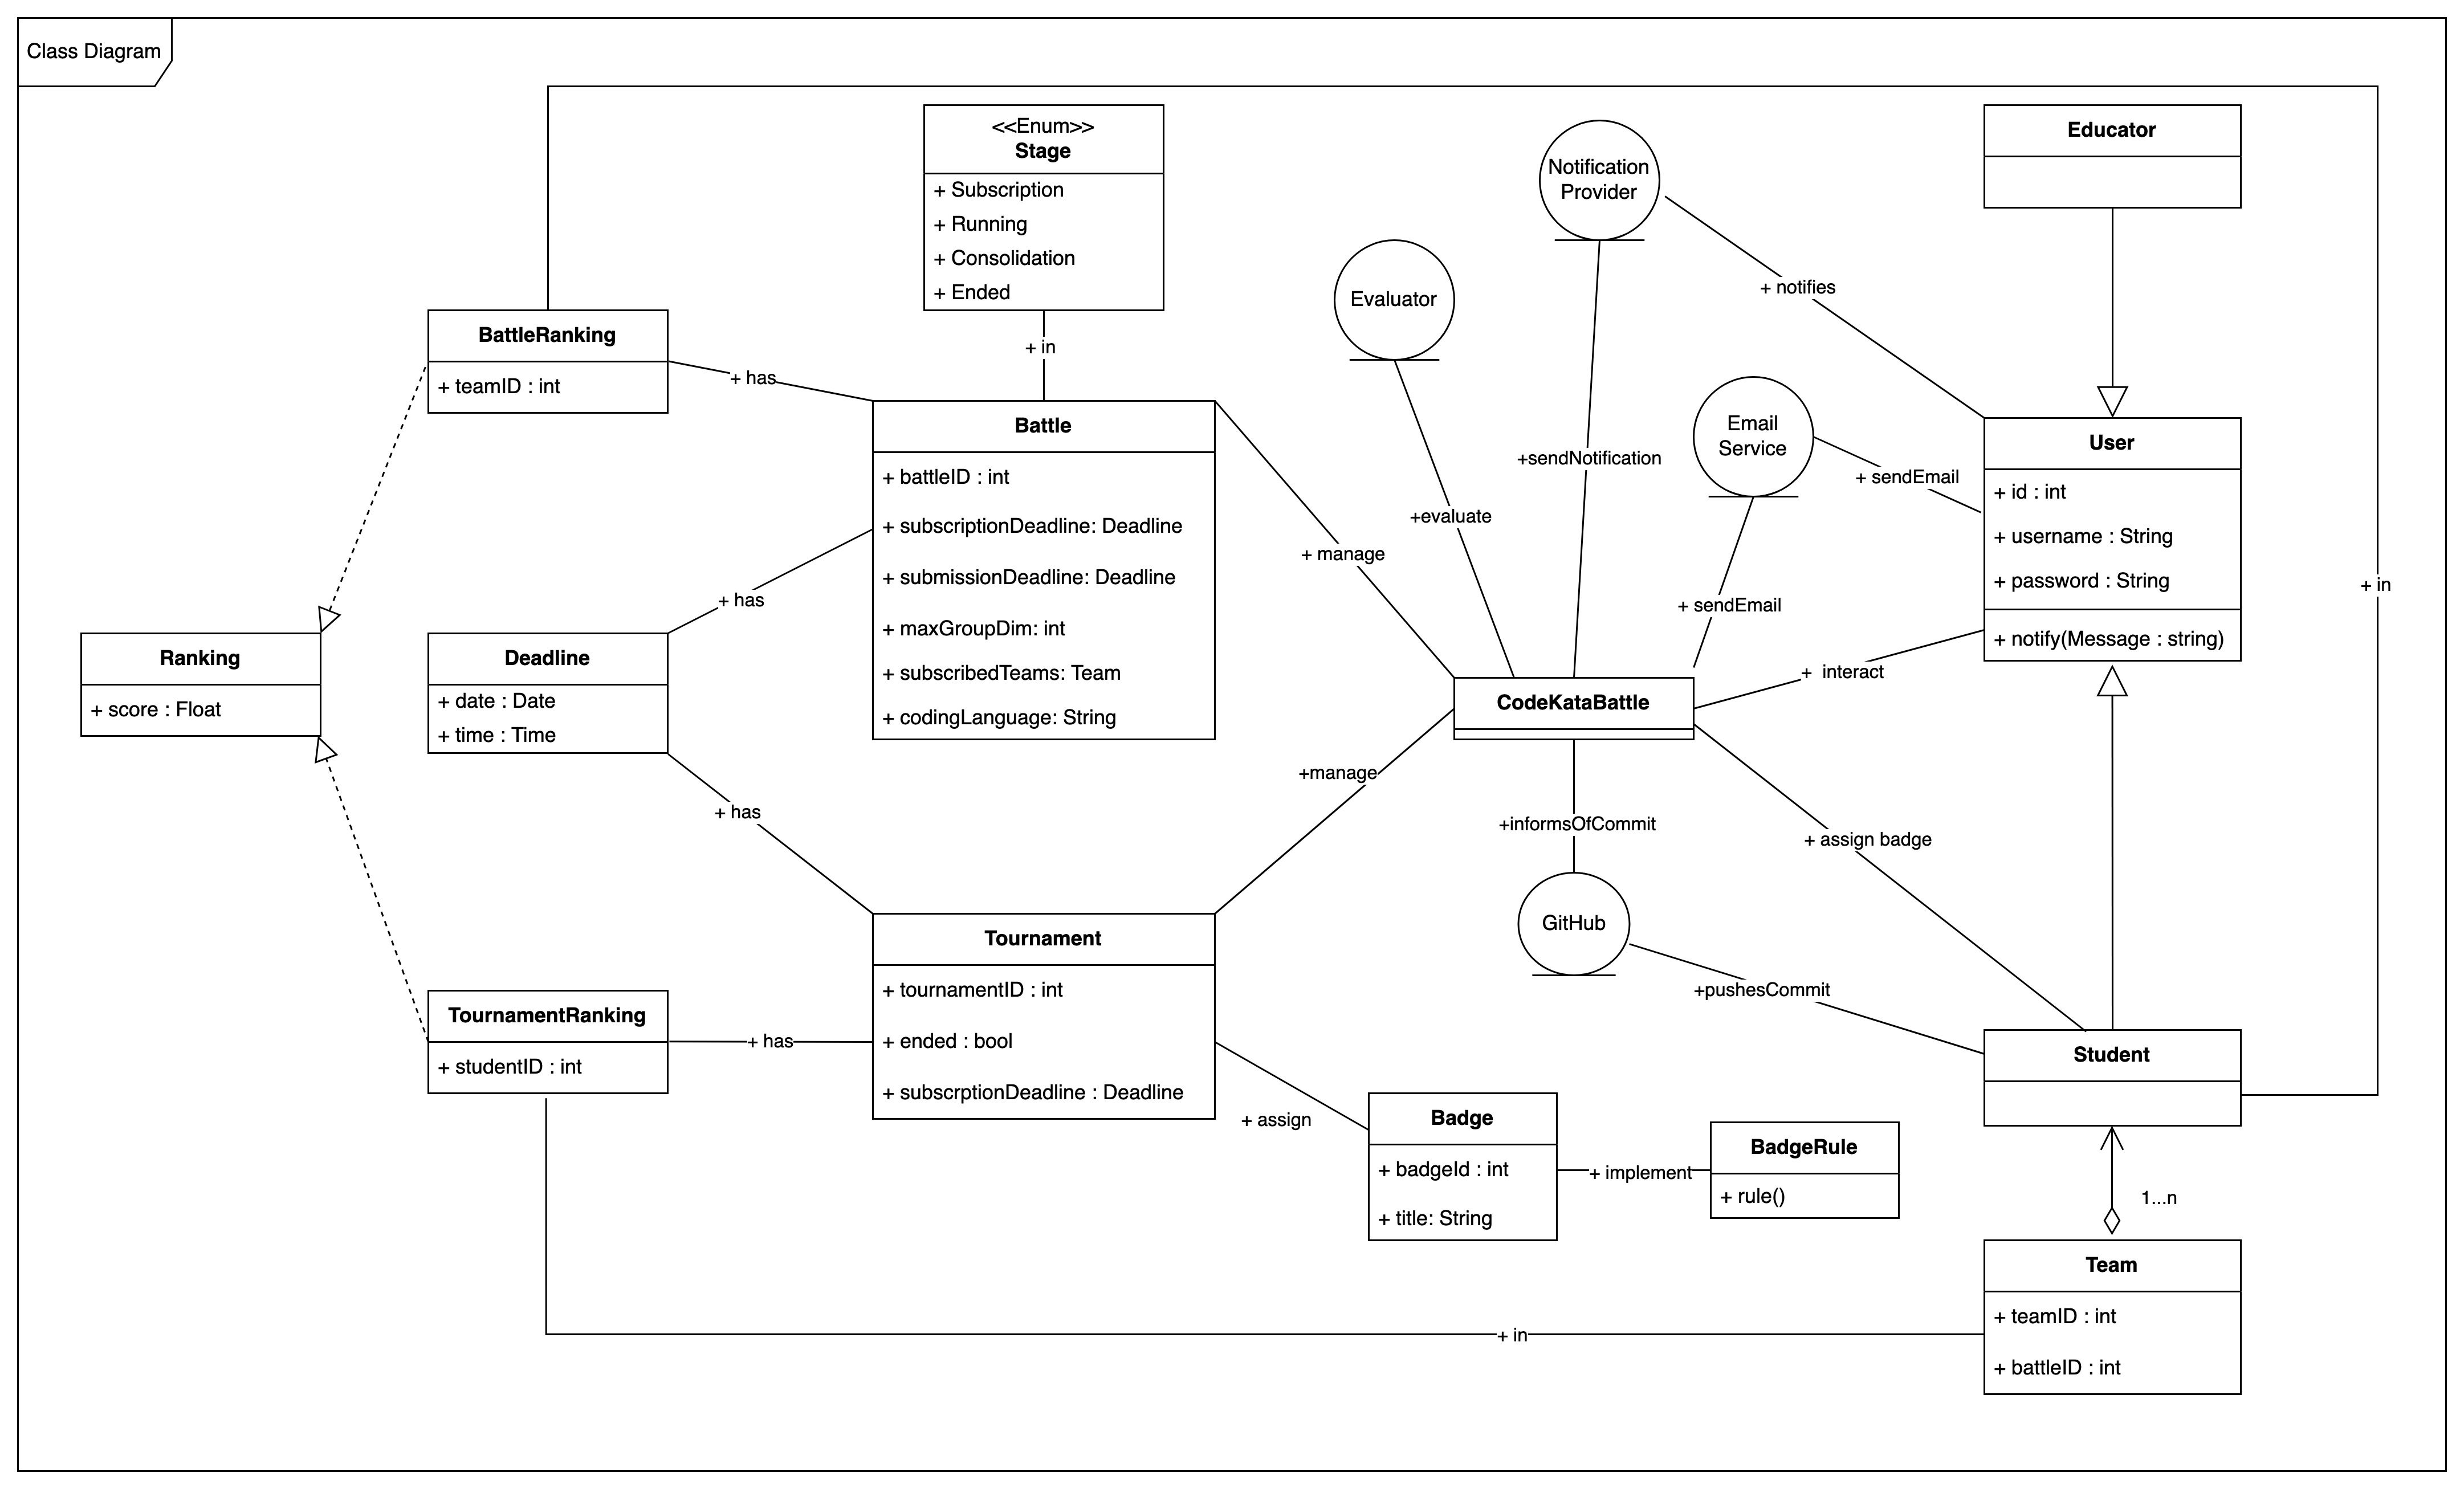
\includegraphics[scale = 0.45]{Images/ClassDiagram/ClassDiagram.png}\\
\centering
\end{figure}

{\color{bluepoli}\rule{\linewidth}{0.1pt}}

\subsection{State Charts}

{\color{bluepoli}\rule{\linewidth}{0.1pt}}

The subsequent section details the principal elements of the CodeKataBattle (CKB) system and their progression through different phases. For this purpose, some UML State Charts are proposed.

\begin{figure}[H]
\textbf{Tournament}\par\medskip
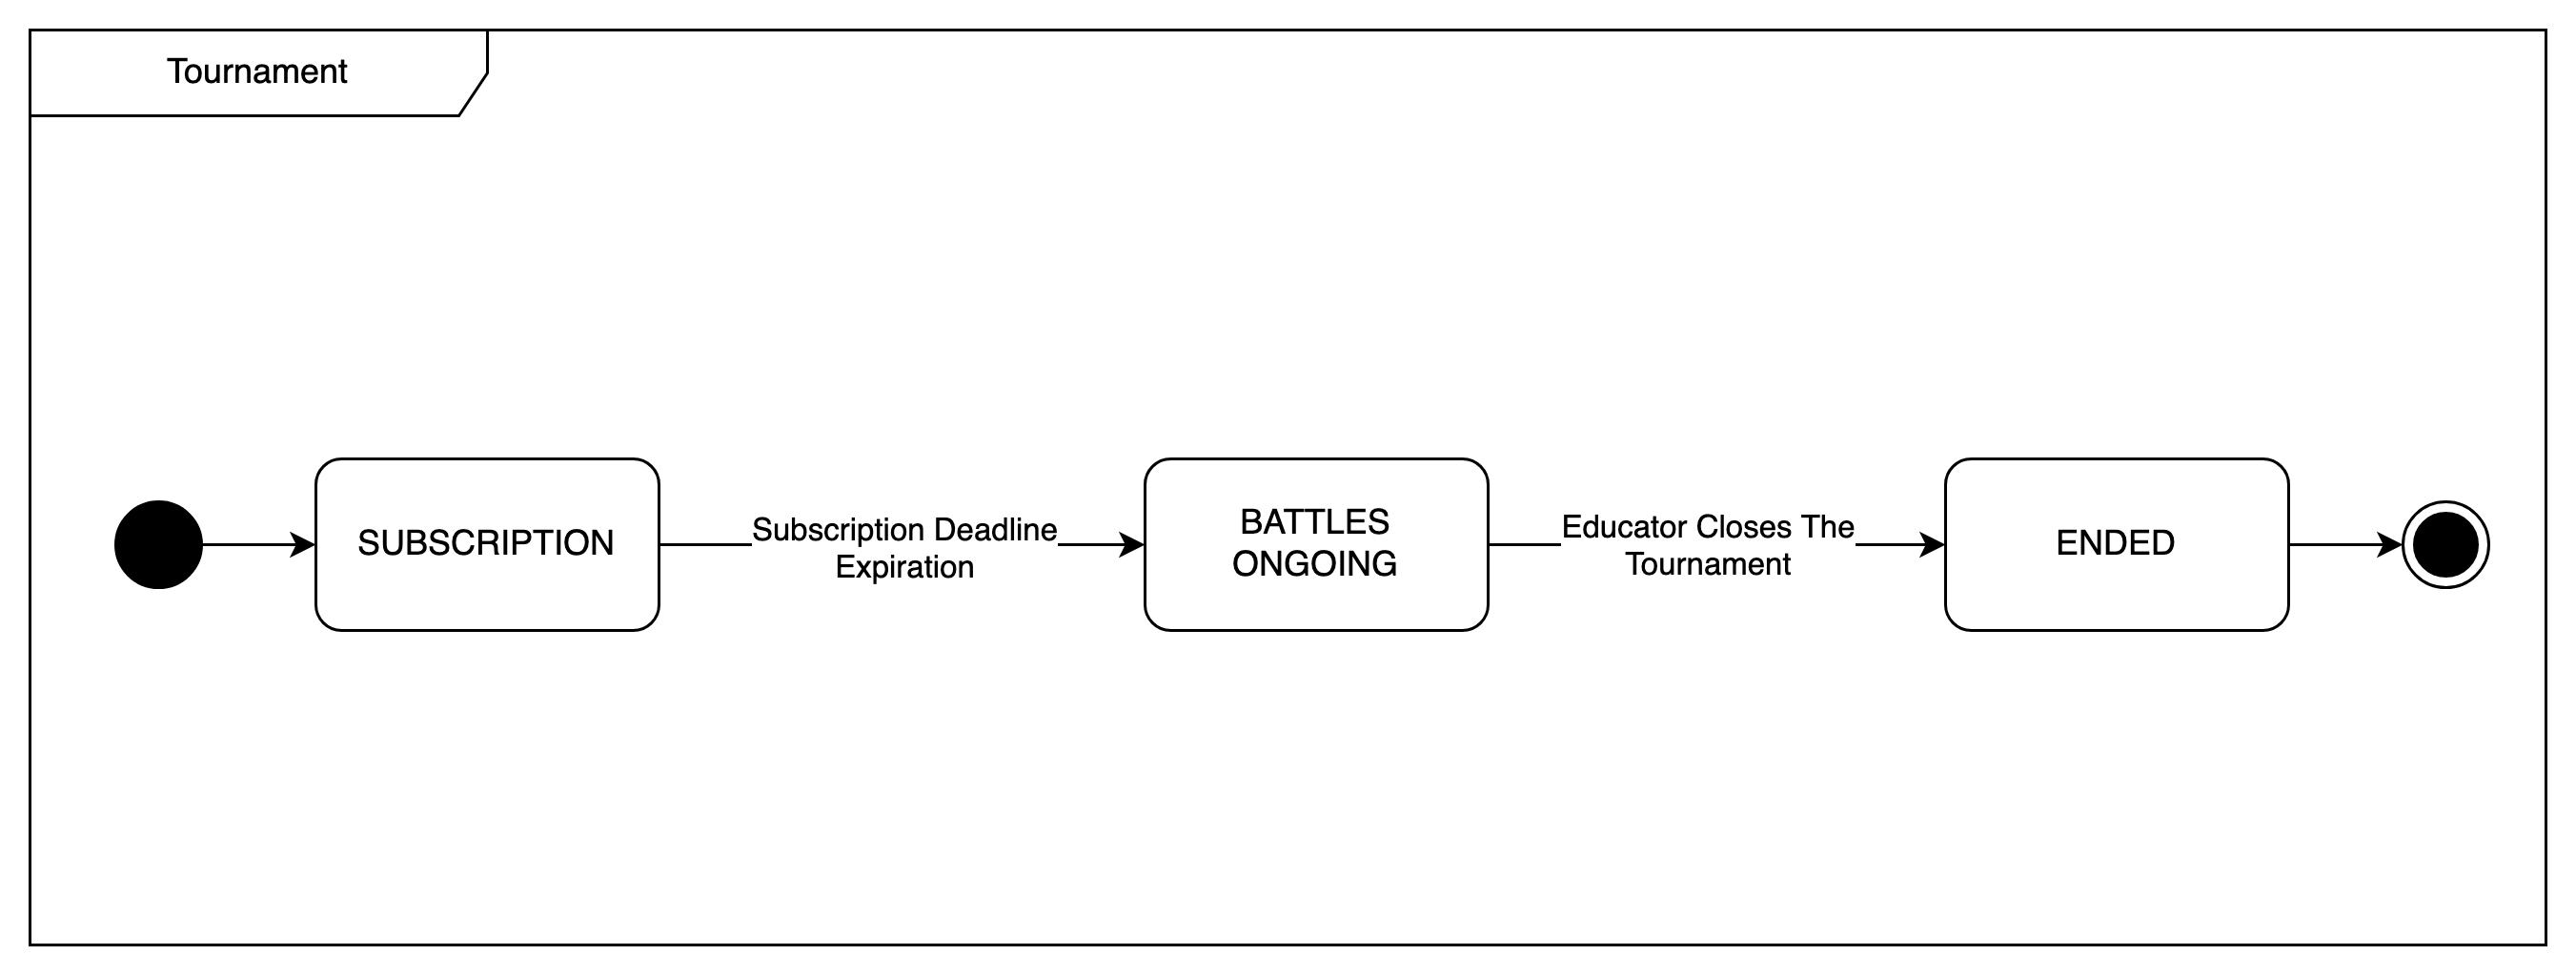
\includegraphics[scale = 0.45]{Images/StateCharts/TournamentStateDiagram.png}\\
\centering
\end{figure}

\begin{itemize}
\item The diagram in question outlines the potential phases of a Tournament. Initiated by an Educator, the Tournament promptly enters the 'Subscription' phase, allowing Students to register their participation. Following the closure of the subscription window, the system transitions the Tournament to the 'Ongoing' phase, wherein Battles are created and unfold. Upon the resolution of these contests, the Educator finalizes the Tournament, propelling it into the 'Ended' phase.
\end{itemize}

\begin{figure}[H]
\textbf{Tournament}\par\medskip
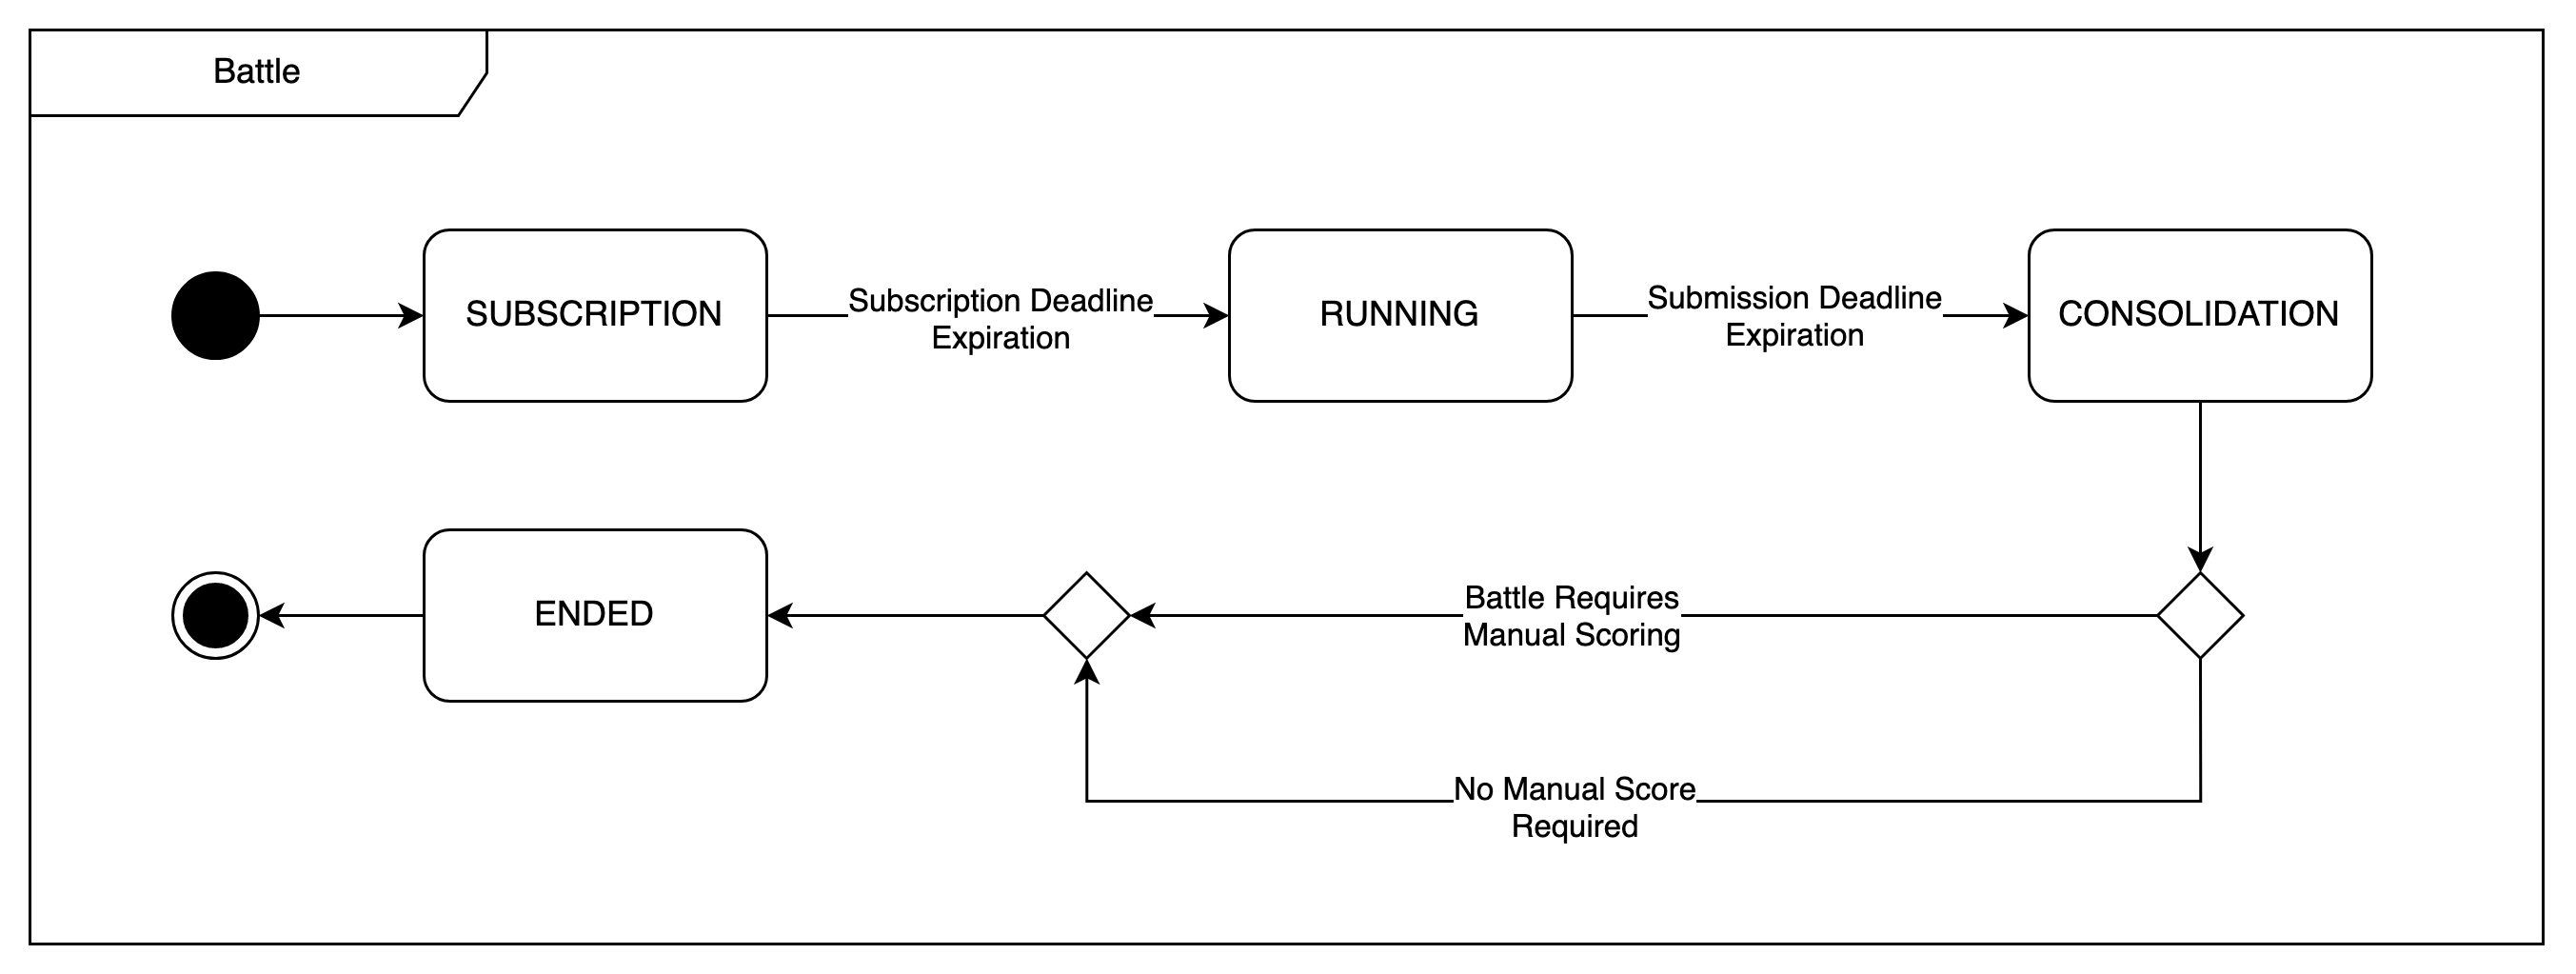
\includegraphics[scale = 0.45]{Images/StateCharts/BattleStateDiagram.png}\\
\centering
\end{figure}

\begin{itemize}
\item The second state diagram offers an overview of the stages a Battle undergoes on the CKB platform. Once the Educator creates a Battle, it is set in "SUBSCRIPTION" state, where Students can form teams and register for the challenge. Following the end of the subscription deadline, the Battle transitions to the "RUNNING" state. This phase is characterized by active participation as Students develop solutions and submit their code before the submission deadline. After the submission deadline has passed, the platform moves the Battle into the "CONSOLIDATION" phase, which is a critical juncture where the platform assesses the submissions. Depending on the Battle's configuration, there may be a need for manual scoring by Educators. If so, the Educators review the submissions and assign additional scores. Once the manual evaluation is complete, or if no manual scoring is necessary, the Battle proceeds to the "ENDED" state, signaling its conclusion and the finalization of results and rankings.
\end{itemize}

{\color{bluepoli}\rule{\linewidth}{0.1pt}}

\section{Product Functions}

The platform CKB offers several key functions:

\begin{itemize}
\item \textcolor{bluepoli}{Battles and Tournaments Creation} Educators can create coding challenges (Battles) within Tournaments, specifying details like descriptions, team sizes, deadlines, scoring configurations and, eventually, Badges.
\item \textcolor{bluepoli}{Student Participation} On the other hand, Students can join such Tournaments and take part in Battles, individually or in teams. 
\item \textcolor{bluepoli}{GitHub Integration} The system allows the Students to perform code submissions just by pushing their code on GitHub, thanks to automated workflows triggered by GitHub Actions service.
\item \textcolor{bluepoli}{Automated Evaluation} The platform automatically evaluates Student code based on test cases, timeliness, and code quality using external static analysis tools.
\item \textcolor{bluepoli}{Scoring and Ranking} It continuously updates team rankings during Battles and provides overall Tournament rankings at the end of each Battle.
\item \textcolor{bluepoli}{Badges and Recognition} Educators define Badges which can be obtained by Students, serving as recognition for accomplishments and participation to a certain Tournament.
\item \textcolor{bluepoli}{Manual Optional Evaluation} Educators can manually evaluate Students' work and assign additional scores at the end of every Battle.
\end{itemize}

{\color{bluepoli}\rule{\linewidth}{0.1pt}}

\subsection{Requirements}

{\color{bluepoli}\rule{\linewidth}{0.1pt}}

\begin{enumerate}
    \item[\textcolor{bluepoli}{R1}] The system must allow an unregistered Educator to sign up.
    \item[\textcolor{bluepoli}{R2}] The system must allow an unregistered Student to sign up.
    \item[\textcolor{bluepoli}{R3}] The system must allow a registered User to log in.
    \item[\textcolor{bluepoli}{R4}] The system must allow registered Educators to start the creation process of a Tournament of Code Kata Battles.
    \item[\textcolor{bluepoli}{R5}] The system must provide registered Educators of a list of Tournament-related statistics for the Badges definition, during the Tournament creation process.
    \item[\textcolor{bluepoli}{R6}] The system must provide registered Educators of a specific language which lets them define the Badges, during the Tournament creation process.
    \item[\textcolor{bluepoli}{R7}] The system must allow registered Educators to grant other registered Educators the permission to manage the Tournament, during the Tournament creation process.
    \item[\textcolor{bluepoli}{R8}] The system must allow registered Educators to end the creation process of a Tournament that they started themselves.
    \item[\textcolor{bluepoli}{R9}] The system must be able to send notifications to every registered User.
    \item[\textcolor{bluepoli}{R10}] The system must allow a registered Educator to create a Battle in a Tournament if and only if he is the creator of the Tournament or if he was granted the permission to by the latter.
    \item[\textcolor{bluepoli}{R11}] The system must allow a registered Student to create a group for a Battle in a Tournament.
    \item[\textcolor{bluepoli}{R12}] The system must allow a registered Student to accept an invitation to a group for a Battle in a Tournament.
    \item[\textcolor{bluepoli}{R13}] The system must allow registered Students to see the list of ongoing Tournaments and join any of those if its subscription deadline is not expired yet.
    \item[\textcolor{bluepoli}{R14}] The system must allow registered Students who are enrolled in a Battle to perform code submissions.
    \item[\textcolor{bluepoli}{R15}] The system must be provided of proper APIs to let registered Students perform code submissions through GitHub Actions.
    \item[\textcolor{bluepoli}{R16}] The system must update the Battle ranking when a valid code submission is performed.
    \item[\textcolor{bluepoli}{R17}] The system must set the Consolidation Stage of a Battle when its submission deadline expires.
    \item[\textcolor{bluepoli}{R18}] The system must let Educators to end the Consolidation Stage of a Battle if and only if he is the creator of the Tournament or if he was granted the permission to by the latter.
    \item[\textcolor{bluepoli}{R19}] The system must update Tournament ranking when a Battle exits the Consolidation Stage.
    \item[\textcolor{bluepoli}{R20}] The system must let Educators who are either the creator of the Tournament or who have been granted the permission to by the latter to close a Tournament if and only if there is no Battle such that either their subscription or submission deadline is not expired yet or such that they are still in the Consolidation Stage.
    \item[\textcolor{bluepoli}{R21}] The system must assign an achievements’ Badge for a given Tournament to any Student who satisfied the conditions defined by the creator of the Tournament.
    \item[\textcolor{bluepoli}{R22}] The system must allow every User to see the Badges which were ever obtained by a given Student.
    \item[\textcolor{bluepoli}{R23}] The system must notify every registered Student about the creation of a new Tournament.
    \item[\textcolor{bluepoli}{R24}] The system must notify every registered Student about the creation of a new Battle within a Tournament they are enrolled in.
    \item[\textcolor{bluepoli}{R25}] The system must notify every registered Student about the end of a Battle they are participating in.
    \item[\textcolor{bluepoli}{R26}] The system must notify every registered Student about the end of a Tournament they are enrolled in.
\end{enumerate}

{\color{bluepoli}\rule{\linewidth}{0.1pt}}

\section{User Characteristics}

In the CKB platform, a User can be either a Student or an Educator, each with distinct roles and motivations.

\begin{itemize}
\item \textcolor{bluepoli}{Students} They join Battles to practice coding in a collaborative environment, aiming to enhance their programming skills through practical challenges, seeking to measure their performance against peers and track their progress. Students can achieve recognition by obtaining Badges within the context of a Tournament. Students are often notified about new activities that they may want to join, such as a new Tournament, or a new Battle within the context of a Tournament that they are enrolled in.
\item \textcolor{bluepoli}{Educators} They set up and manage the coding challenges, individually or cooperating with other Educators. They act as facilitators, creating Battles within Tournaments to engage Students in practical exercises. Educators may want to personally evaluate Students' code submissions, in order to reward particularly brilliant solutions or to penalize major mistakes. Additionally, they are responsible for defining Badge criteria, which act as a motivating factor.
\end{itemize}

{\color{bluepoli}\rule{\linewidth}{0.1pt}}

\section{Assumptions, Dependencies, Constraints}

This section serves as a comprehensive overview of critical factors which must be considered during the implementation of the platform. It consolidates the foundational assumptions made during project planning and highlights eventual dependencies.

{\color{bluepoli}\rule{\linewidth}{0.1pt}}

\subsection{Domain Assumptions}

{\color{bluepoli}\rule{\linewidth}{0.1pt}}t

\begin{enumerate}
    \item[\textcolor{bluepoli}{D1}] The User must have a working Internet connection.
    \item[\textcolor{bluepoli}{D2}] The Students who participate to a Battle properly set up the GitHub Action for code submissions.
    \item[\textcolor{bluepoli}{D3}] The Users always receive every notification which is sent by the system.
    \item[\textcolor{bluepoli}{D4}] The availability of the static analysis tools utilized for the code evaluation process is consistent.
    \item[\textcolor{bluepoli}{D5}] The availability of GitHub Actions service is consistent.
\end{enumerate}

{\color{bluepoli}\rule{\linewidth}{0.1pt}}

\subsection{Dependencies}

{\color{bluepoli}\rule{\linewidth}{0.1pt}}

The static analysis tools which provide a score based on the quality level of each code submission can either be implemented or integrated in the system as Evaluator. Similarly, the NotificationProvider can either be implemented or integrated in the system. For the registration process, a verification email must be sent by the system through to let Users successfully sign up, thus requiring the integration of an EmailService.

{\color{bluepoli}\rule{\linewidth}{0.1pt}}


% THIRD CHAPTER
% --------------------------------------------------------------------------
\chapter{Specific requirements}

\section{External Interface Requirements}

The system provides all the main functions described previously (see section 2.2) and lets Users access all the information they are granted permission for. Given such purposes, any personal computer is a suitable device to make use of all the CKB functionalities, allowing convenient acces through any web browser.

\subsection{User Interfaces}

{\color{bluepoli}\rule{\linewidth}{0.1pt}}

\begin{figure}[H]
\centering
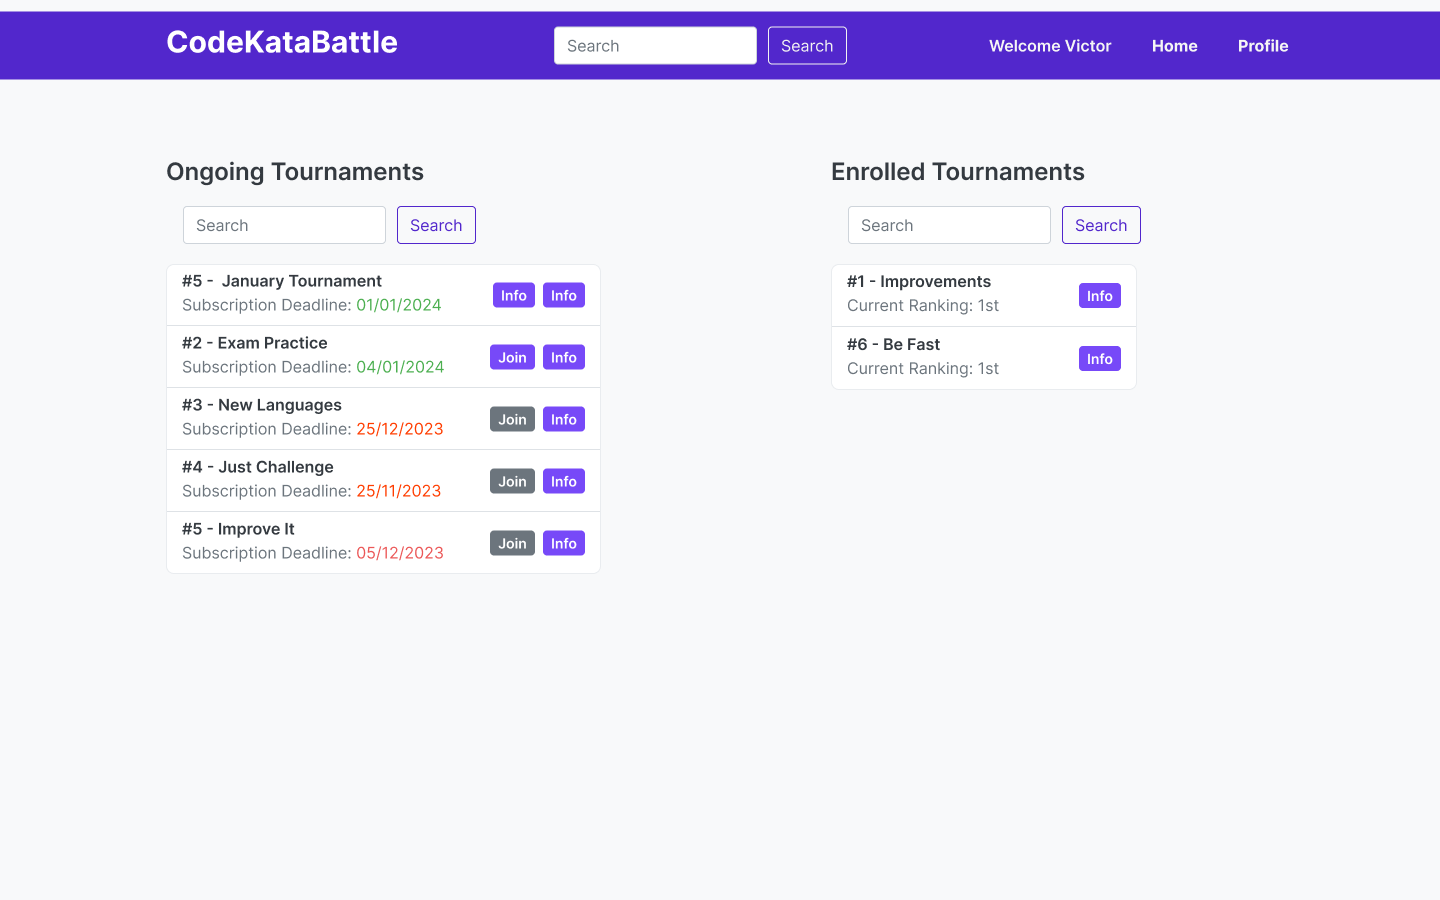
\includegraphics[scale = 0.25]{Images/UI/MainPage_Student.png}\\
\caption{Home Page (Student)}
\end{figure}

\begin{figure}[H]
\centering
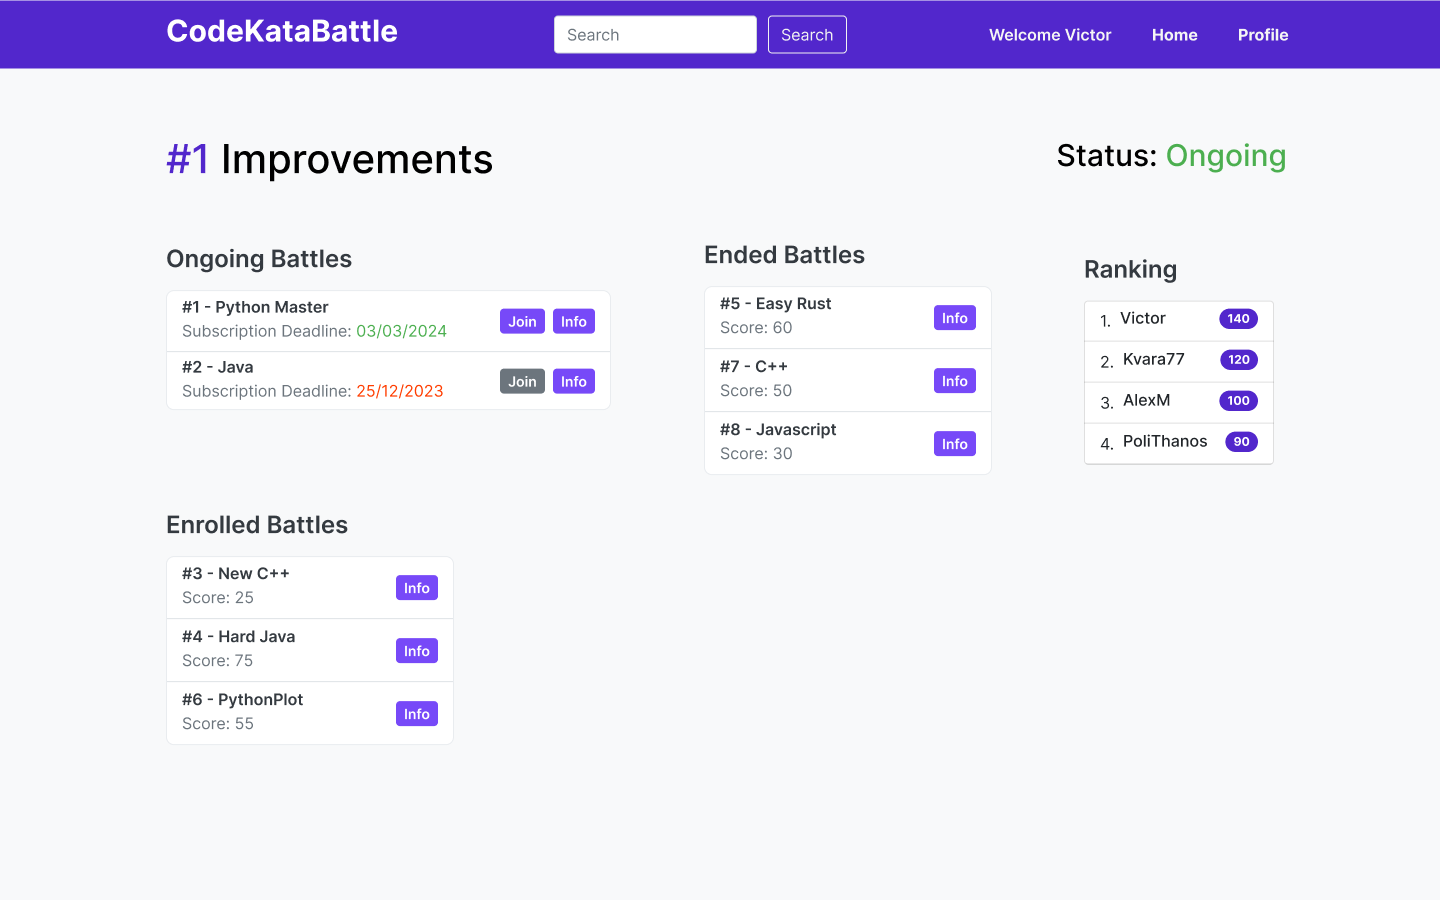
\includegraphics[scale = 0.25]{Images/UI/TournamentPage_Student.png}\\
\caption{Tournament Page (Student)}
\end{figure}

\begin{figure}[H]
\centering
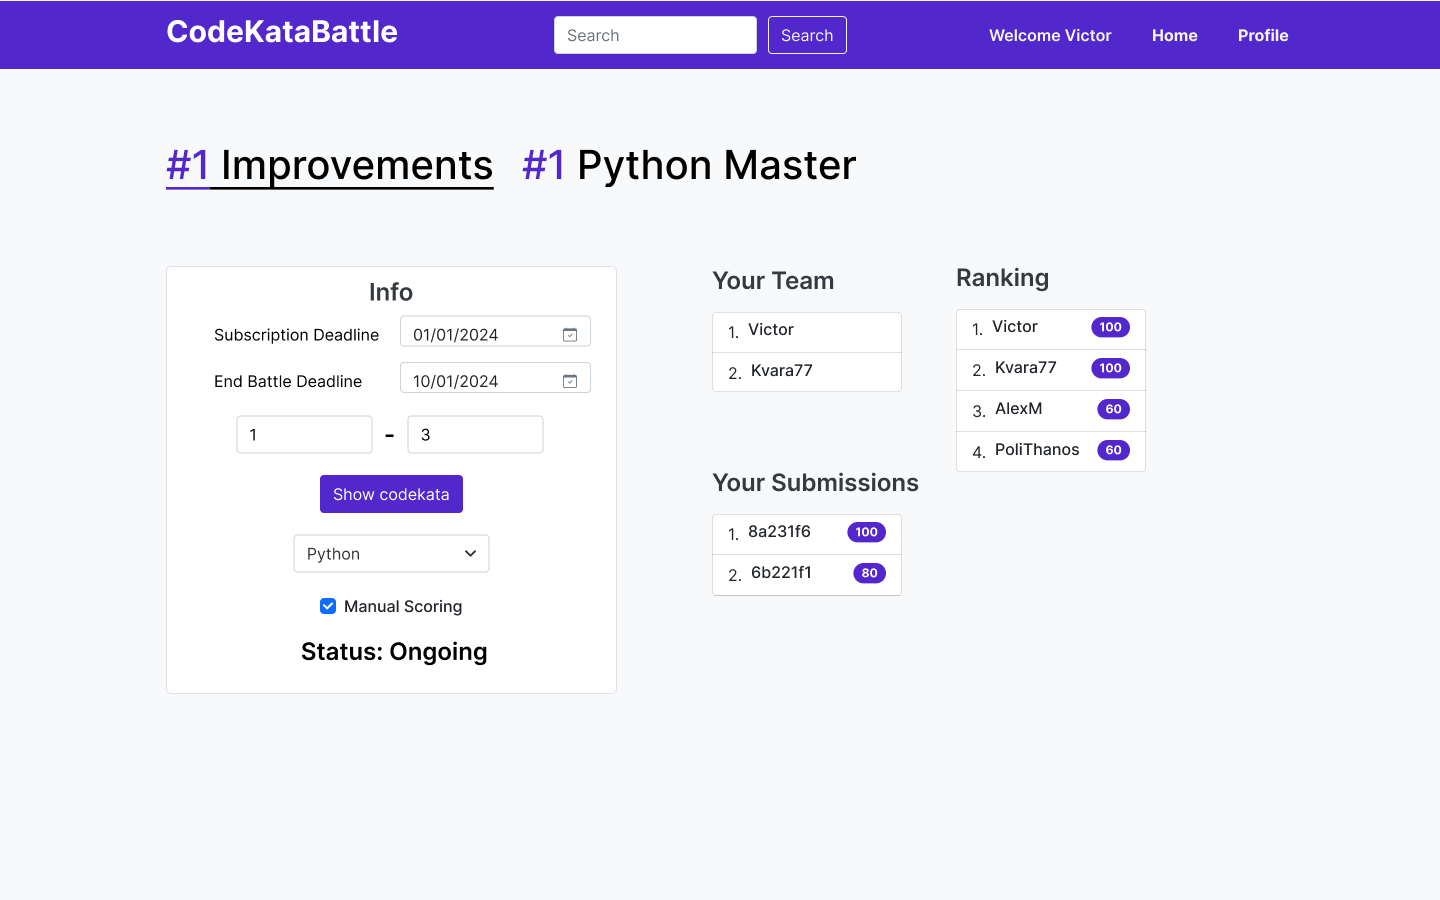
\includegraphics[scale = 0.25]{Images/UI/BattlePage_Student.png}\\
\caption{Battle Page (Student)}
\end{figure}

\begin{figure}[H]
\centering
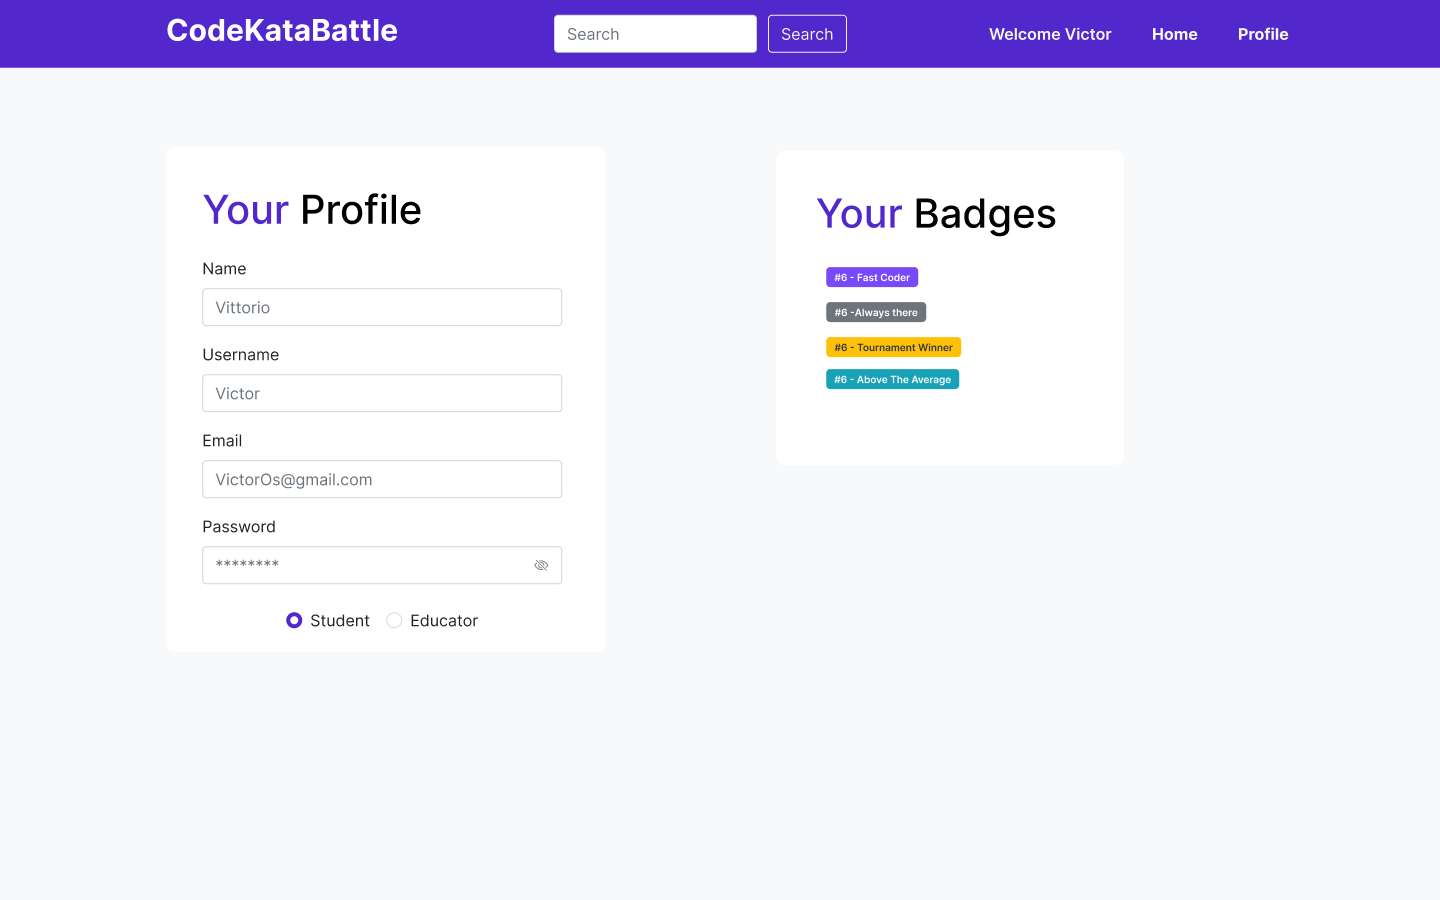
\includegraphics[scale = 0.25]{Images/UI/Profile_Student.png}\\
\caption{Profile Page (Student) }
\end{figure}

\begin{figure}[H]
\centering
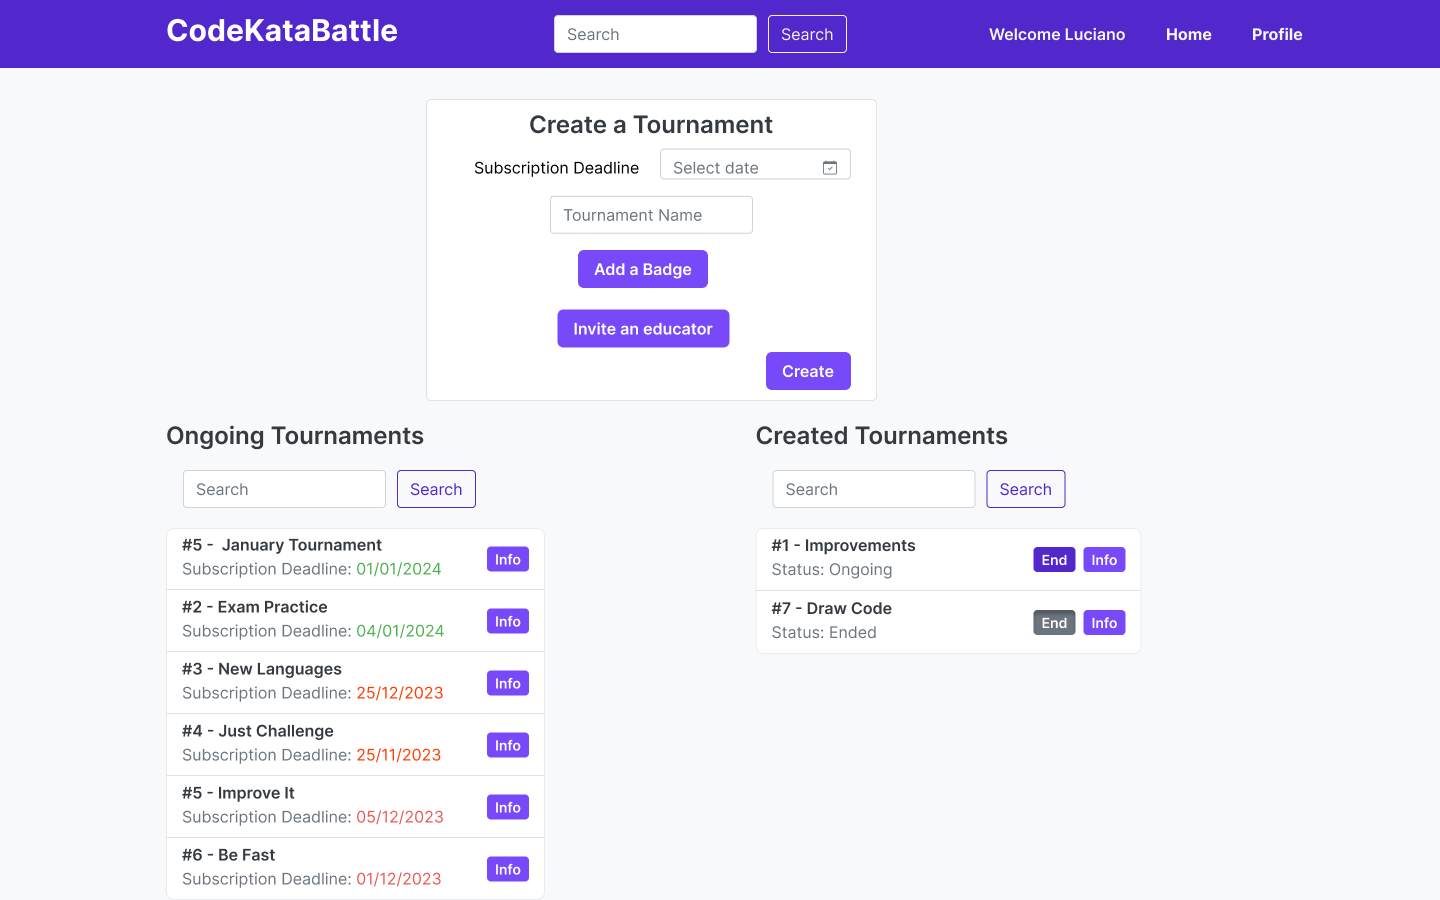
\includegraphics[scale = 0.25]{Images/UI/MainPageEducator.png}\\
\caption{Home Page (Educator)}
\end{figure}

\begin{figure}[H]
\centering
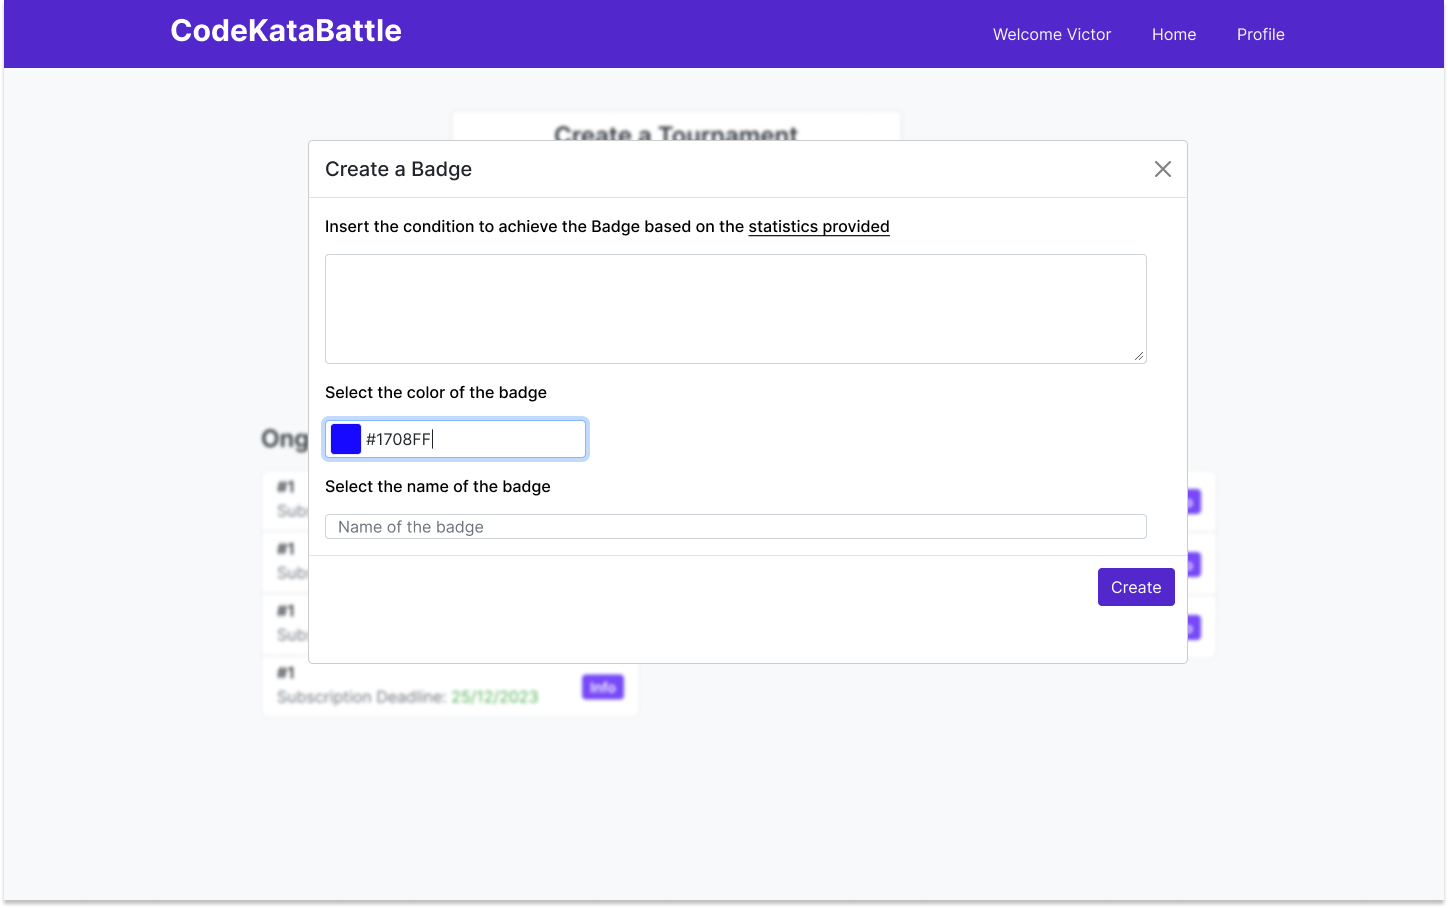
\includegraphics[scale = 0.25]{Images/UI/MainPageEducator-1.png}\\
\caption{Badge definition for a tournament (Educator)}
\end{figure}

\begin{figure}[H]
\centering
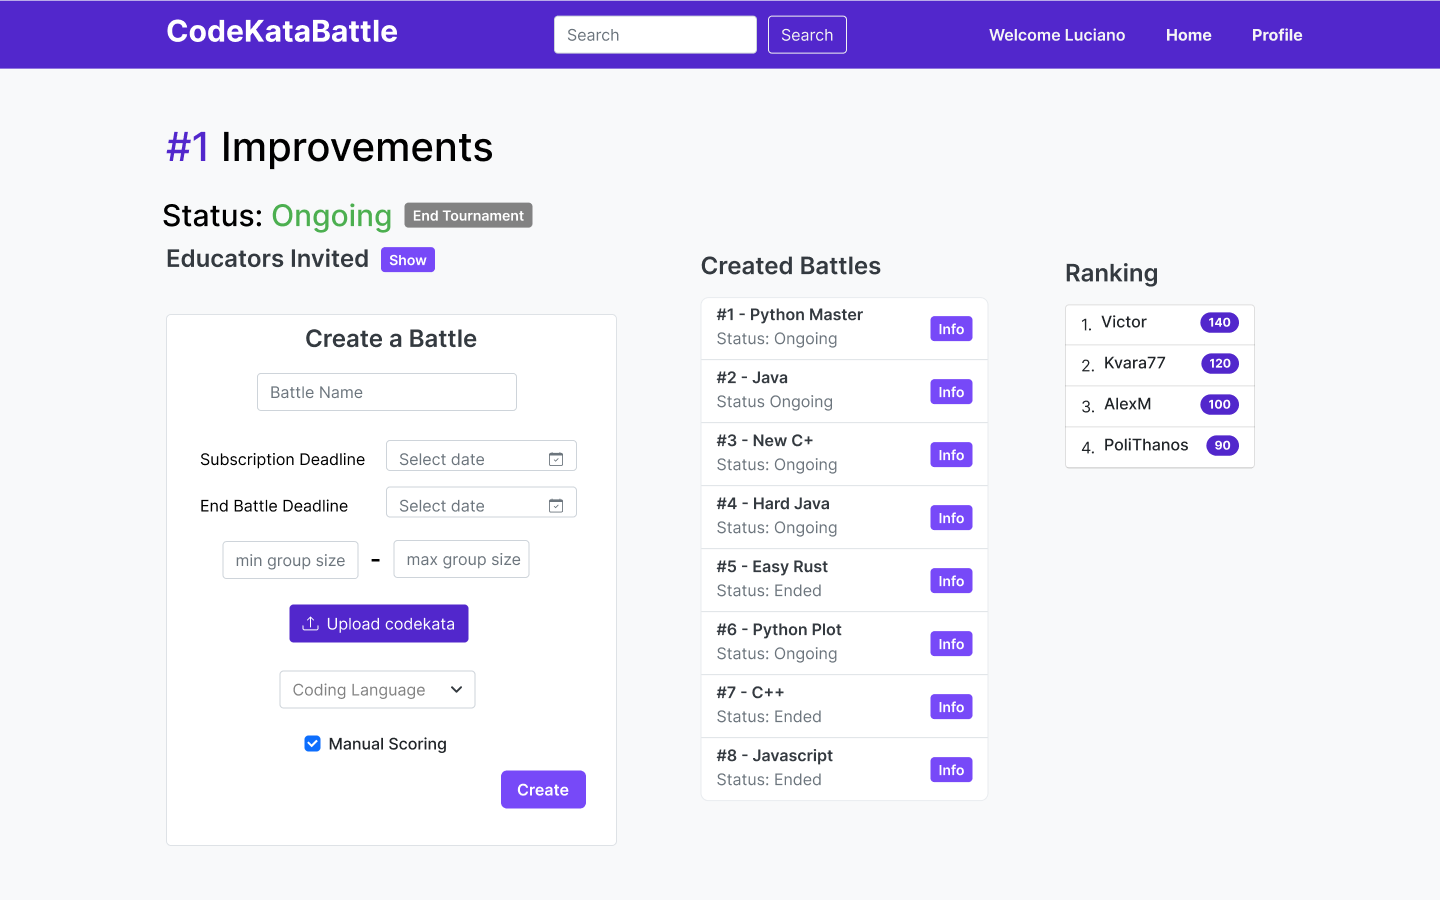
\includegraphics[scale = 0.25]{Images/UI/TournamentPage_EducatorCreator.png}\\
\caption{Tournament Page where the educator is the creator of the tournament (Educator)}
\end{figure}

\begin{figure}[H]
\centering
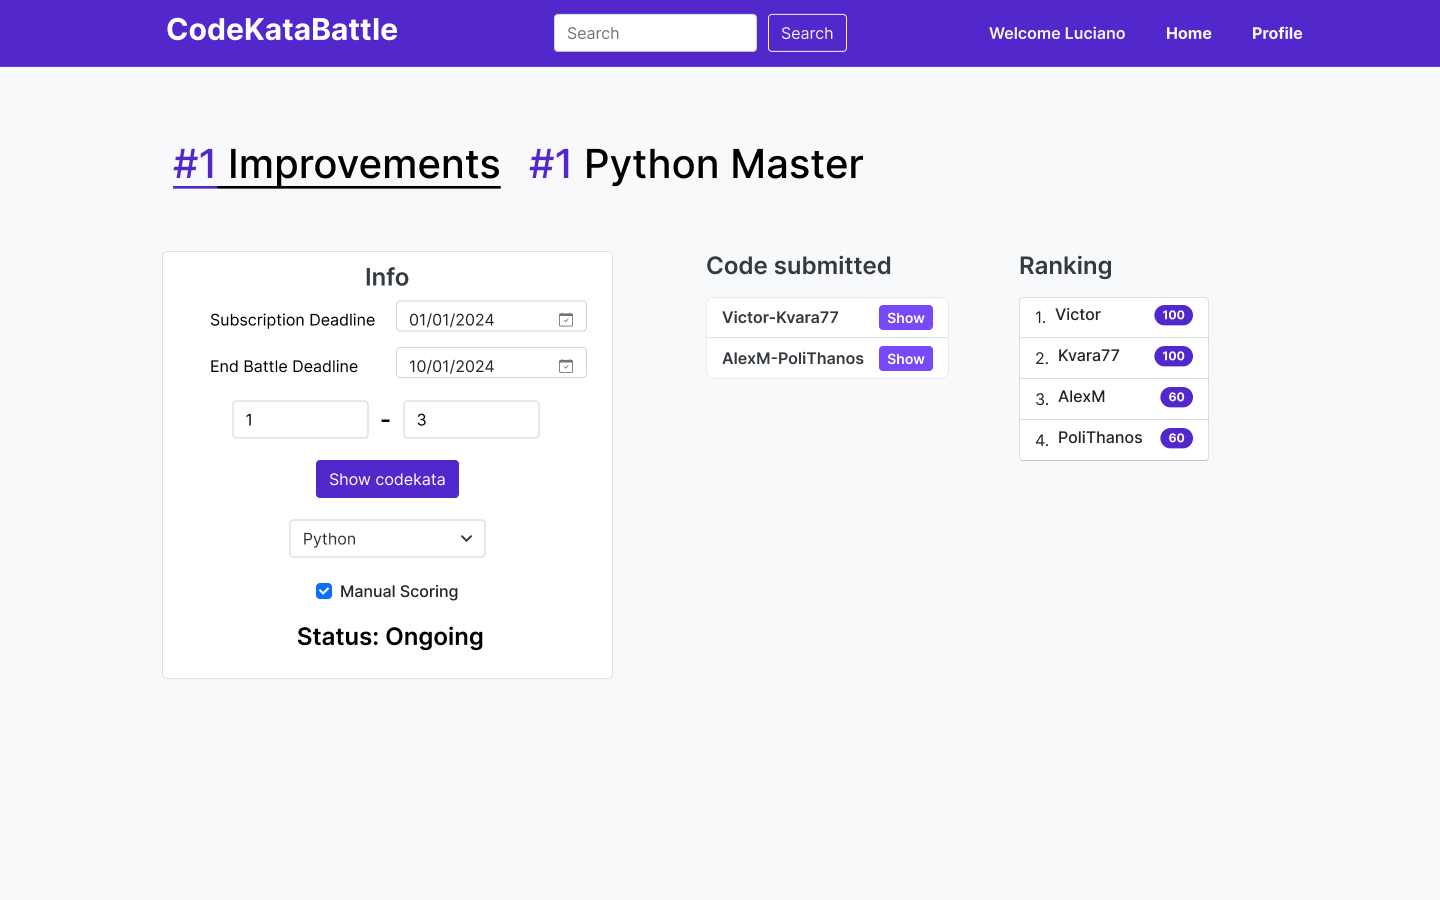
\includegraphics[scale = 0.25]{Images/UI/BattlePage_EducatorCreator.png}\\
\caption{Battle Page where the educator is the creator of the tournament (Educator)}
\end{figure}








{\color{bluepoli}\rule{\linewidth}{0.1pt}}

\subsection{Hardware Interfaces}

{\color{bluepoli}\rule{\linewidth}{0.1pt}}

To use the system, both Educators and Students must use a suitable device. Due to the communication capabilities needed, any personal computer results once again being a suitable device for the User purpose. \\

{\color{bluepoli}\rule{\linewidth}{0.1pt}}

\subsection{Software Interfaces}

{\color{bluepoli}\rule{\linewidth}{0.1pt}}

The system should integrate a NotificationService to keep up Users of any interesting event on the platform, an EmailService for the registration process, and proper static analysis tools as an Evaluator of the Students' code submissions.\\

{\color{bluepoli}\rule{\linewidth}{0.1pt}}

\subsection{Communication Interfaces}

{\color{bluepoli}\rule{\linewidth}{0.1pt}}

The system requires a stable internet connection to work properly. This connection is used to exchange data between the Users and the central database which contains the information regarding ongoing Tournaments and Battles.\\

{\color{bluepoli}\rule{\linewidth}{0.1pt}}

\section{Functional Requirements}

In this section, all the Use Cases are listed attached to their corresponding Use Case Diagram. Then, the mapping between Goals, Domain Assumptions and Requirements is provided.\\
{\color{bluepoli}\rule{\linewidth}{0.1pt}}

\subsection{Use Case Diagrams}

{\color{bluepoli}\rule{\linewidth}{0.1pt}}

\begin{figure}[H]
    \centering
    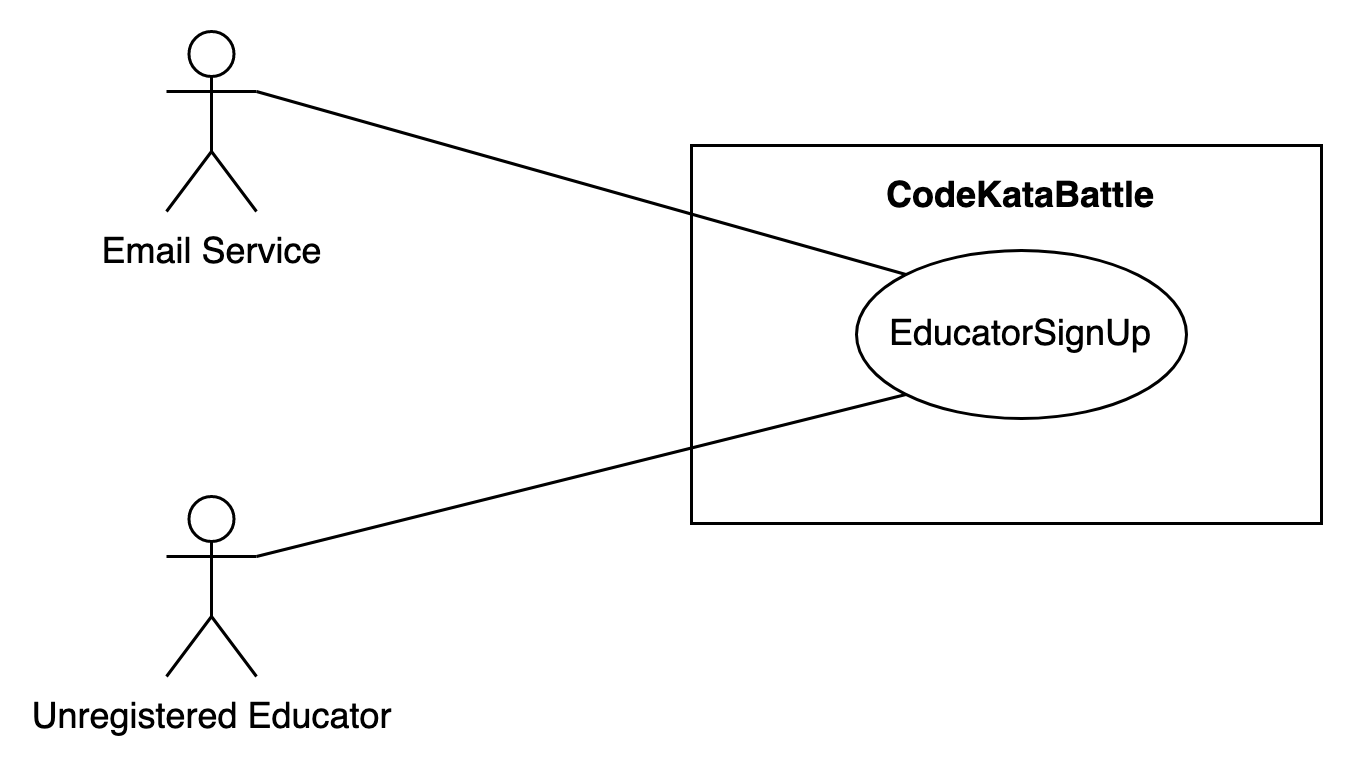
\includegraphics[scale = 0.45]{Images/UseCaseDiagrams/EducatorSignUpUseCaseDiagram.png}\\
    \caption{EducatorSignUp}
    \centering
\end{figure}
\begin{figure}[H]
    \centering
    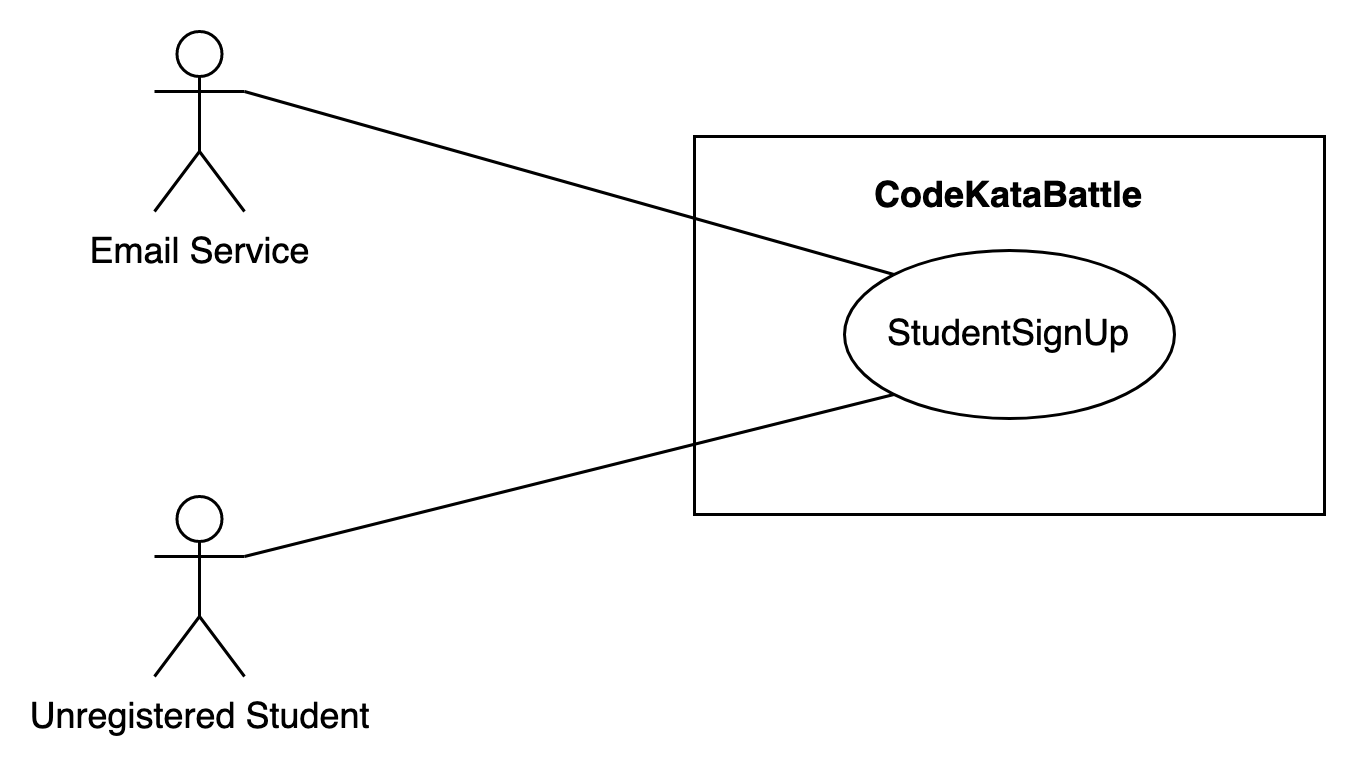
\includegraphics[scale = 0.45]{Images/UseCaseDiagrams/StudentSignUpUseCaseDiagram.png}\\
    \caption{StudentSignUp}
\end{figure}
\begin{figure}[H]
    \centering
    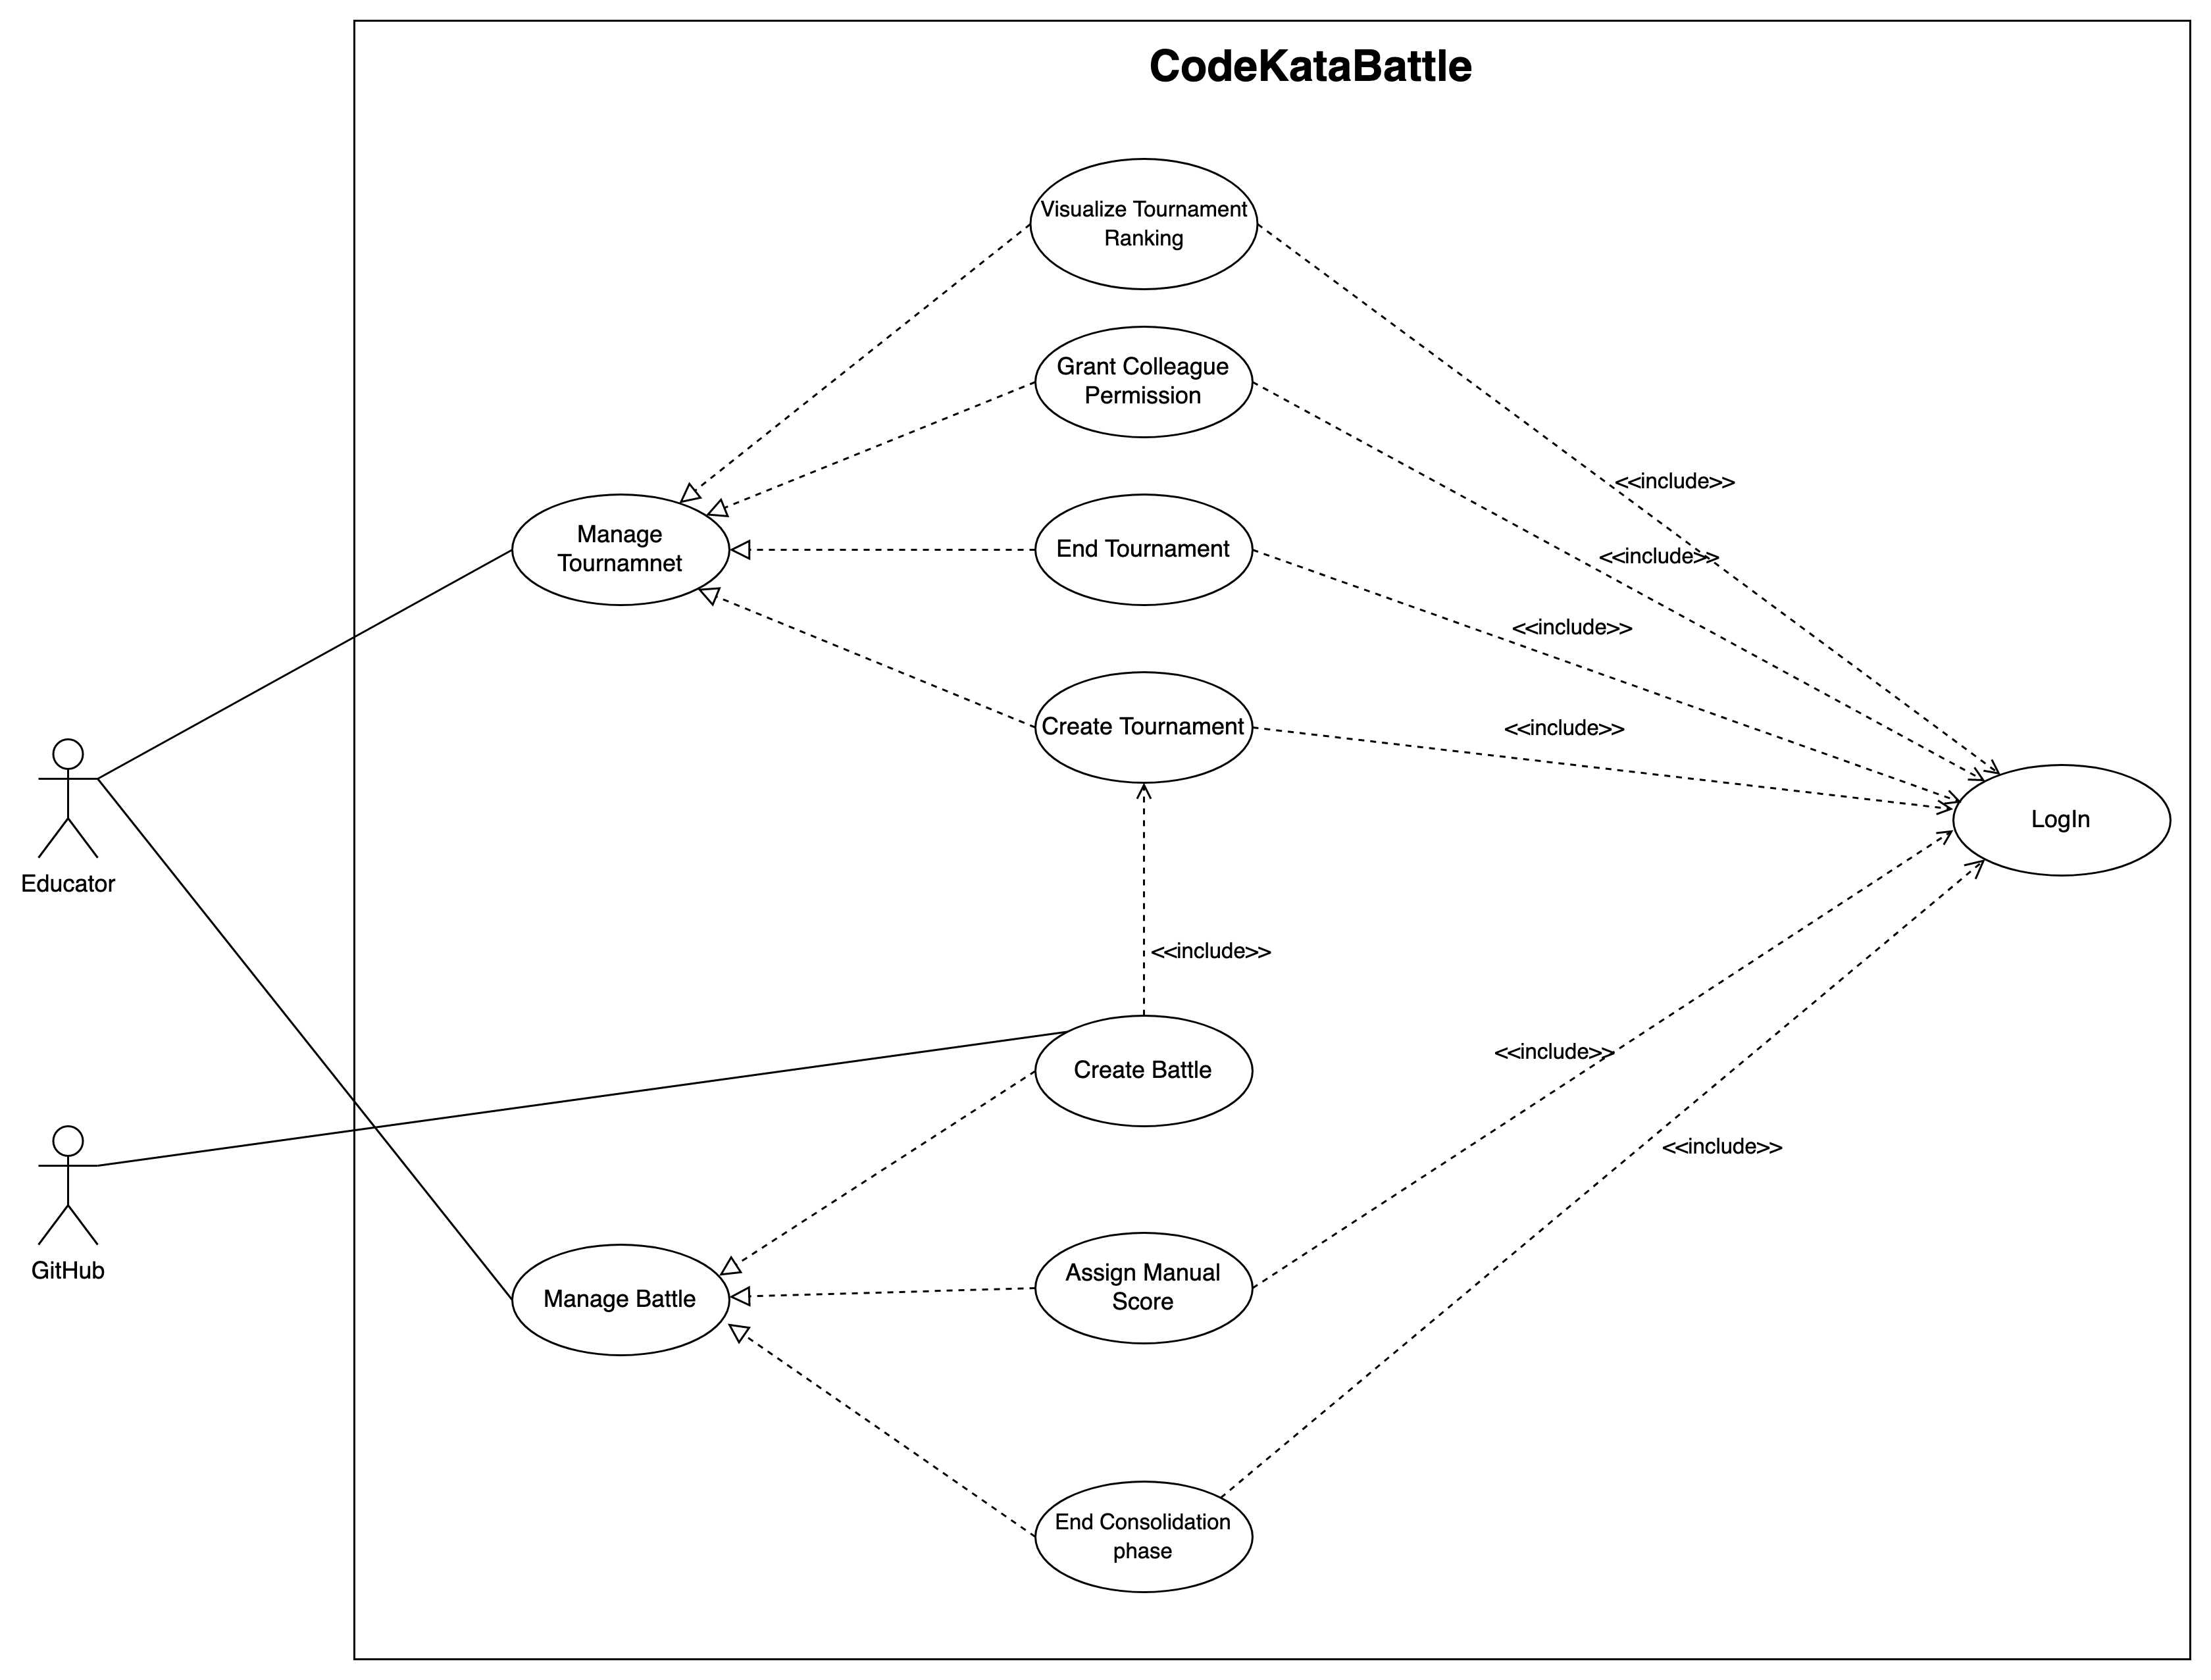
\includegraphics[scale = 0.45]{Images/UseCaseDiagrams/EducatorUseCaseDiagram.png}\\
    \caption{Educator}
\end{figure}
\begin{figure}[H]
    \centering
    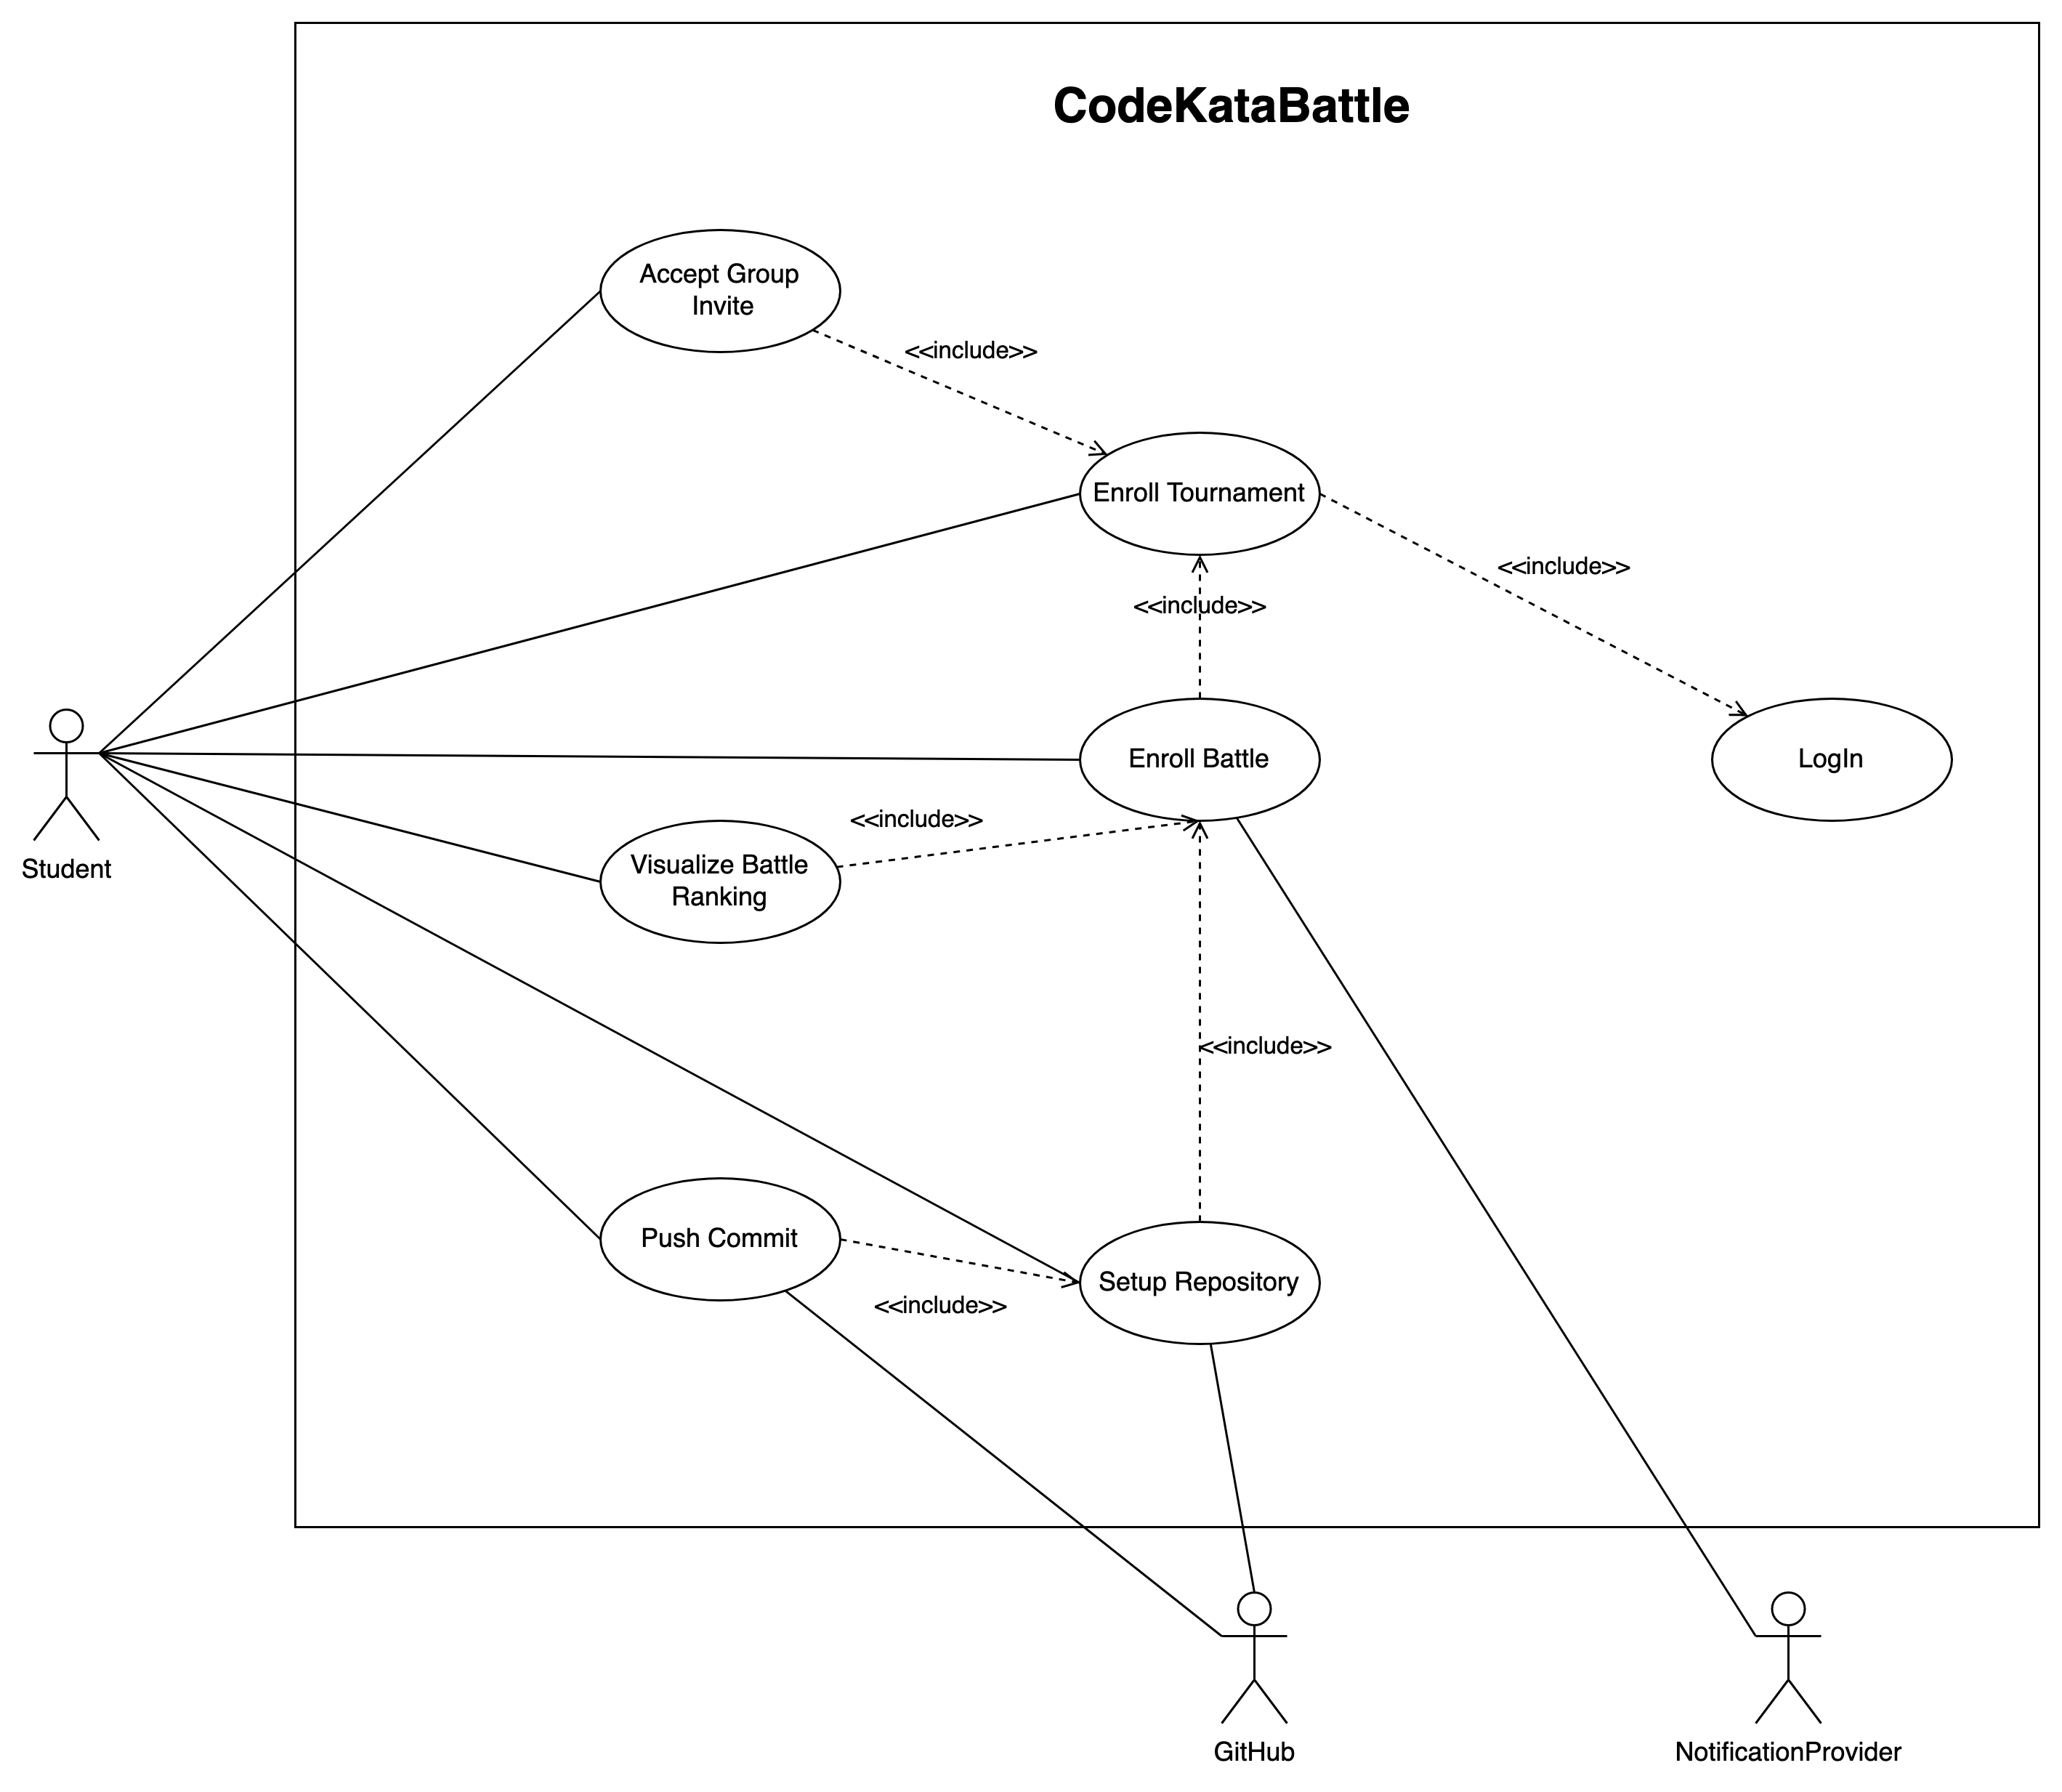
\includegraphics[scale = 0.45]{Images/UseCaseDiagrams/StudentUseCaseDiagram.png}\\
    \caption{Student}
\end{figure}
\begin{figure}[H]
    \centering
    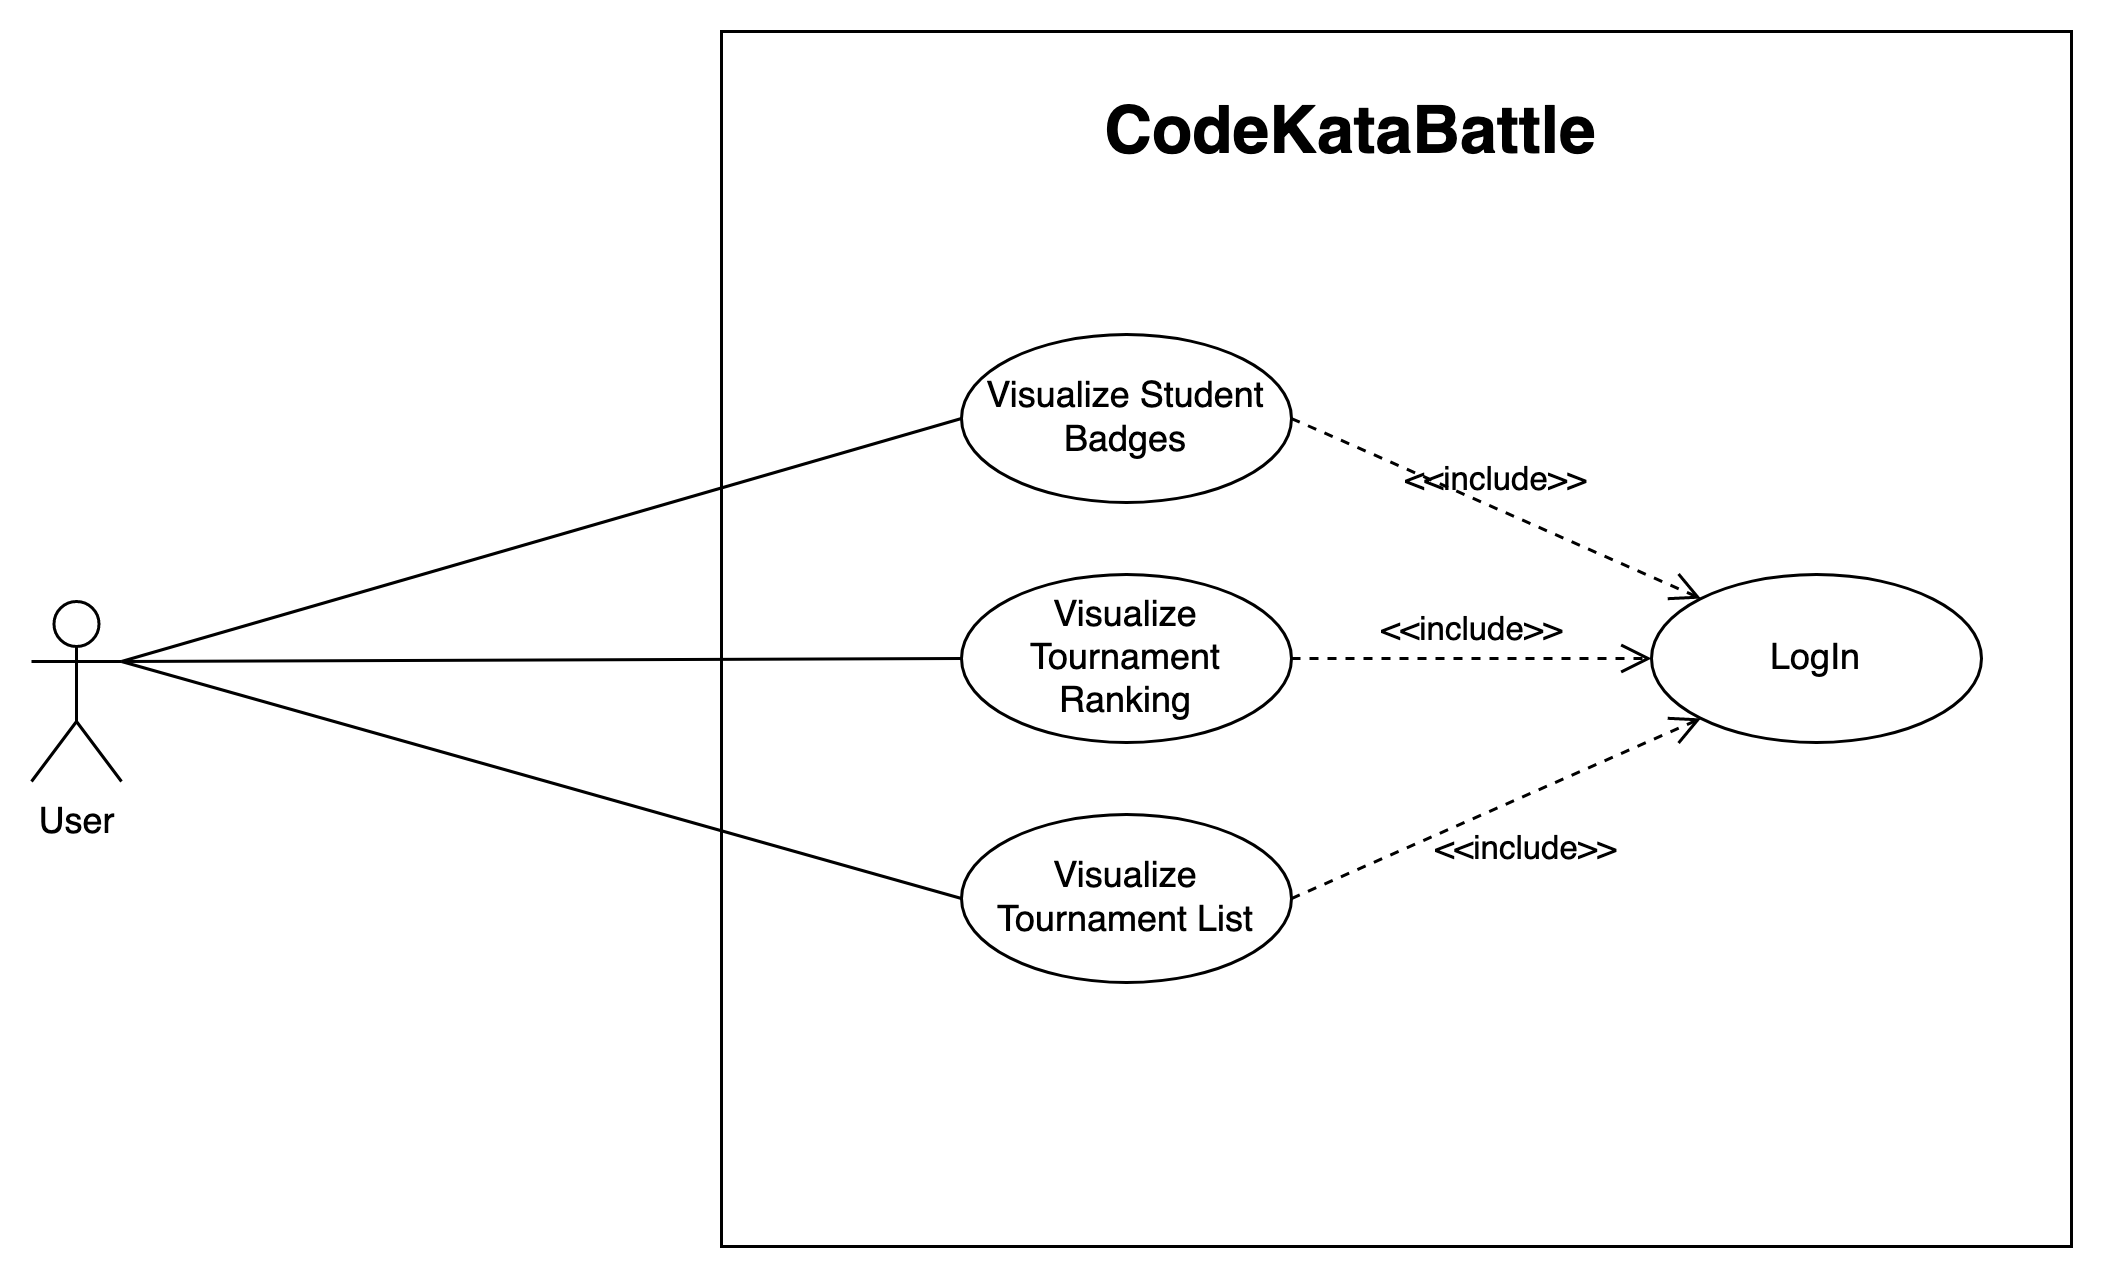
\includegraphics[scale = 0.45]{Images/UseCaseDiagrams/UserUseCaseDiagram.png}\\
    \caption{User}
\end{figure}
\begin{figure}[H]
    \centering
    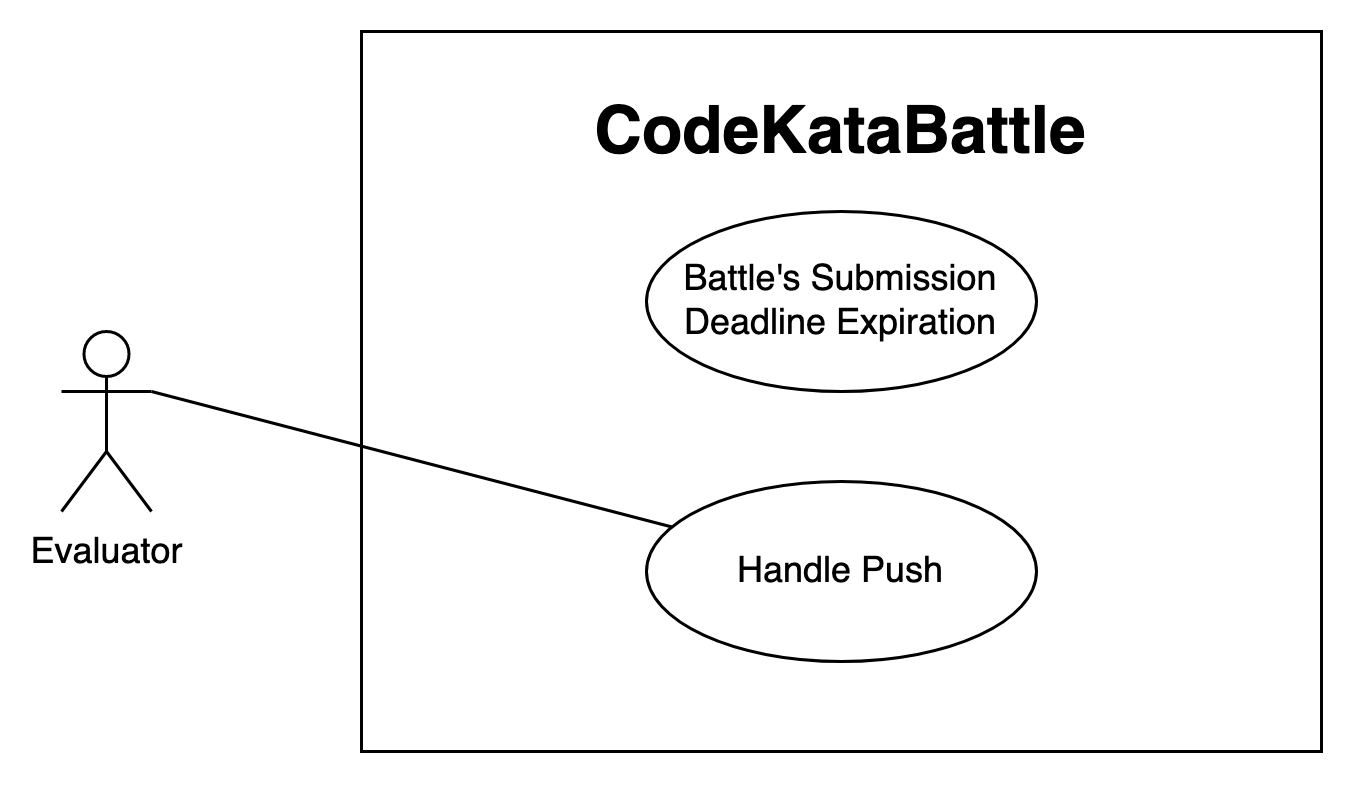
\includegraphics[scale = 0.45]{Images/UseCaseDiagrams/CKB_Autonomous_UseCaseDiagram.png}\\
    \caption{Evaluator}
\end{figure}

{\color{bluepoli}\rule{\linewidth}{0.1pt}}

\newpage
\subsection{Use Cases}

{\color{bluepoli}\rule{\linewidth}{0.1pt}}

\begin{xltabular}{\textwidth}{| l | X |}
\toprule
\multicolumn{2}{|c|}{StudentsSignUp}\\
\toprule
Participating Actors & Student, EmailService, CodeKataBattle\\ [1ex]
\hline
Entry Condition & True\\ [1ex]
\hline
Flow of Events & \begin{itemize}
		      \item 1. The Student opens the “Sign up” page
		      \item 2. CodeKataBattle shows the page to sign up
		      \item 3. The Student fills the required informations and clicks “Sign Up” button
		      \item 4. CodeKataBattle checks the information provided by the Student
		      \item 5. CodeKataBattle registers the Student
                \item 6. CodeKataBattle sends confirmation of signup and inform the Student to verify the account
                \item 7. CodeKataBattle sends a notification to verify the account through the EmailService
                \item 8. The Student verifies the account
                \item 9. CodeKataBattle activates the Student’s account
                \item 10. CodeKataBattle sends to the home page 
                \end{itemize} \\ [1ex]
\hline
Exit Condition & The Student successfully signed up and activated his account\\ [1ex]
\hline
Exceptions & The Student was already registered\\ [1ex]
\hline
\end{xltabular}
\begin{figure}[H]
\centering
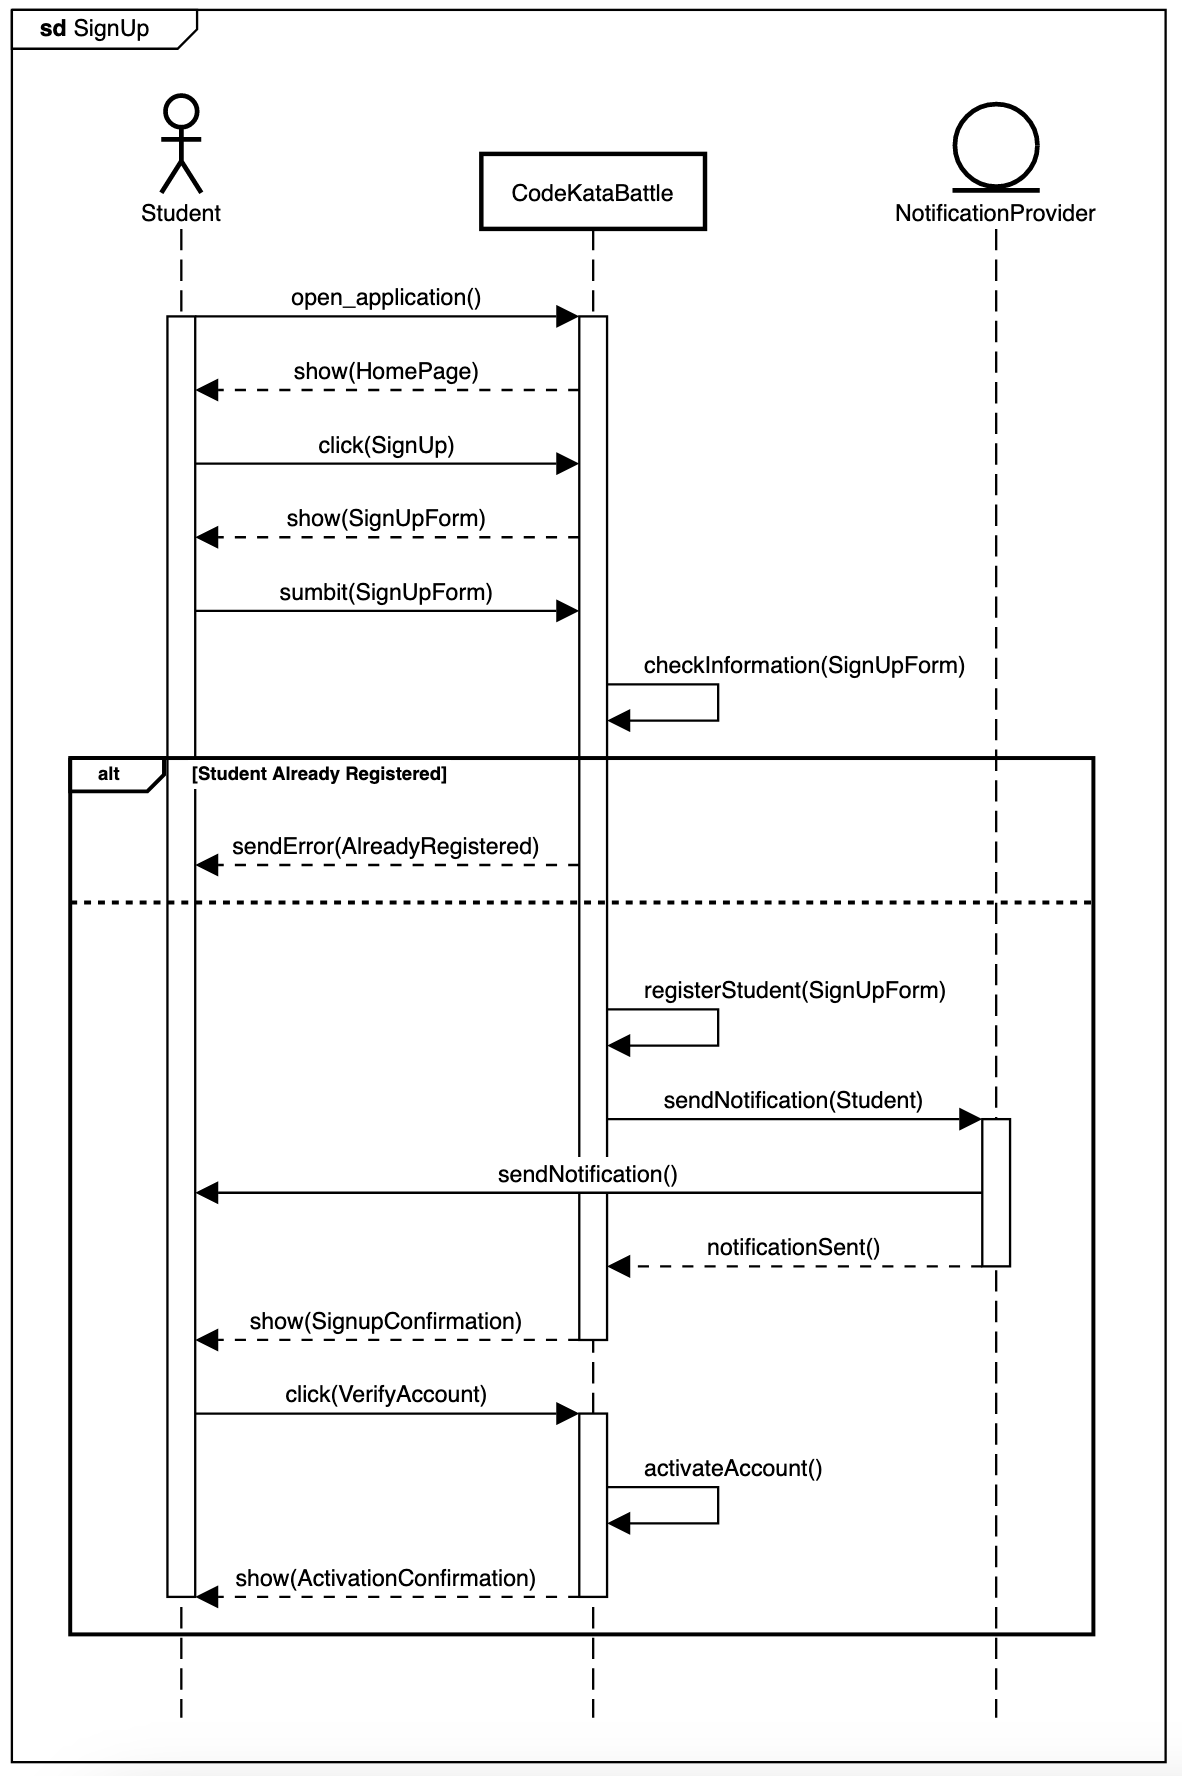
\includegraphics[scale = 0.45]{Images/SequenceDiagrams/StudentSignUpSeqDiagram.png}\\
\end{figure}
\newpage
\begin{xltabular}{\textwidth}{| l | X |}
\toprule
\multicolumn{2}{|c|}{EducatorsSignUp}\\
\toprule
Participating Actors & Educator, EmailService, CodeKataBattle\\ [1ex]
\hline
Entry Condition & True\\ [1ex]
\hline
Flow of Events & \begin{itemize}
		      \item 1. The Educator opens the “Sign up” page
		      \item 2. CodeKataBattle shows the page to sign up
		      \item 3. The Educator fills the required informations and clicks “Require An Educator Account” button
		      \item 4. CodeKataBattle shows the form to require an Educator account
		      \item 5. CodeKataBattle registers the Student
                \item 6. CodeKataBattle sends confirmation of signup and inform the Educator to verify the account
                \item 7. CodeKataBattle sends a notification to verify the account through the EmailService
                \item 8. The Educator verifies the account
                \item 9. CodeKataBattle activates the Educator’s account
                \item 10. CodeKataBattle sends to the home page 
                \end{itemize} \\ [1ex]
\hline
Exit Condition & The Educator successfully signed up and obtained an Educator account\\ [1ex]
\hline
Exceptions & The Educator was already registered\\ [1ex]
\hline
\end{xltabular}
\begin{figure}[H]
\centering
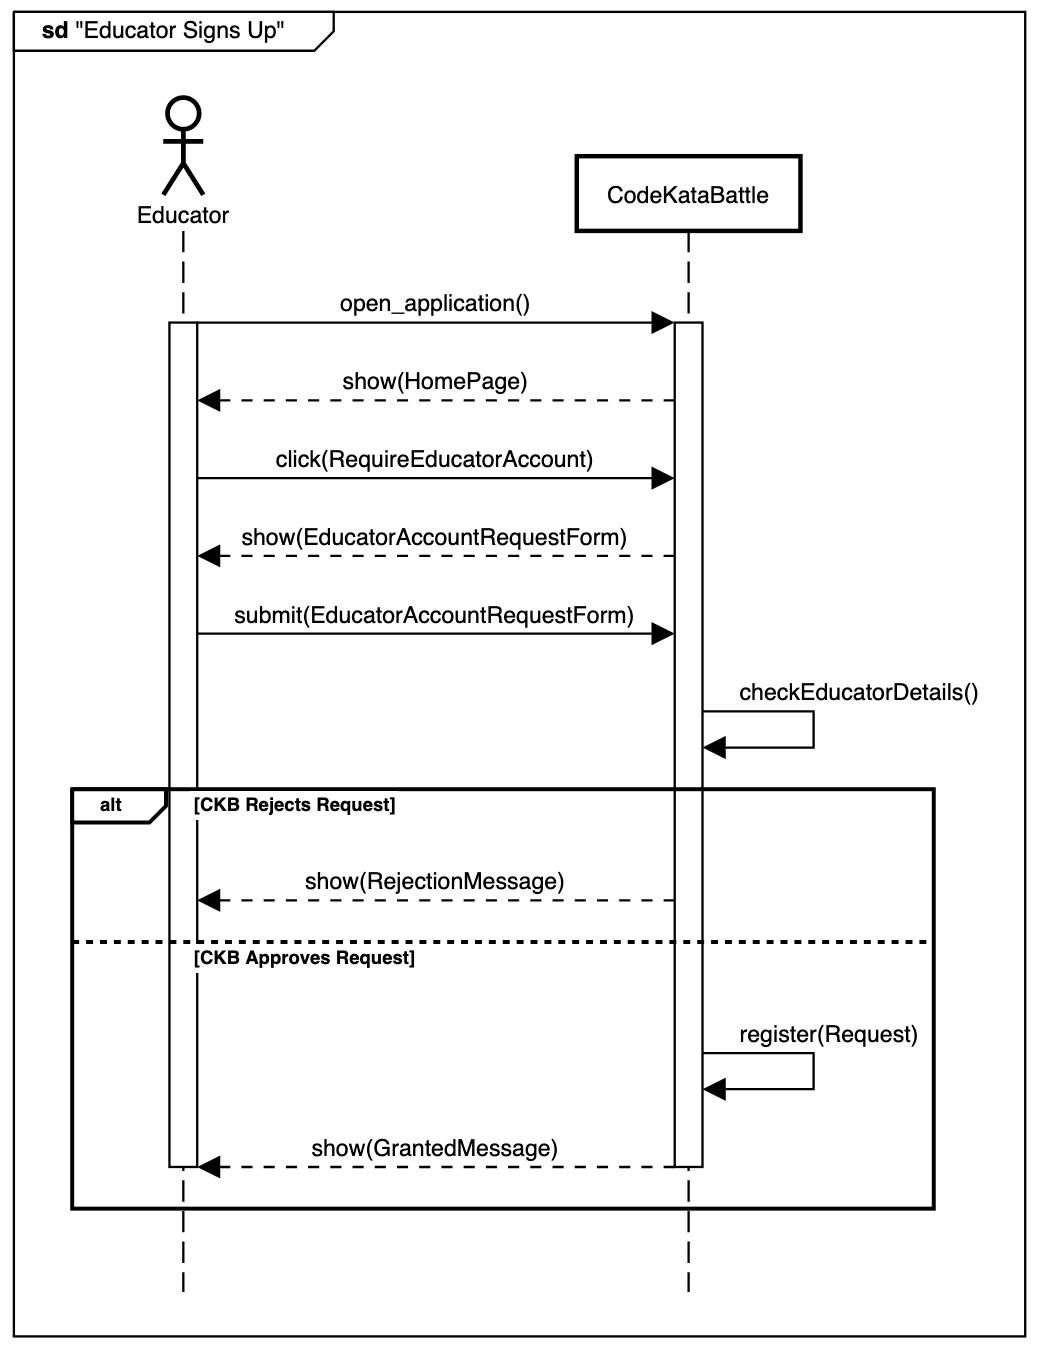
\includegraphics[scale = 0.45]{Images/SequenceDiagrams/EducatorSignUpSeqDiagram.png}\\
\end{figure}
\newpage
\begin{xltabular}{\textwidth}{| l | X |}
\toprule
\multicolumn{2}{|c|}{UserLogsIn}\\
\toprule
Participating Actors & User, CodeKataBattle\\ [1ex]
\hline
Entry Condition & User has an account\\ [1ex]
\hline
Flow of Events & \begin{itemize}
		      \item 1. The User opens CodeKataBattle
		      \item 2. The User clicks the “Log in” button
		      \item 3. CodeKataBattle shows the form to log in
		      \item 4. The User fills the required informations and clicks “Log in ” button
		      \item 5. CodeKataBattle verifies the credentials of the User
                \item 6. CodeKataBattle logs in the User 
                \end{itemize} \\ [1ex]
\hline
Exit Condition & The User successfully logged in\\ [1ex]
\hline
Exceptions & The User filled wrong credentials\\ [1ex]
\hline
\end{xltabular}
\begin{figure}[H]
    \centering
    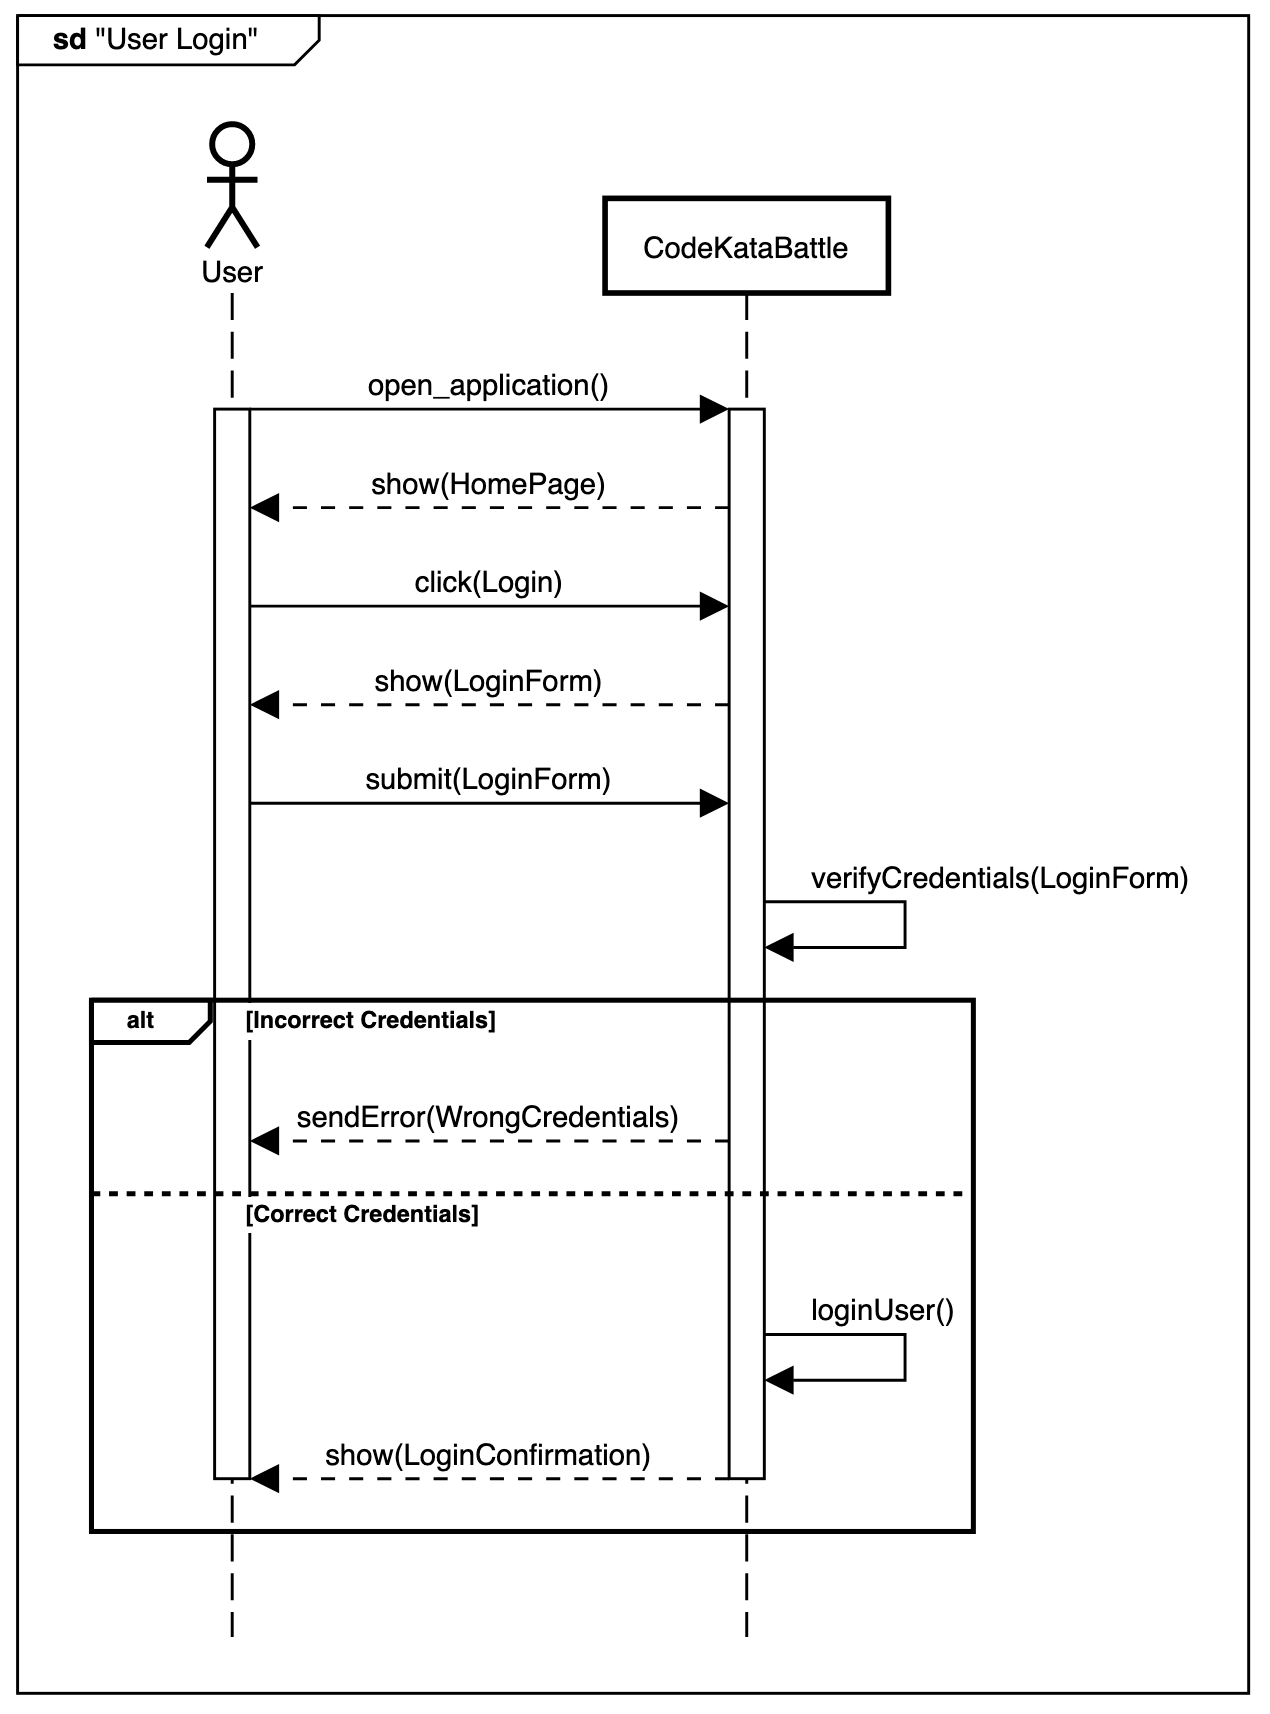
\includegraphics[scale = 0.45]{Images/SequenceDiagrams/LogInSeqDiagram.png}\\
\end{figure}
\newpage
\begin{xltabular}{\textwidth}{| l | X |}
\toprule
\multicolumn{2}{|c|}{CreateTournament}\\
\toprule
Participating Actors & Student, Educator, NotificationProvider, CodeKataBattle\\ [1ex]
\hline
Entry Condition & Educator is logged in\\ [1ex]
\hline
Flow of Events & \begin{itemize}
		      \item 1. The Educator clicks on the “Create a new Tournament” button
		      \item 2. CodeKataBattle shows the form to create a new Tournament
		      \item 3. The Educator chooses a subscription deadline and fills the correct field
		      \item 4. The Educator chooses whether to use Badges and eventually fills the relative fields
		      \item 5. The Educator chooses to which other colleagues grant the permission to manage the Tournament
                \item 6. The Educator clicks the “Create” button
                \item 7. CodeKataBattle creates the Tournament
                \item 8. CodeKataBattle notifies through the NotificationProvider all the Students subscribed to the platform of the creation of the Tournament
                \end{itemize} \\ [1ex]
\hline
Exit Condition & The Educator successfully created a new Tournament and CodeKataBattle successfully notifies all the subscribed Students\\ [1ex]
\hline
Exceptions & None\\ [1ex]
\hline
\end{xltabular}
\begin{figure}[H]
    \centering
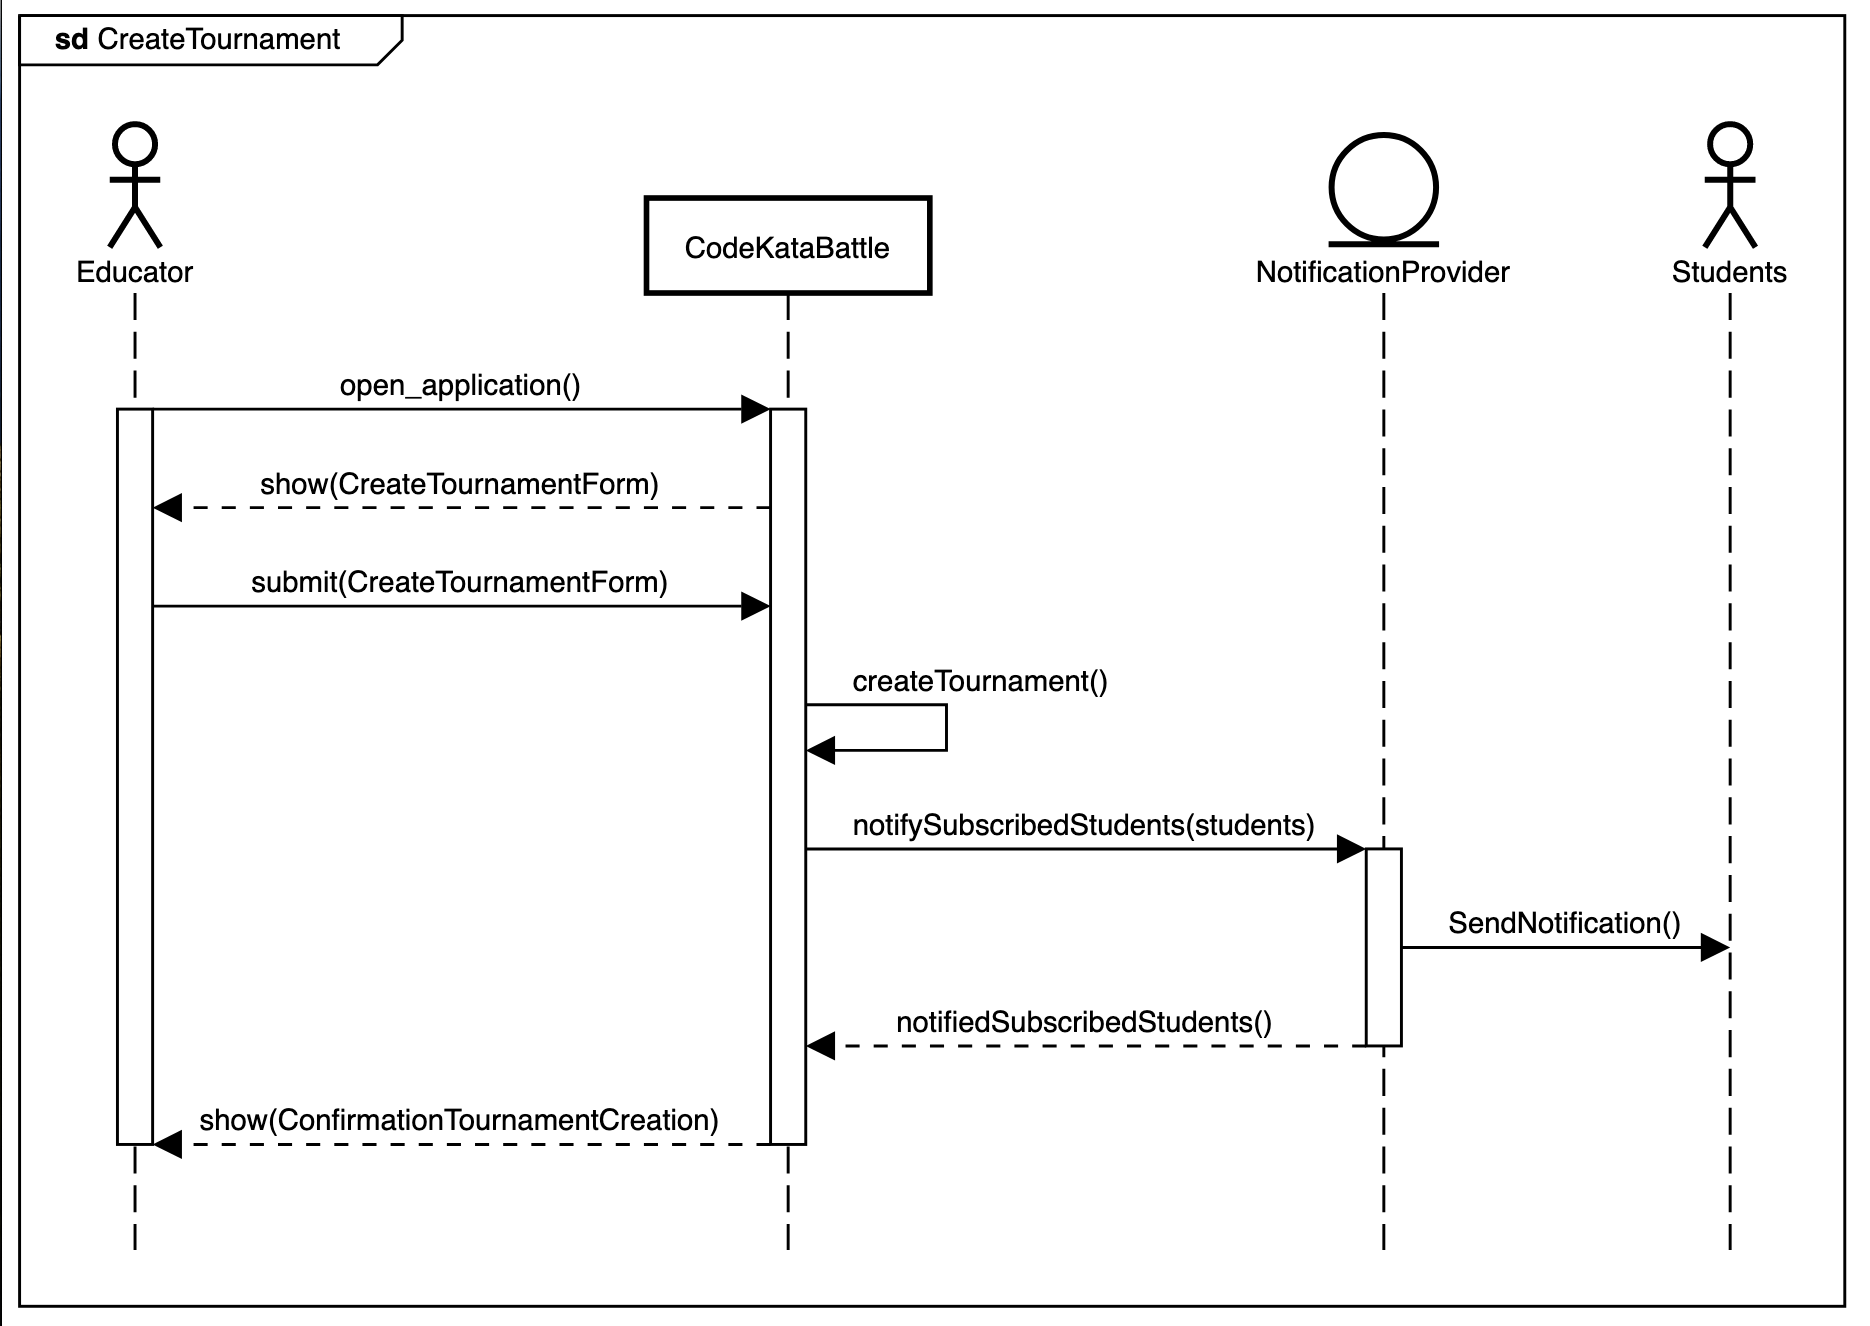
\includegraphics[scale = 0.45]{Images/SequenceDiagrams/CreateTournamentSeqDiagram.png}\\
\end{figure}
\newpage
\begin{xltabular}{\textwidth}{| l | X |}
\toprule
\multicolumn{2}{|c|}{EducatorGrantsPermissionToColleagues}\\
\toprule
Participating Actors & Educator, CodeKataBattle\\ [1ex]
\hline
Entry Condition & The Educator is creating a Tournament\\ [1ex]
\hline
Flow of Events & \begin{itemize}
		      \item 1. CodeKataBattle shows the Tournament’s details
		      \item 2. The Educator clicks on the “Grant Permissions” button
		      \item 3. CodeKataBattle shows the page to handle permissions for the Tournament
		      \item 4. The Educator clicks on the “Add Educator” button
		      \item 5. CodeKataBattle shows a form to grant other Educators permissions on the Tournament
                \item 6. The Educator fills the requested information and clicks “Confirm” button
                \item 7. CodeKataBattle recognizes the newly authorized Students
                \end{itemize} \\ [1ex]
\hline
Exit Condition & The Educator successfully granted permission to manage the Tournament to another Educator\\ [1ex]
\hline
Exceptions & None\\ [1ex]
\hline
\end{xltabular}
\begin{figure}[H]
    \centering
    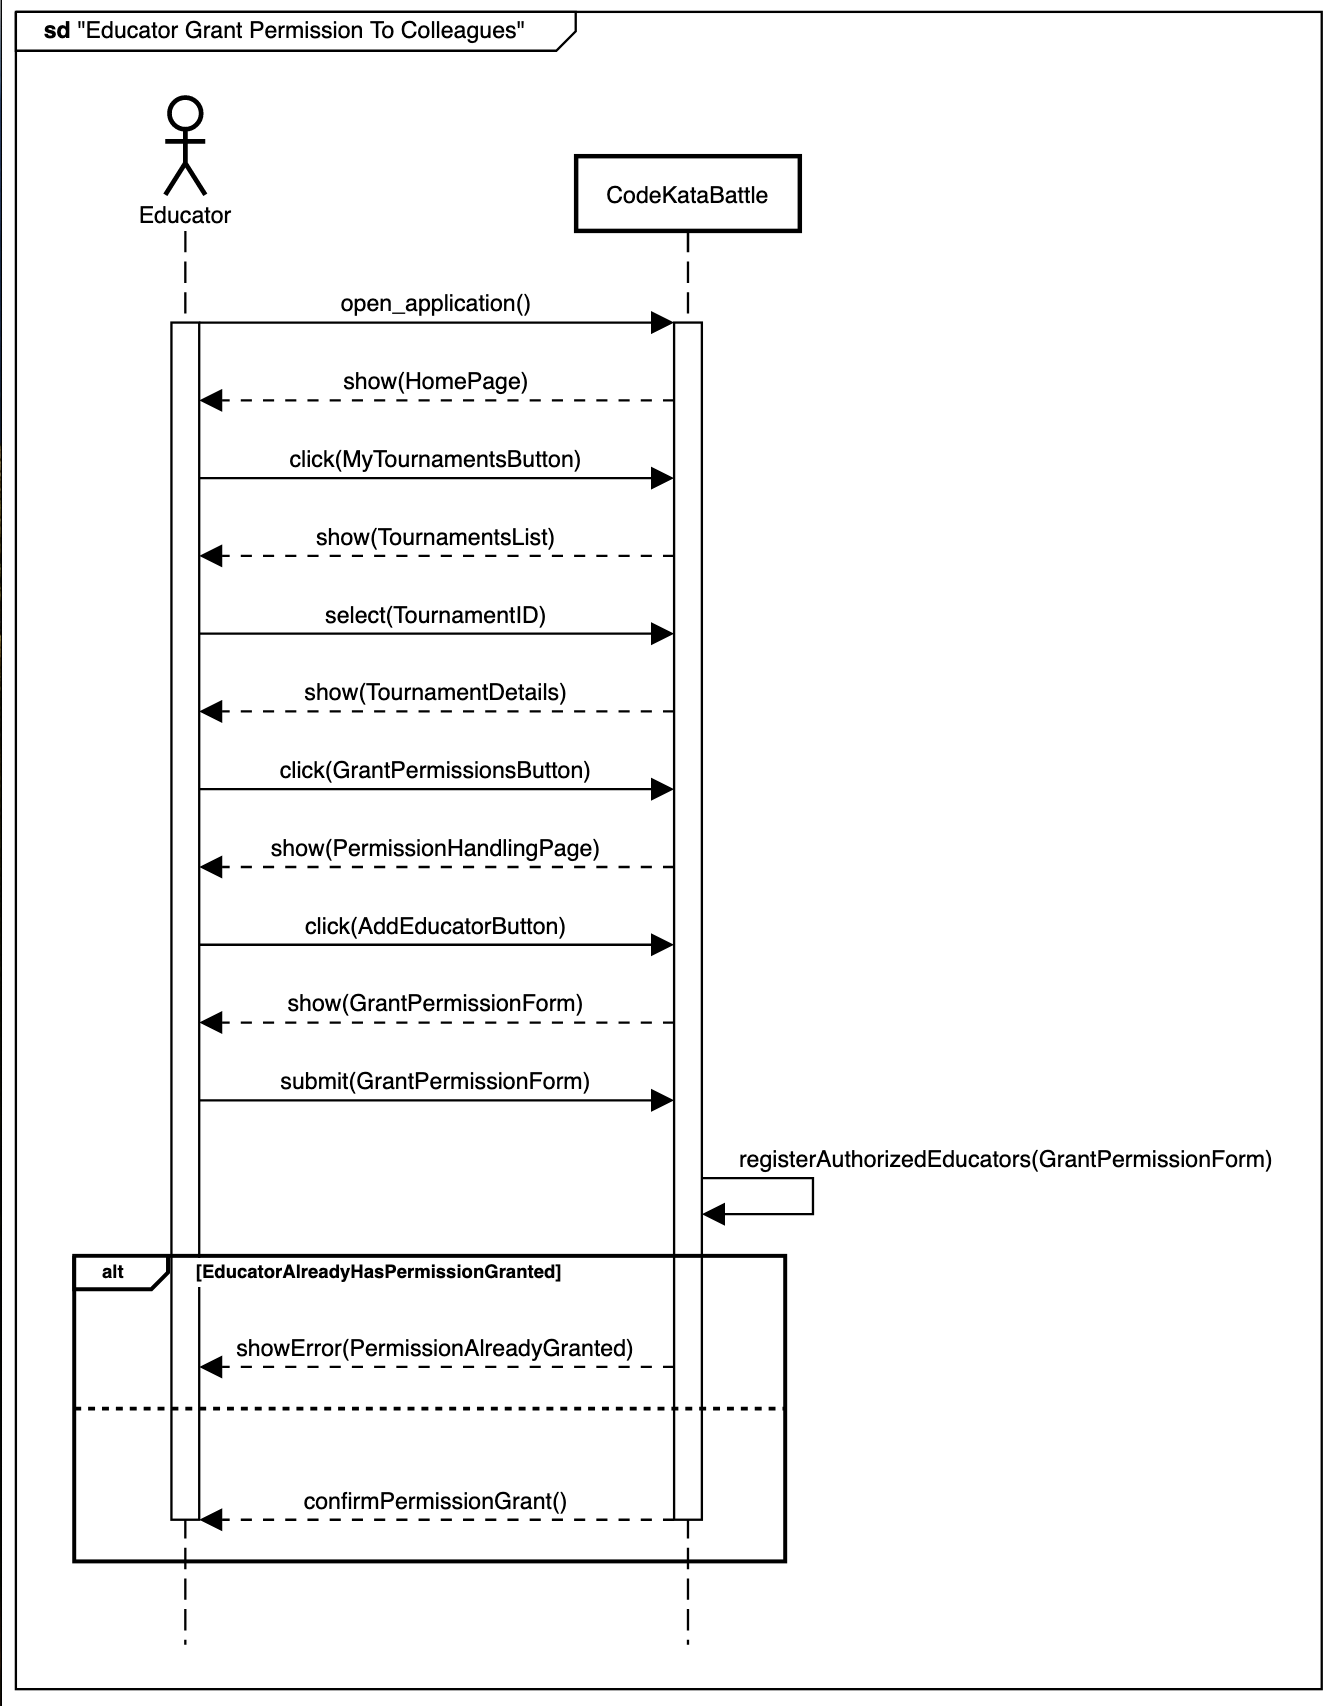
\includegraphics[scale = 0.45]{Images/SequenceDiagrams/EducatorGrantsPermissionCollagueSeqDiagram.png}\\
\end{figure}
\newpage
\begin{xltabular}{\textwidth}{| l | X |}
\toprule
\multicolumn{2}{|c|}{CreateBattle}\\
\toprule
Participating Actors & Student, Educator, NotificationProvider, CodeKataBattle\\ [1ex]
\hline
Entry Condition & The Educator is logged in and is granted the permission to manage a Tournament\\ [1ex]
\hline
Flow of Events & \begin{itemize}
		      \item 1. The Educator clicks on the “My Tournaments” button
		      \item 2. CodeKataBattle shows the list of the Tournaments that the Educator is allowed to manage
		      \item 3. The Educator clicks on a Tournament
		      \item 4. CodeKataBattle shows the Tournament’s details
		      \item 5. The Educator clicks on “Create a new Battle” button
                \item 6. CodeKataBattle shows the form to create a new Battle
                \item 7. The Educator uploads the problem
                \item 8. The Educator uploads the CodeKata
                \item 9. The Educator fills the minimum and maximum number of Students per team
                \item 10. The Educator fills the minimum and maximum number of Students per team
                \item 11. The Educator chooses a registration deadline 
                \item 12. The Educator chooses a submission deadline
                \item 13. The Educator chooses the scoring configuration
                \item 14. The Educator clicks the “Create” button
                \item 15. CodeKataBattle creates the Battle
                \item 16. CodeKataBattle notifies through the NotificationProvider all the Students subscribed to the Tournament of the creation of the Battle
                \end{itemize} \\ [1ex]
\hline
Exit Condition & The Educator successfully created a new Battle in a Tournament and CodeKataBattle successfully notifies all the Students subscribed to the Tournament\\ [1ex]
\hline
Exceptions & None\\ [1ex]
\hline
\end{xltabular}
\begin{figure}[H]
    \centering
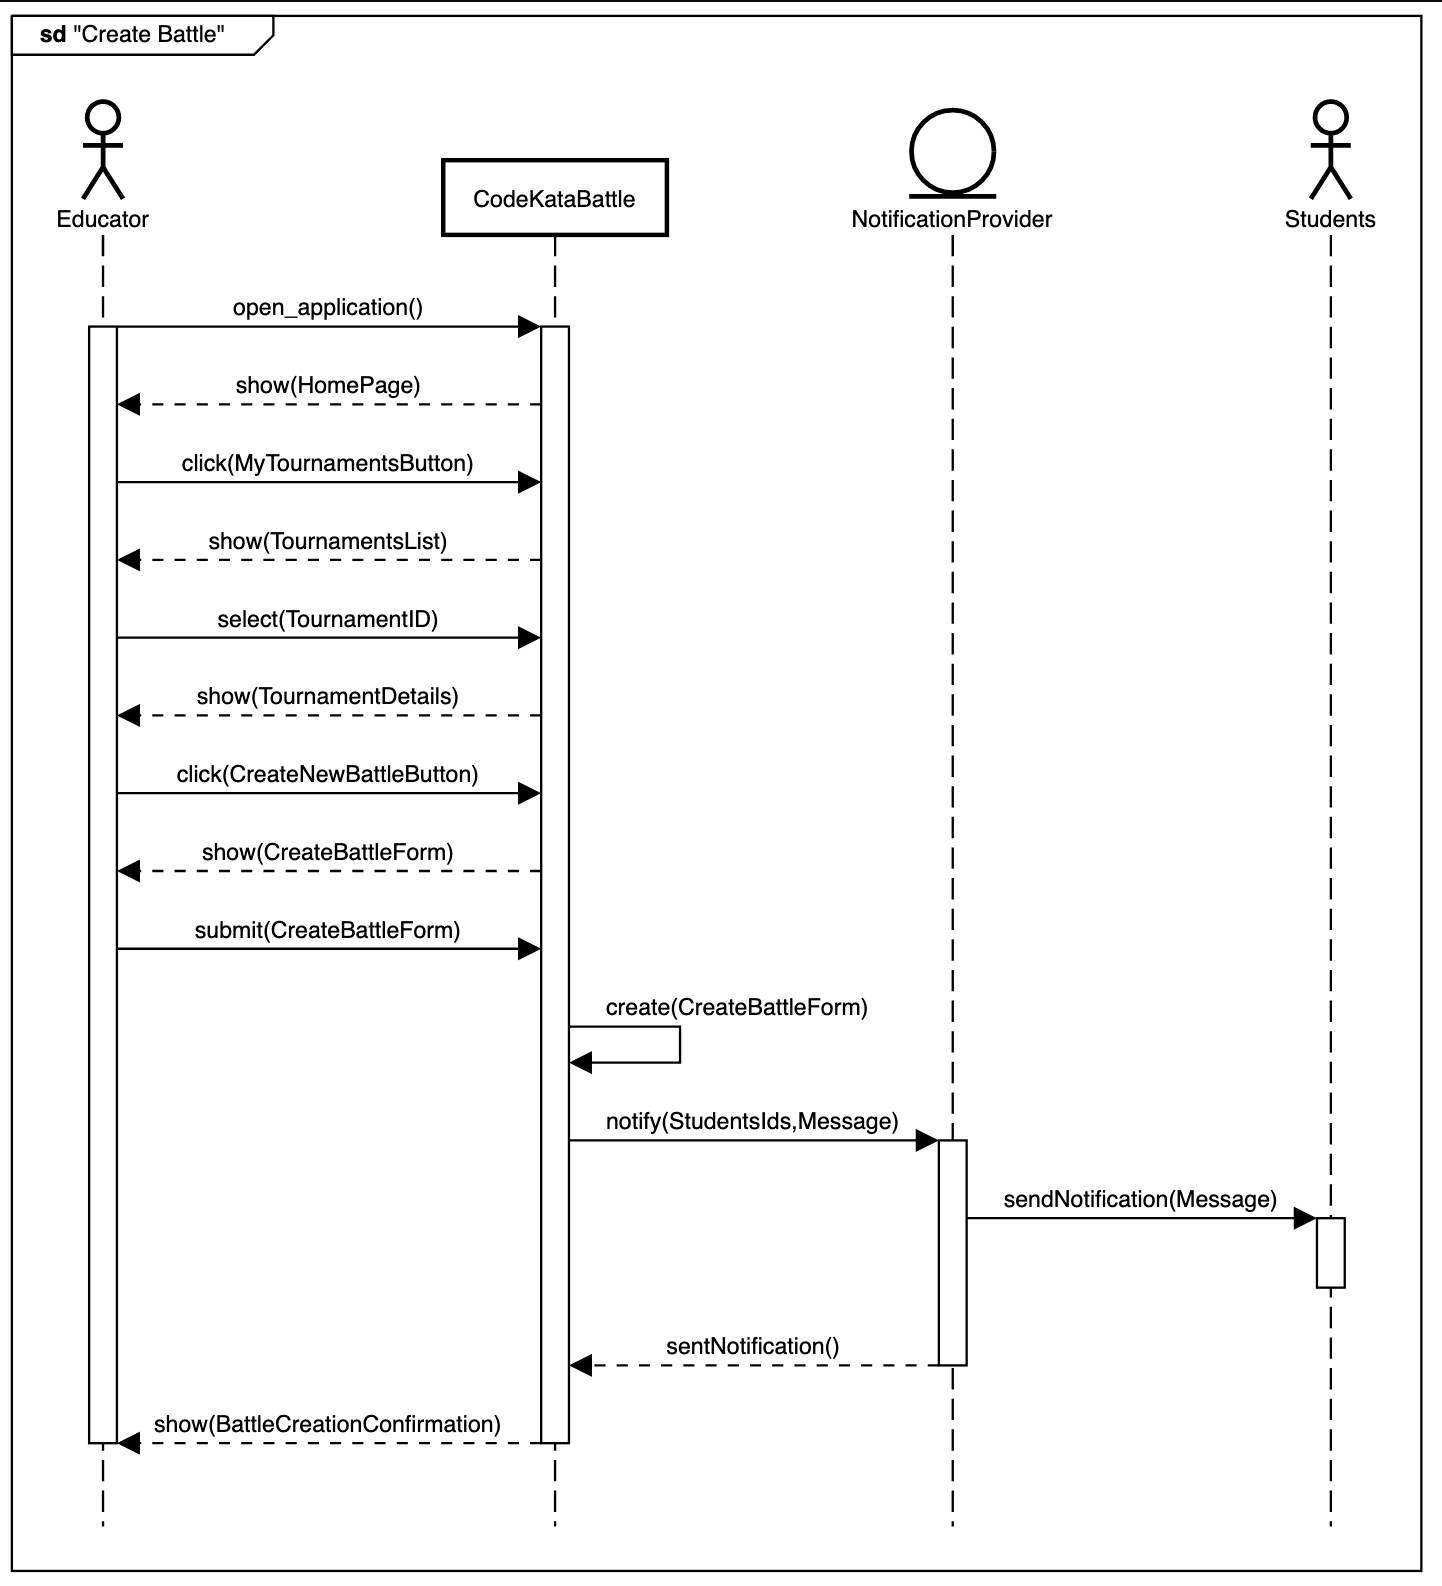
\includegraphics[scale = 0.45]{Images/SequenceDiagrams/EducatorCreatesBattleSeqDiagram.png}\\
\end{figure}
\newpage
\begin{xltabular}{\textwidth}{| l | X |}
\toprule
\multicolumn{2}{|c|}{StudentEnrollsInTournament}\\
\toprule
Participating Actors & Student, CodeKataBattle\\ [1ex]
\hline
Entry Condition & The Student is logged in and at least a Tournament has been created\\ [1ex]
\hline
Flow of Events & \begin{itemize}
		      \item 1. The Student clicks on the “All Tournaments” button
		      \item 2. CodeKataBattle shows the list of all the Tournaments
		      \item 3. The Student clicks on a Tournament
		      \item 4. CodeKataBattle shows the Tournament’s details
		      \item 5. The Student clicks on “Subscribe” button
                \item 6. CodeKataBattle performs the Student’s subscription
                \end{itemize} \\ [1ex]
\hline
Exit Condition & The Student successfully subscribed to the Tournament\\ [1ex]
\hline
Exceptions & The subscription deadline for the chosen Tournament is expired\\ [1ex]
\hline
\end{xltabular}
\begin{figure}[H]
    \centering
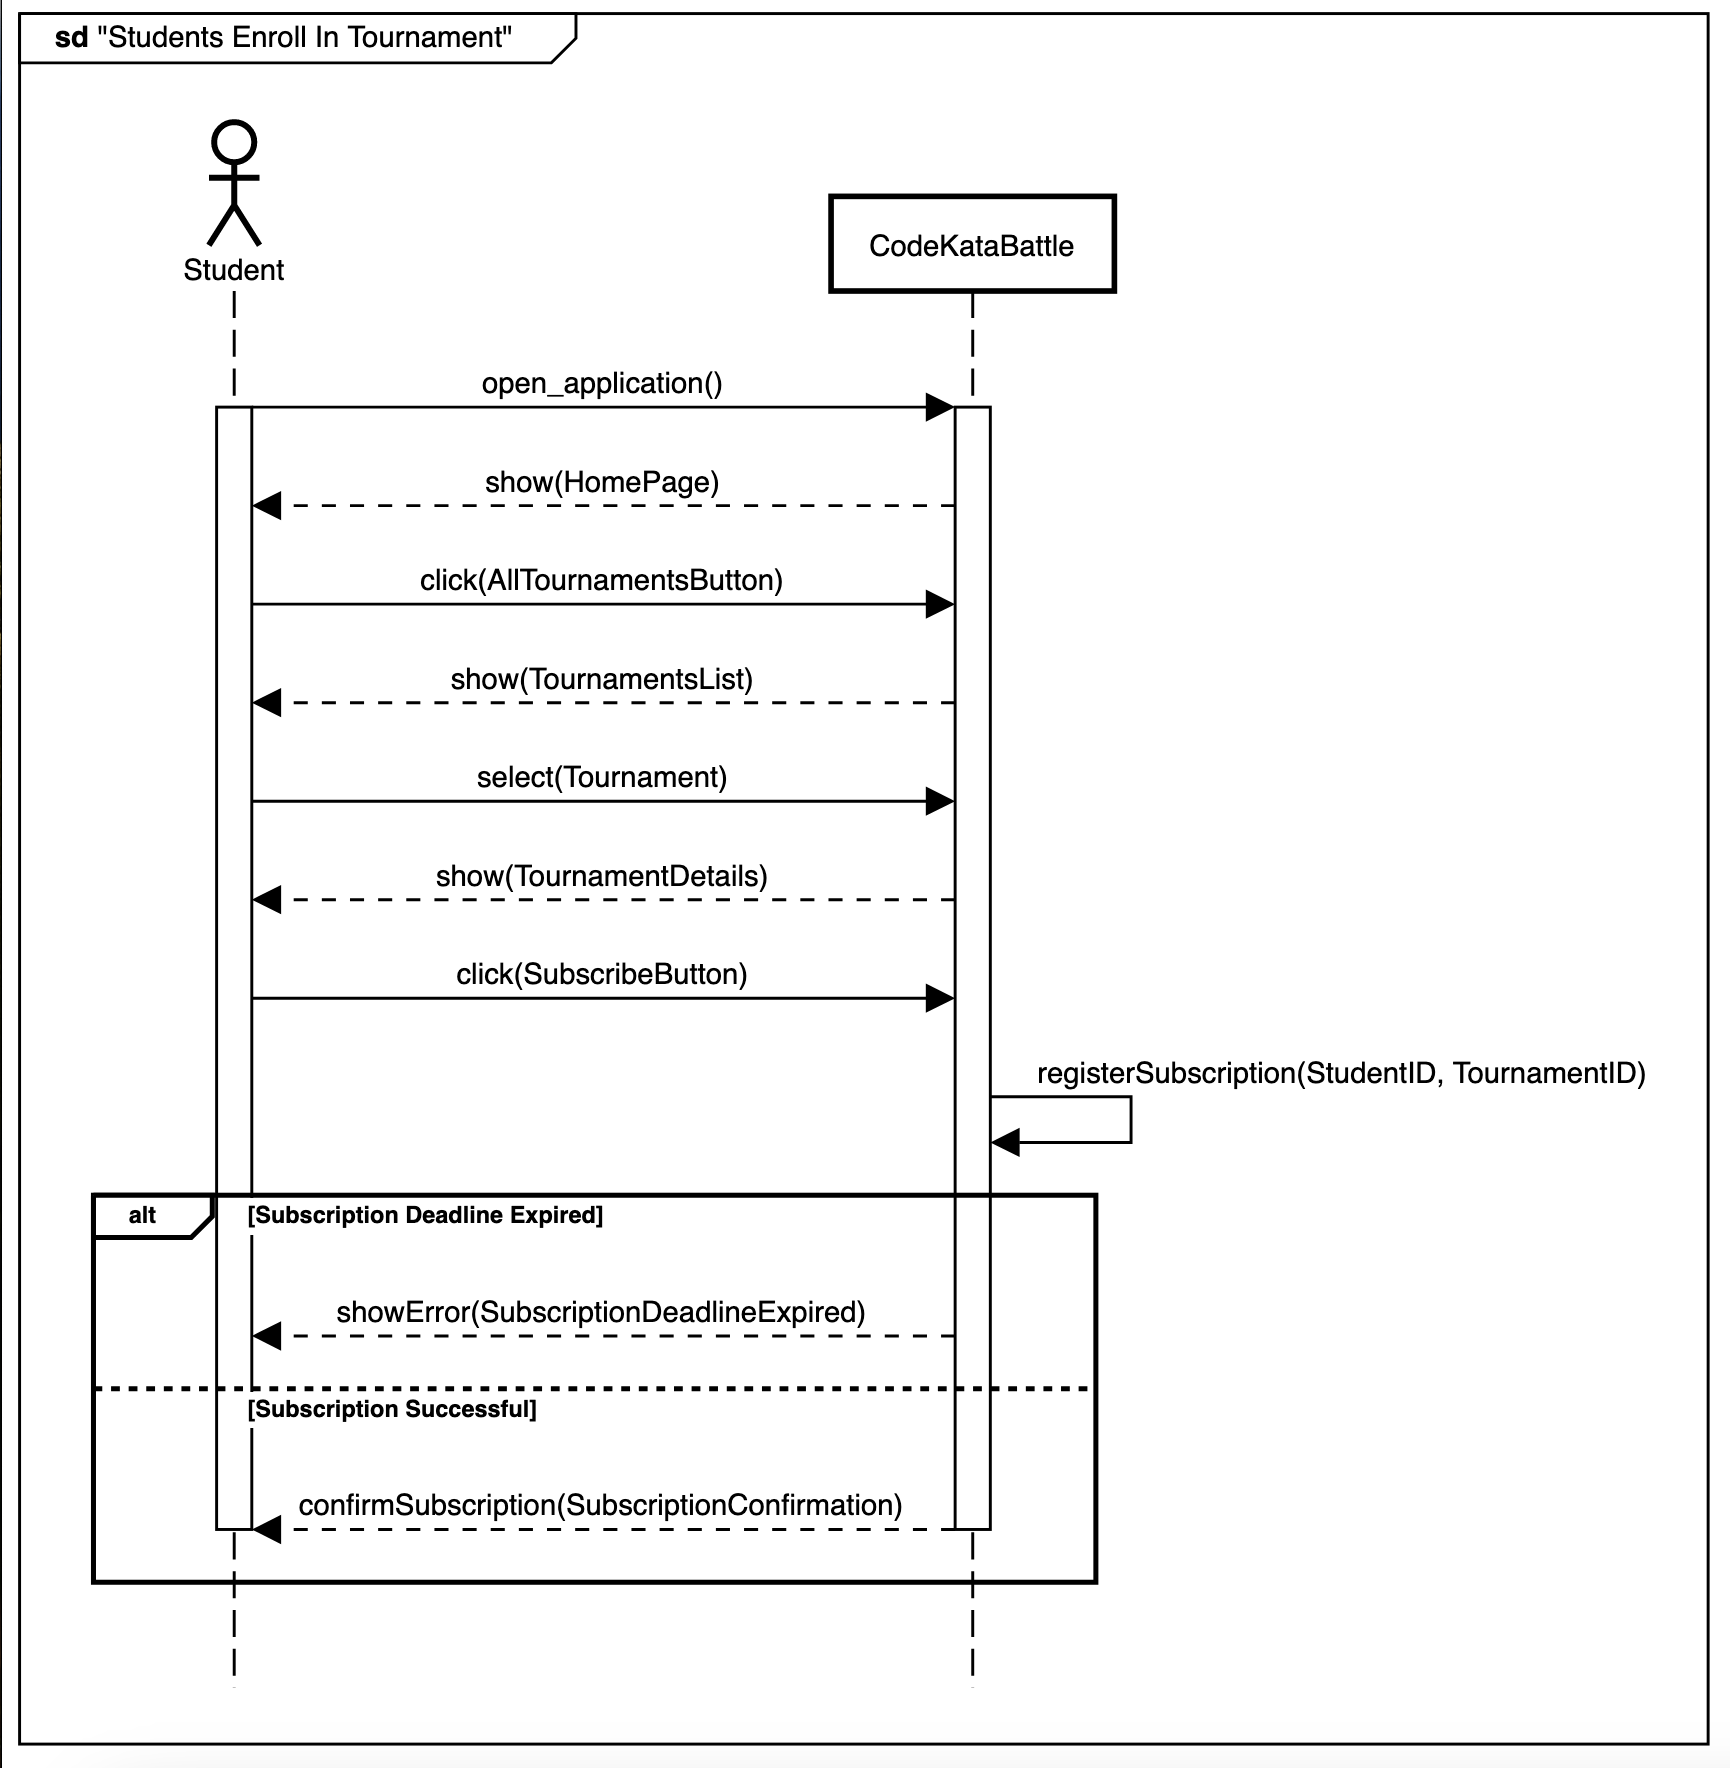
\includegraphics[scale = 0.45]{Images/SequenceDiagrams/StudentEnrollsInTournamentSeqDiagram.png}\\
\end{figure}

\newpage
\begin{xltabular}{\textwidth}{| l | X |}
\toprule
\multicolumn{2}{|c|}{StudentEnrollsInBattle}\\
\toprule
Participating Actors & Student, CodeKataBattle\\ [1ex]
\hline
Entry Condition & Student is logged in and subscribed to the Battle’s Tournament\\ [1ex]
\hline
Flow of Events & \begin{itemize}
		      \item 1. The Student clicks on the “My Tournaments” button
		      \item 2. CodeKataBattle shows the list of the Tournaments the Student is enrolled in
		      \item 3. The Student clicks on a Tournament
		      \item 4. CodeKataBattle shows the Tournament’s details
		      \item 5. The Student clicks on the Battle he wants to enroll in
                \item 6. CodeKataBattle shows the Battle’s details
                \item 7. The Student clicks on the “Subscribe” button
                \item 8. CodeKataBattle shows the form to specify the group composition
                \item 9. The Student makes his choice and invites other Students
                \item 10. CodeKataBattle performs the Student’s subscription
                \end{itemize} \\ [1ex]
\hline
Exit Condition & The Student successfully subscribed to the Battle and eventually invites other Students\\ [1ex]
\hline
Exceptions & \begin{itemize}
                \item The subscription deadline for the chosen Battle is expired
                \item The number of Students in the group is invalid
                \item Some Students who are being invited are not enrolled in the Tournament
                \end{itemize} \\ [1ex]
\hline
\end{xltabular}
\begin{figure}[H]
    \centering
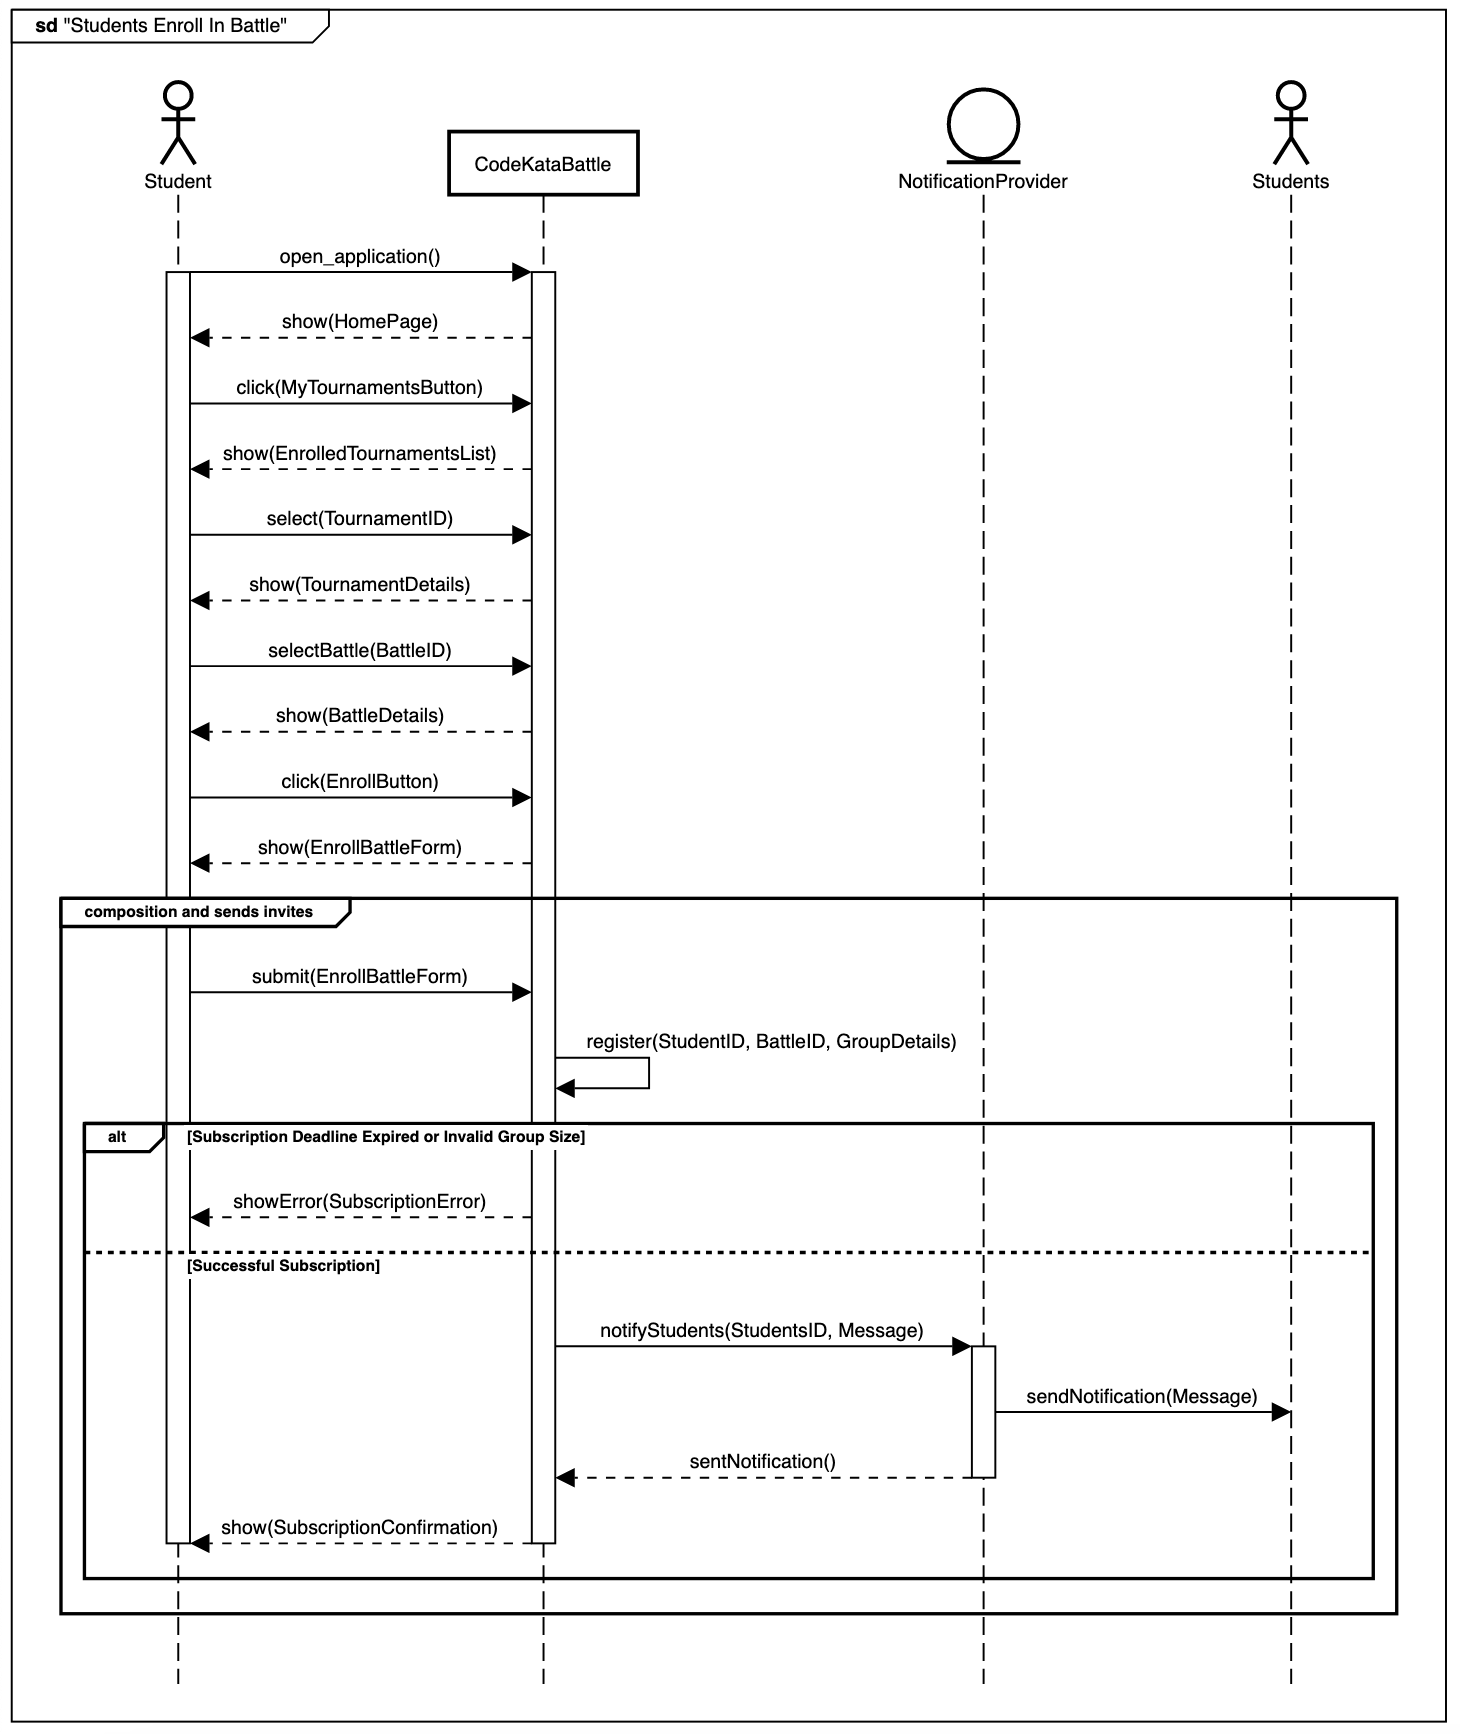
\includegraphics[scale = 0.45]{Images/SequenceDiagrams/StudentEnrollsInBattleSeqDiagram.png}\\
\end{figure}
\newpage
\begin{xltabular}{\textwidth}{| l | X |}
\toprule
\multicolumn{2}{|c|}{StudentAcceptsBattleInvitation}\\
\toprule
Participating Actors & Student, CodeKataBattle\\ [1ex]
\hline
Entry Condition & Student received an invite to join a group for a Battle\\ [1ex]
\hline
Flow of Events & \begin{itemize}
		      \item 1. The Student clicks on the “Join Group” button of the received invite 
		      \item 2. CodeKataBattle registers the Student’s subscription to the Battle and the enrollment in the group
                \end{itemize} \\ [1ex]
\hline
Exit Condition & The Student successfully subscribed to the Battle and joined the team of the Student who invited him\\ [1ex]
\hline
Exceptions & The Students had already accepted the invite \\ [1ex]
\hline
\end{xltabular}
\begin{figure}[H]
\centering
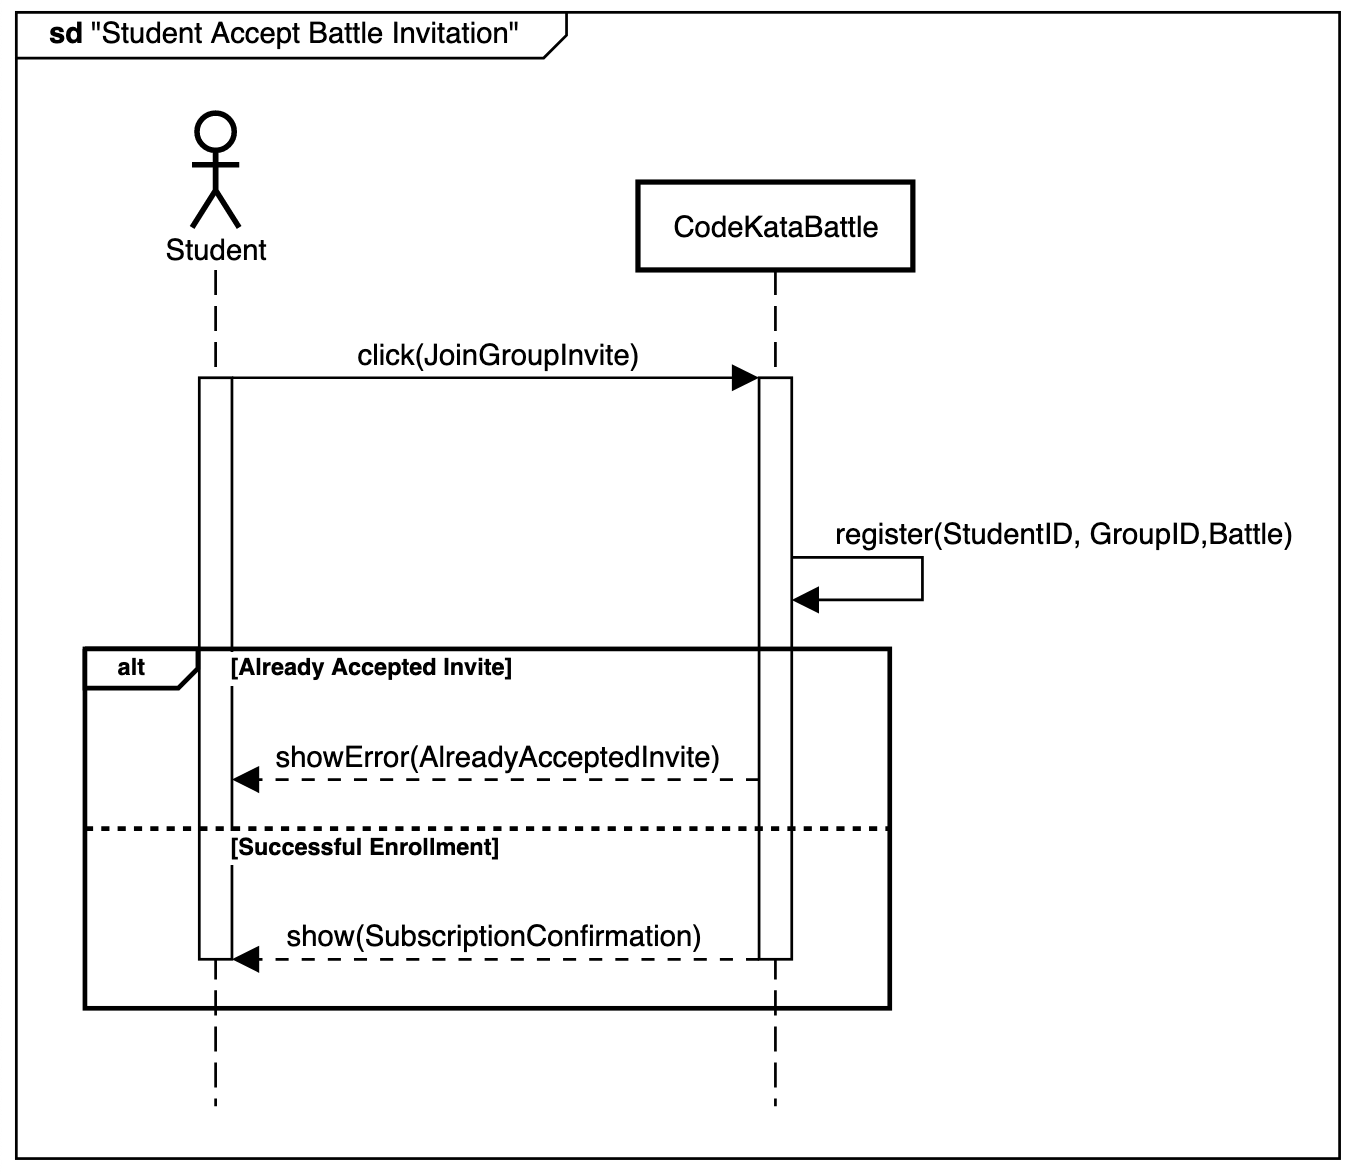
\includegraphics[scale = 0.45]{Images/SequenceDiagrams/StudentAcceptsInviteSeqDiagram.png}\\
\end{figure}
\newpage
\begin{xltabular}{\textwidth}{| l | X |}
\toprule
\multicolumn{2}{|c|}{BattlesSubscriptionDeadlineExpiration}\\
\toprule
Participating Actors & GitHub, CodeKataBattle\\ [1ex]
\hline
Entry Condition & A Battle's subscription deadline has reached its expiration point\\ [1ex]
\hline
Flow of Events & \begin{itemize}
		      \item 1. CodeKataBattle closes Battle’s subscription stage
		      \item 2. CodeKataBattle creates the Battle’s GitHub repository
                \item 3. CodeKataBattle pushes the CodeKata to the newly created repository
                \item 4. CodeKataBattle shares with them the link to the GitHub repository
                \item 5. CodeKataBattle starts registering submissions for the subscribed members
                \end{itemize} \\ [1ex]
\hline
Exit Condition & The Battle's subscription is closed, preventing further participation after the deadline and the GitHub repository associated with the Battle has been created\\ [1ex]
\hline
Exceptions & The GitHub API call fails \\ [1ex]
\hline
\end{xltabular}
\begin{figure}[H]
\centering
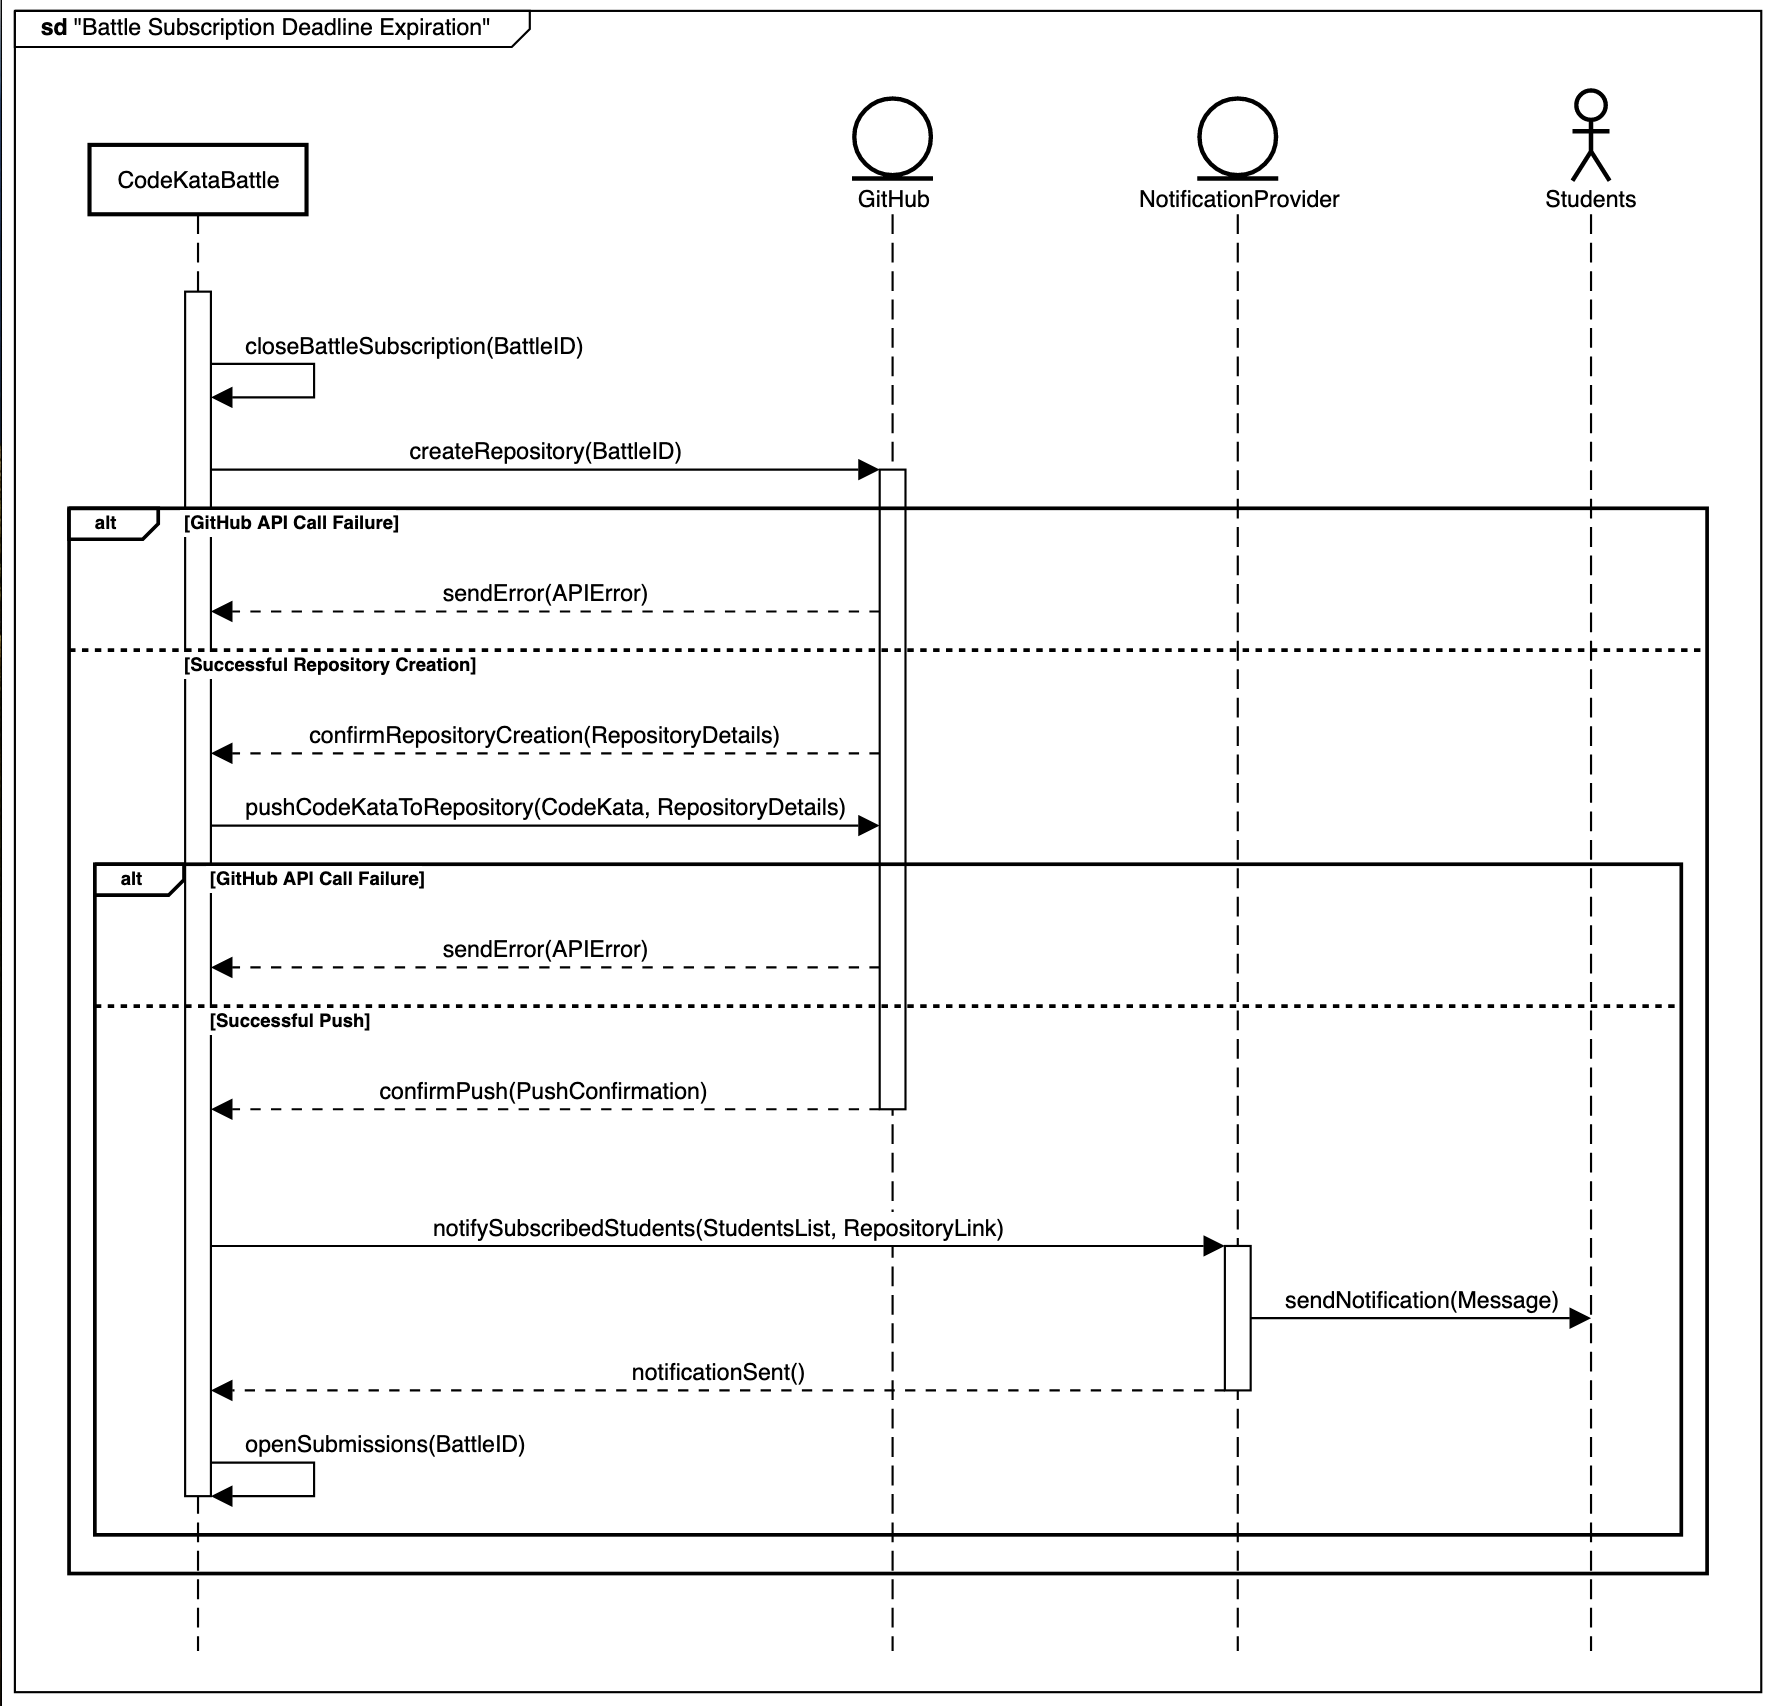
\includegraphics[scale = 0.45]{Images/SequenceDiagrams/BattleSubscDeadlineExpiredSeqDiagram.png}\\
\end{figure}
\newpage
\begin{xltabular}{\textwidth}{| l | X |}
\toprule
\multicolumn{2}{|c|}{StudentSetsUpTheRepository}\\
\toprule
Participating Actors & GitHub, Student\\ [1ex]
\hline
Entry Condition & The Student is enrolled in the Battle and has a GitHub account\\ [1ex]
\hline
Flow of Events & \begin{itemize}
		      \item 1. The Student opens the link to the repository
		      \item 2. The Student forks the repository
                \item 3. The Student adds his team members as collaborators in the repository
                \item 4. The Student sets up the “GitHub Action”
                \end{itemize} \\ [1ex]
\hline
Exit Condition & The Student successfully forked the Battle’s GitHub repository and set up the GitHub Action\\ [1ex]
\hline
Exceptions & The GitHub website is temporarly unavailable \\ [1ex]
\hline
\end{xltabular}
\begin{figure}[H]
    \centering
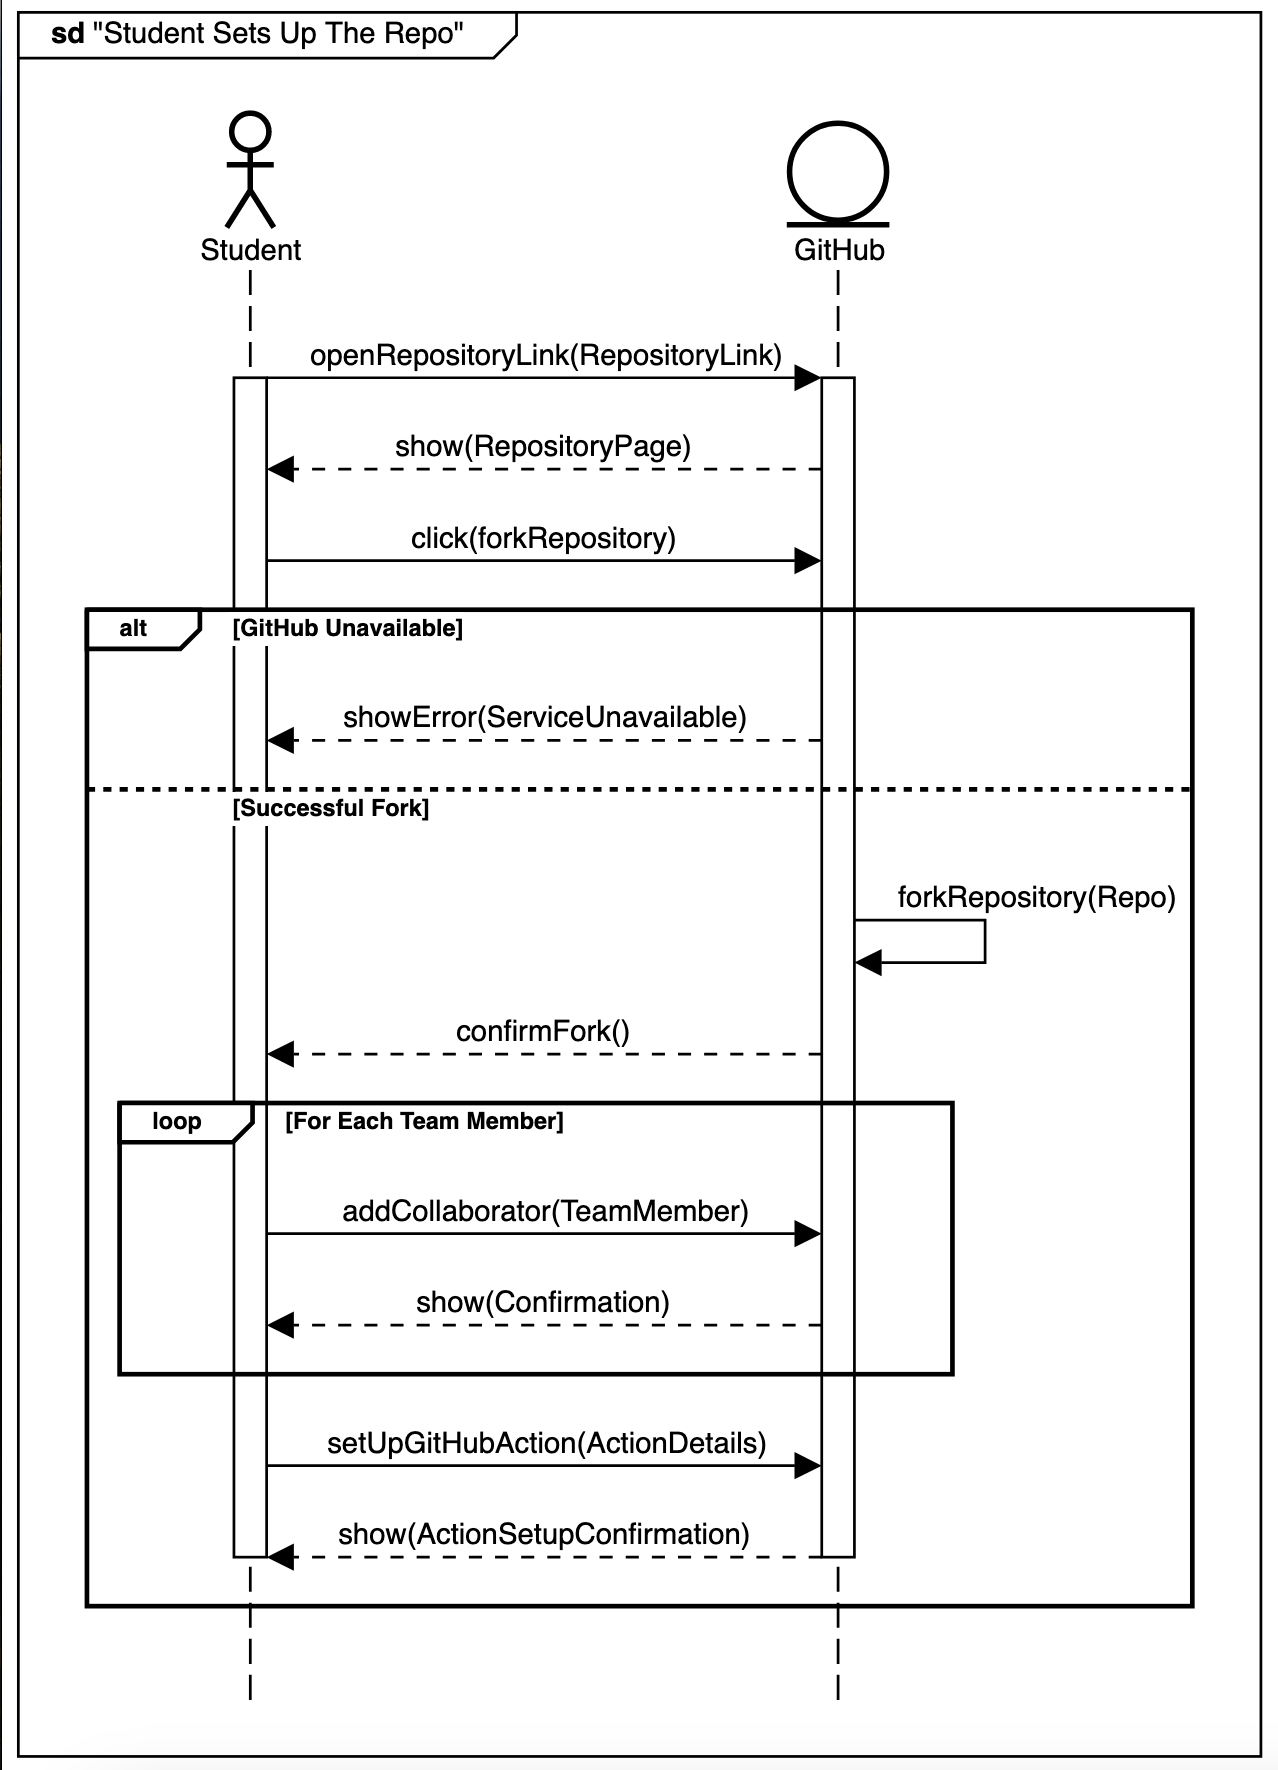
\includegraphics[scale = 0.45]{Images/SequenceDiagrams/StudentSetUpRepoSeqDiagram.png}\\
\end{figure}
\newpage
\begin{xltabular}{\textwidth}{| l | X |}
\toprule
\multicolumn{2}{|c|}{CodeKataHandlesStudentsPush}\\
\toprule
Participating Actors & GitHub, Student, CodeKataBattle\\ [1ex]
\hline
Entry Condition & The Student is subscribed to the Battle and CodeKataBattle APIs got notified of a new commit for the Battle\\ [1ex]
\hline
Flow of Events & \begin{itemize}
		      \item 1. The Student commits a new version of his code to the repository’s main branch
		      \item 2. The GitHub Action set up in the initial phase notifies CodeKataBattle APIs of the new available source code
                \item 3. CodeKataBattle checks the commit happened before the Battle’s submission deadline
                \item 4. CodeKataBattle pulls the latest version of the source code from the Student’s repository's main branch
                \item 5. CodeKataBattle analyzes and compiles the source code
                \item 6. CodeKataBattle executes the Battle’s tests
                \item 7. CodeKataBattle computes and registers the score of the latest commit
                \item 8. CodeKataBattle compares the new scores with the previous best one of the group, in the case the former is better
                \item 9. CodeKataBattle updates score of the group in the Battle and their ranking
                \end{itemize} \\ [1ex]
\hline
Exit Condition & CodeKataBattle handled the latest commit, it has evaluated it, and updated score and ranking\\ [1ex]
\hline
Exceptions & \begin{itemize}
                \item The push fails
                \item The deadline was already expired when the push occurred
                \item The pull fails
                \item The automated evaluation encounters an issue
                \end{itemize} \\ [1ex]
\hline
\end{xltabular}
\begin{figure}[H]
    \centering
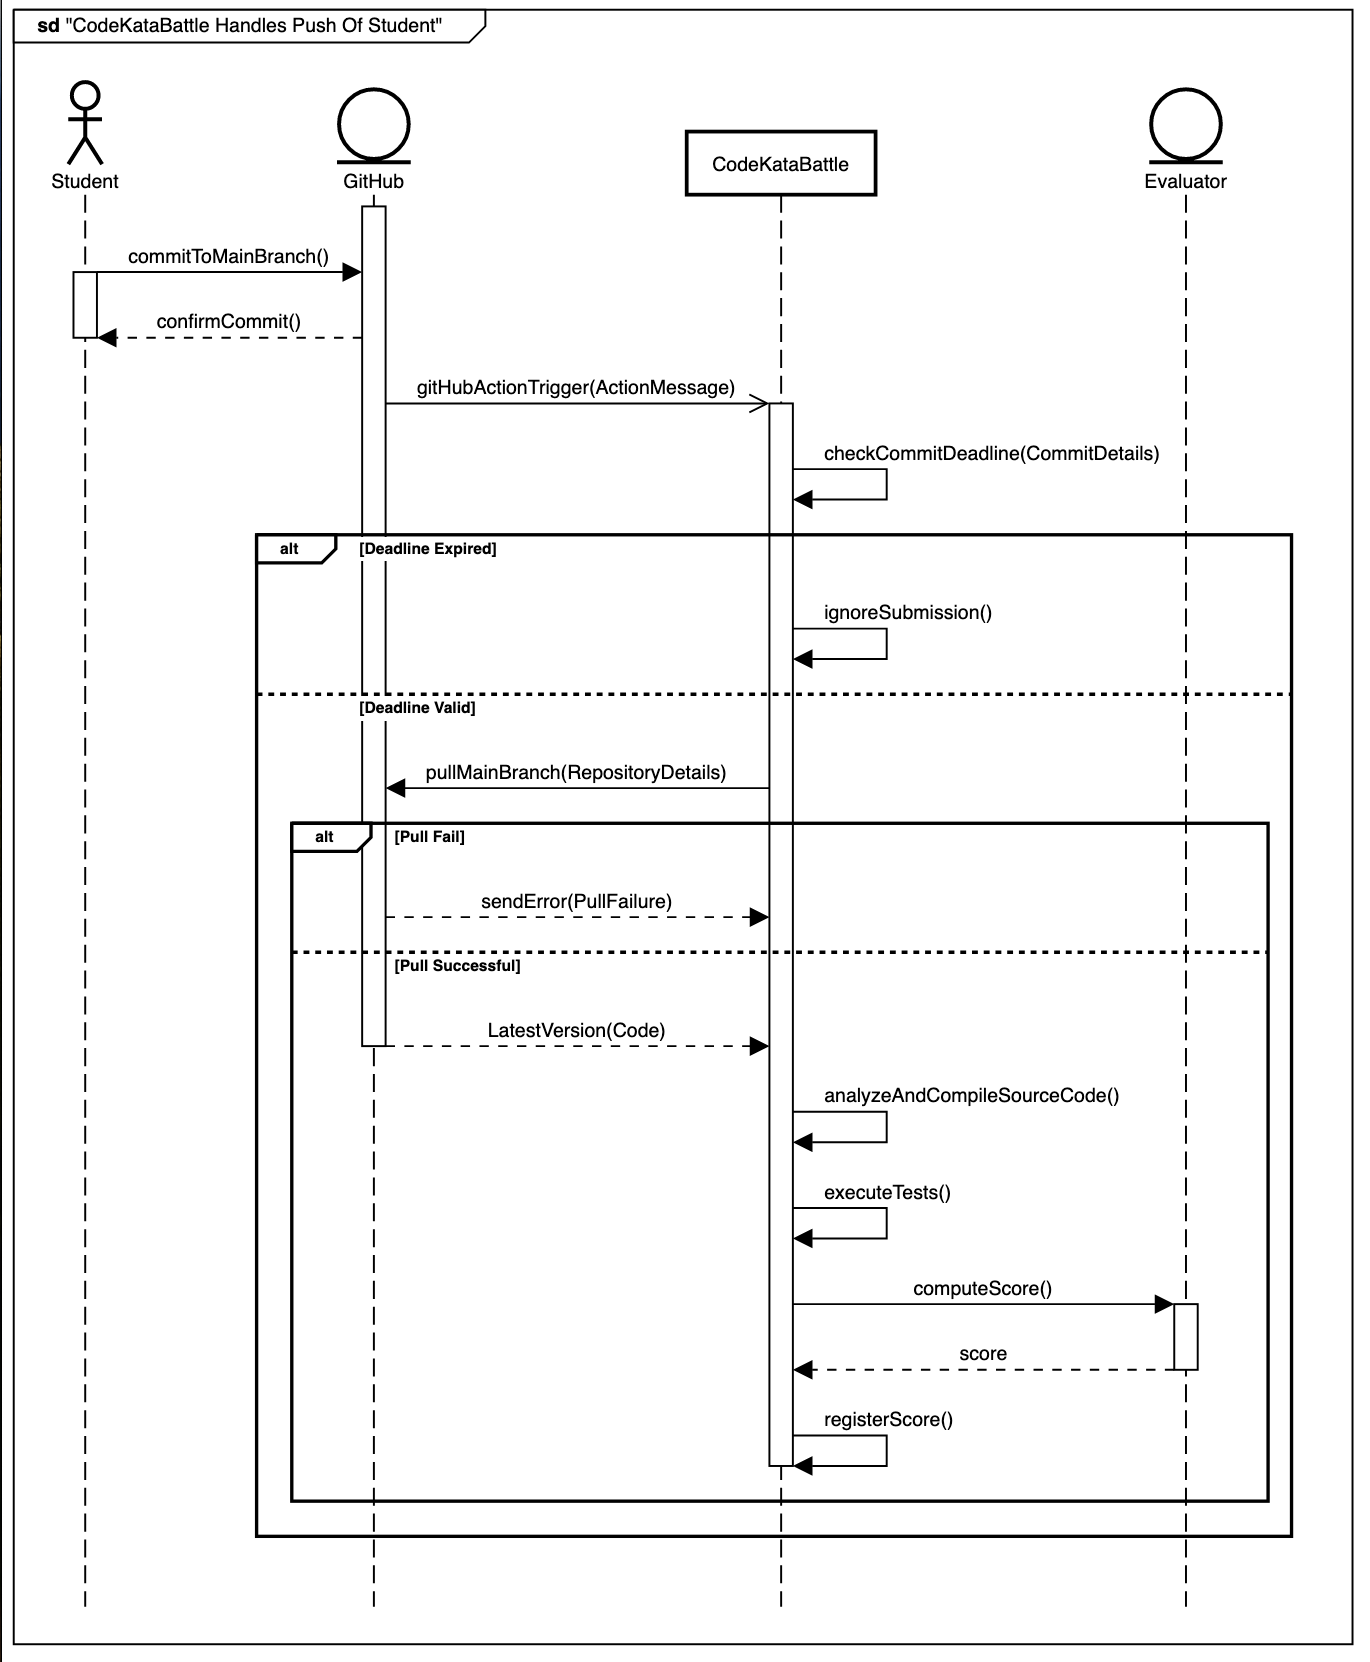
\includegraphics[scale = 0.45]{Images/SequenceDiagrams/StudentPushHandlerSeqDiagram.png}\\
\end{figure}

\newpage
\begin{xltabular}{\textwidth}{| l | X |}
\toprule
\multicolumn{2}{|c|}{BattleSubmissionDeadlineExpiration}\\
\toprule
Participating Actors & CodeKataBattle\\ [1ex]
\hline
Entry Condition & A Battle's submission deadline has reached its expiration point\\ [1ex]
\hline
Flow of Events & \begin{itemize}
		      \item 1. CodeKataBattle stops handling Students’ commits
		      \item 2. CodeKataBattle processes all enqueued commits
                \item 3. CodeKataBattle moves Battle to Consolidation Stage
                \end{itemize} \\ [1ex]
\hline
Exit Condition & The Battle scores and rankings are updated and it is in Consolidation Stage\\ [1ex]
\hline
Exceptions & None \\ [1ex]
\hline
\end{xltabular}
\begin{figure}[H]
\centering
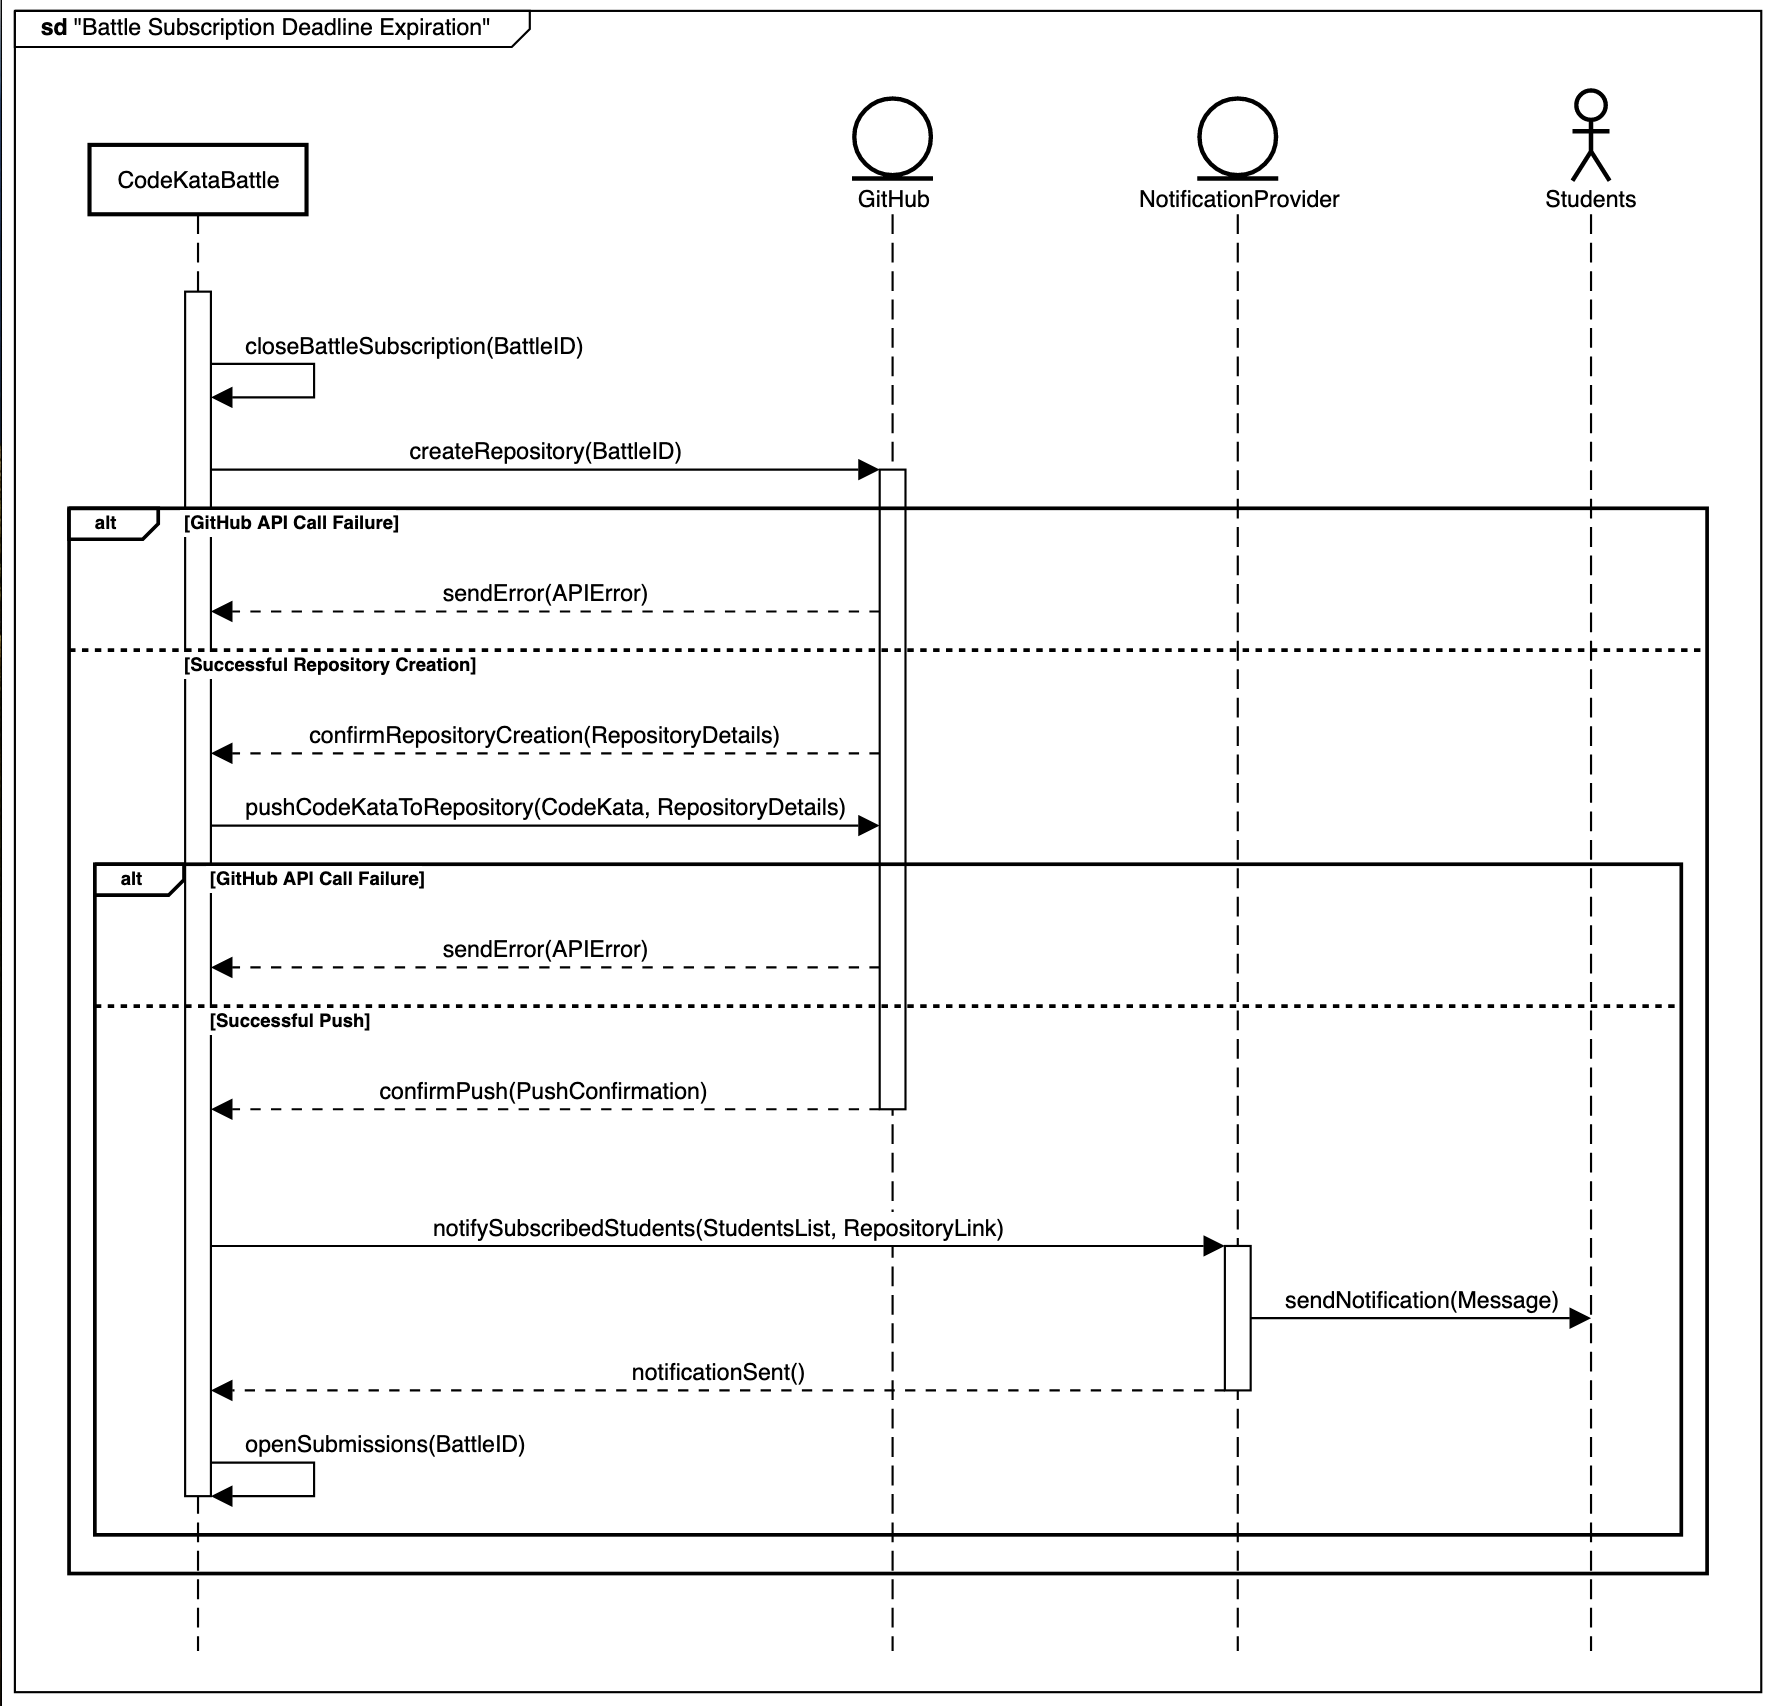
\includegraphics[scale = 0.45]{Images/SequenceDiagrams/BattleSubmDeadlineExpired.png}\\
\end{figure}
\newpage
\begin{xltabular}{\textwidth}{| l | X |}
\toprule
\multicolumn{2}{|c|}{EducatorEndsBattle}\\
\toprule
Participating Actors & Student, Educator, NotificationProvider, CodeKataBattle\\ [1ex]
\hline
Entry Condition & A Battle is in Consolidation Stage\\ [1ex]
\hline
Flow of Events & \begin{itemize}
		      \item 1. The Educator clicks on the “My Tournaments” button
		      \item 2. CodeKataBattle shows the list of the Tournaments that the Educator is allowed to manage
		      \item 3. The Educator clicks on a Tournament
		      \item 4. CodeKataBattle shows the Tournament’s details
		      \item 5. The Educator picks a Battle
                \item 6. The Educator eventually assigns manual further scores
                \item 7. The Educator clicks on "End Battle" button
                \item 8. CodeKataBattle ends the Battle
                \item 9. CodeKataBattle notifies through the NotificationProvider all the Students who participated in the Battle
                \end{itemize} \\ [1ex]
\hline
Exit Condition & The Battle has finished, the Tournament's personal scores of the Students are updated and the Students have been notified\\ [1ex]
\hline
Exceptions & None \\ [1ex]
\hline
\end{xltabular}
\begin{figure}[H]
\centering
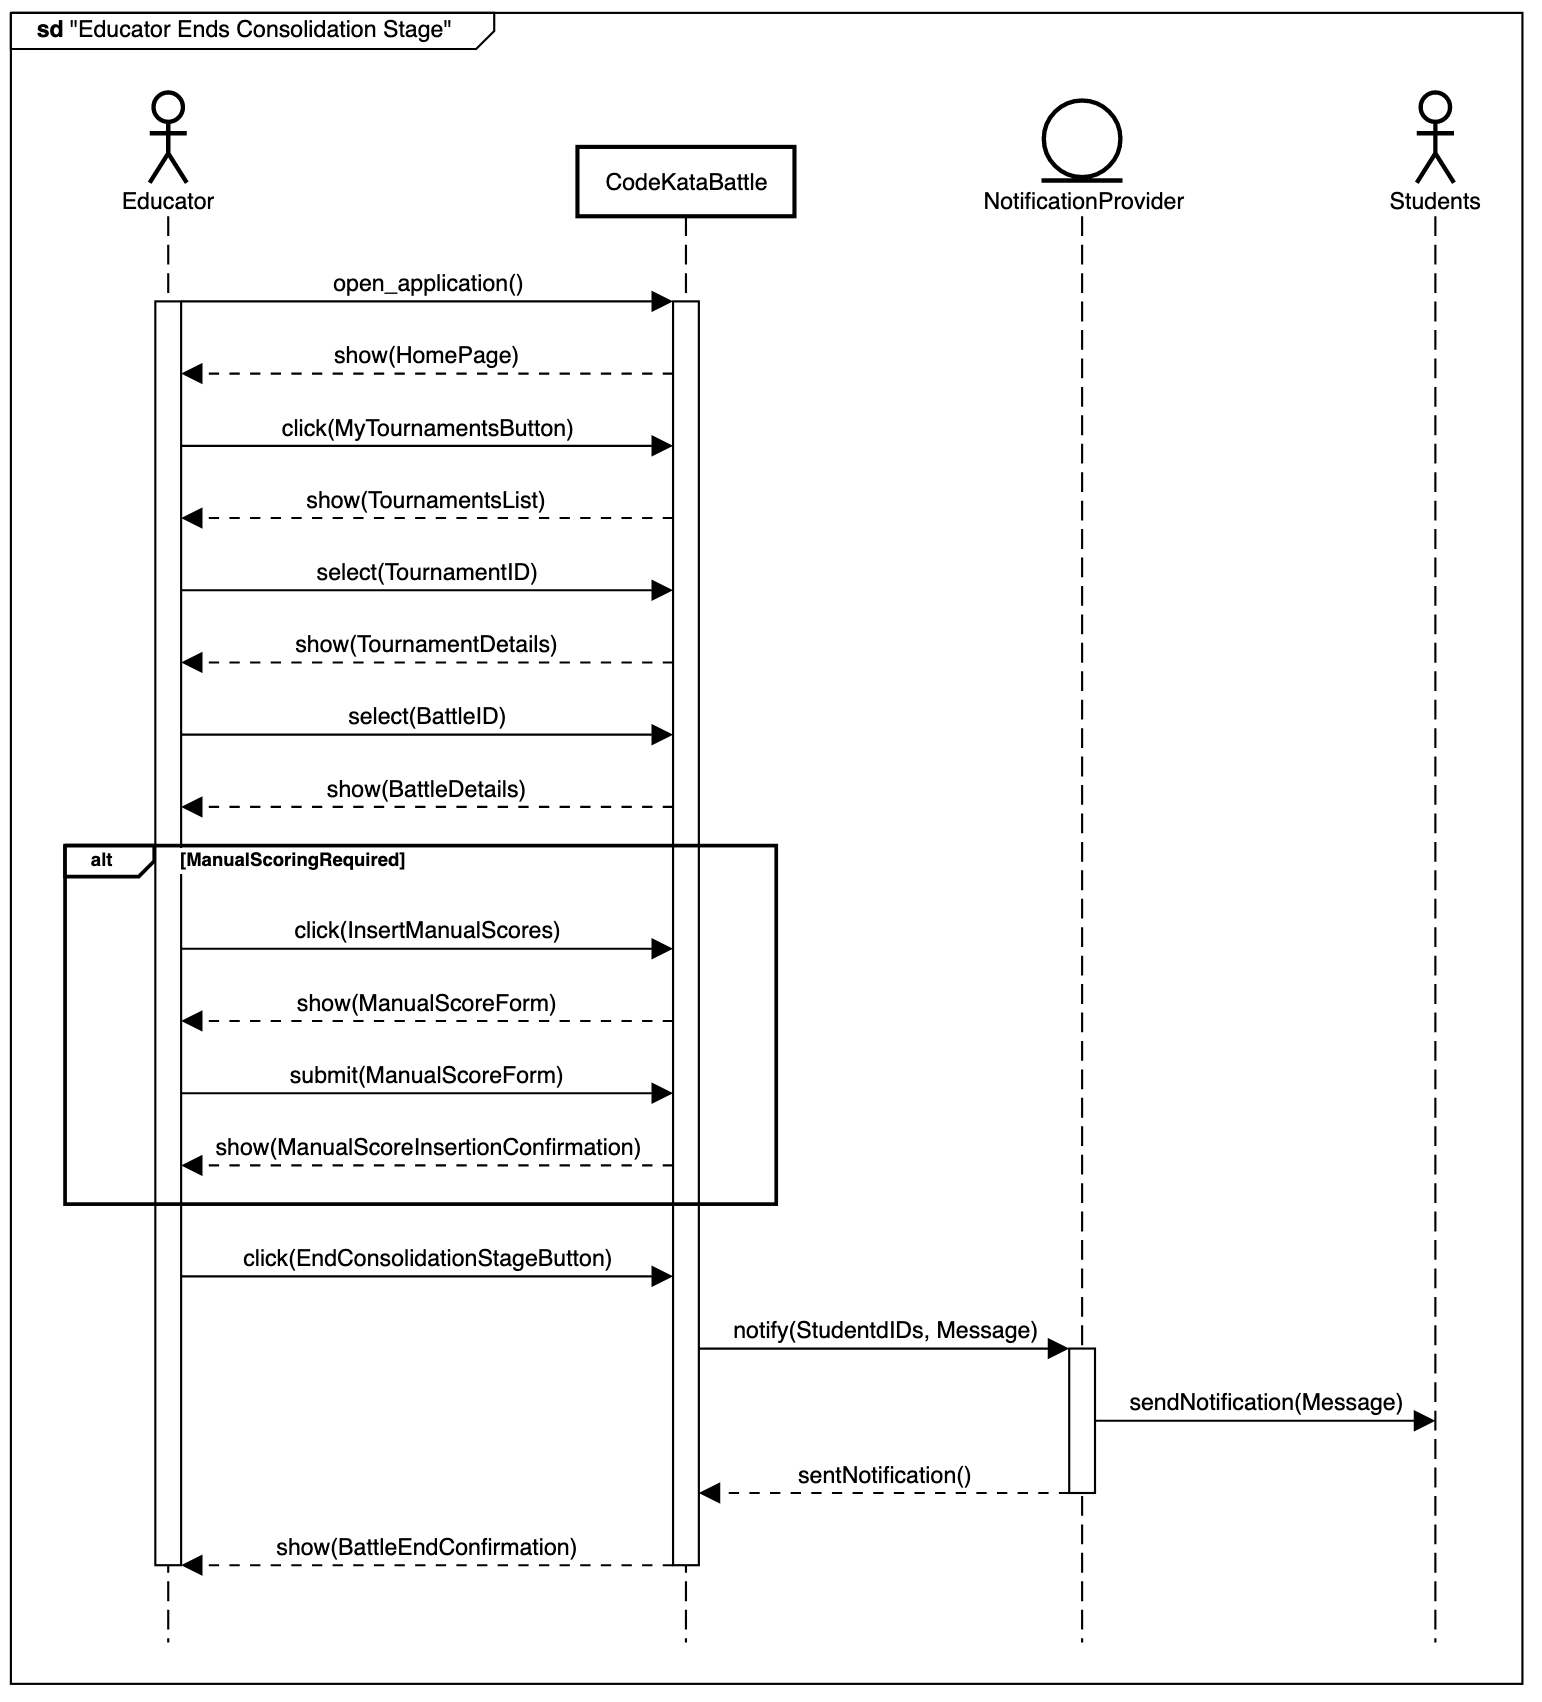
\includegraphics[scale = 0.45]{Images/SequenceDiagrams/EducatorEndsBattle.png}\\
\end{figure}
\newpage

\begin{xltabular}{\textwidth}{| l | X |}
\toprule
\multicolumn{2}{|c|}{EducatorClosesTournament}\\
\toprule
Participating Actors & Student, Educator, NotificationProvider, CodeKataBattle\\ [1ex]
\hline
Entry Condition & The Educator has the permission to manage the Tournament\\ [1ex]
\hline
Flow of Events & \begin{itemize}
		      \item 1. The Educator clicks on the “My Tournaments” button
		      \item 2. CodeKataBattle shows the list of the Tournaments that the Educator is allowed to manage
		      \item 3. The Educator clicks on a Tournament
		      \item 4. CodeKataBattle shows the Tournament’s details
		      \item 5. The Educator clicks on the “Close Tournament” button
                \item 6. CodeKataBattle closes the Tournament
                \item 7. CodeKataBattle computes the final Tournament ranking
                \item 8. CodeKataBattle eventually assigns Badges to the Students
                \item 9. CodeKataBattle notifies through the NotificationProvider all the Students who were subscribed to the Tournament
                \end{itemize} \\ [1ex]
\hline
Exit Condition & The Tournament is closed, all involved Students have been notified and Badges have been assigned \\ [1ex]
\hline
Exceptions & There is at least one Battle in the Tournament which is not finished \\ [1ex]
\hline
\end{xltabular}
\begin{figure}[H]
\centering
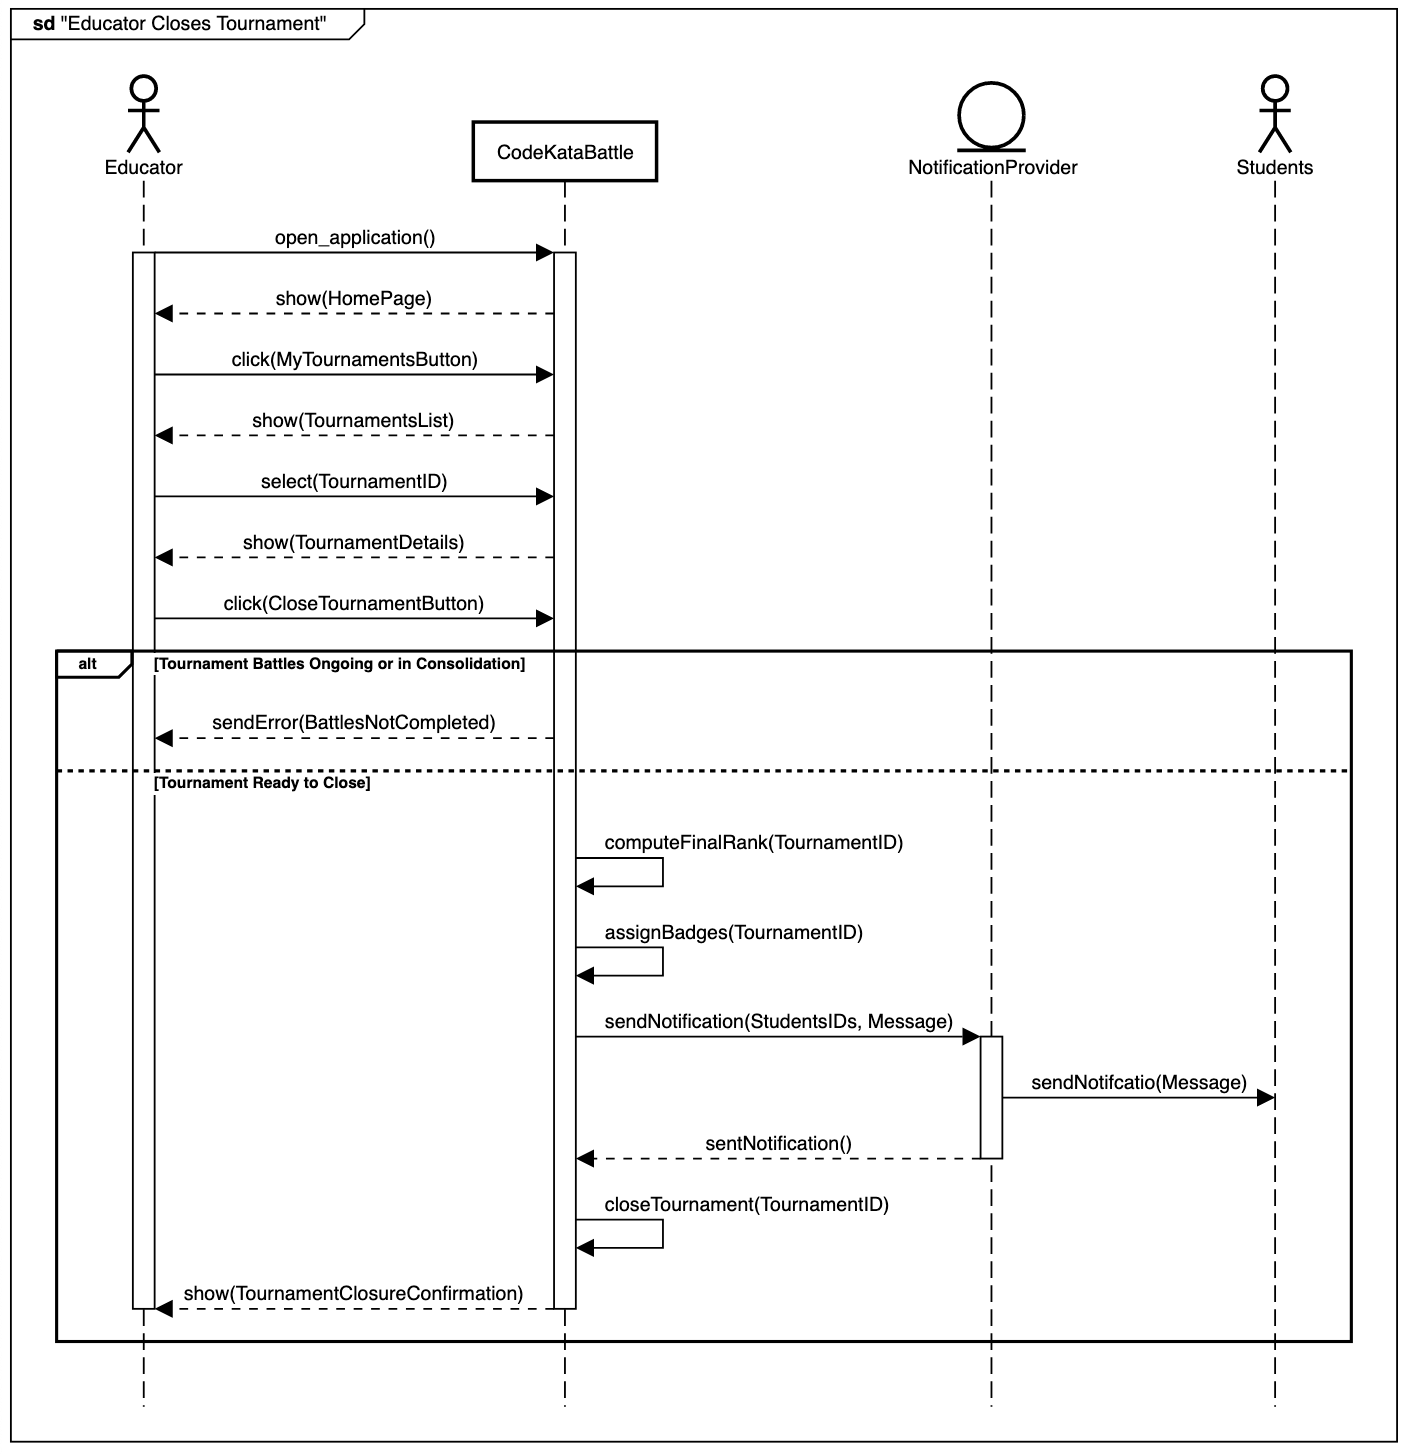
\includegraphics[scale = 0.45]{Images/SequenceDiagrams/EducatorClosesTournamentSeqDiagram.png}\\
\end{figure}
\newpage

\begin{xltabular}{\textwidth}{| l | X |}
\toprule
\multicolumn{2}{|c|}{UserVisualizesBattleRanking}\\
\toprule
Participating Actors & User, CodeKataBattle \\ [1ex]
\hline
Entry Condition & The Battle is started and the User is either an Educator who manages the Tournament of the Battle or a Students who is participating to the Battle \\ [1ex]
\hline
Flow of Events & \begin{itemize}
		      \item 1. The User clicks on the “My Tournaments” button
		      \item 2. CodeKataBattle shows the list of the Tournaments
		      \item 3. The Educator clicks on a Tournament
		      \item 4. CodeKataBattle shows the Tournament’s details
		      \item 5. The User clicks on a Battle
                \item 6. CodeKataBattle shows the Battle’s details
                \end{itemize} \\ [1ex]
\hline
Exit Condition & The User visualizes the current ranking for the Battle \\ [1ex]
\hline
Exceptions & None \\ [1ex]
\hline
\end{xltabular}
\begin{figure}[H]
\centering
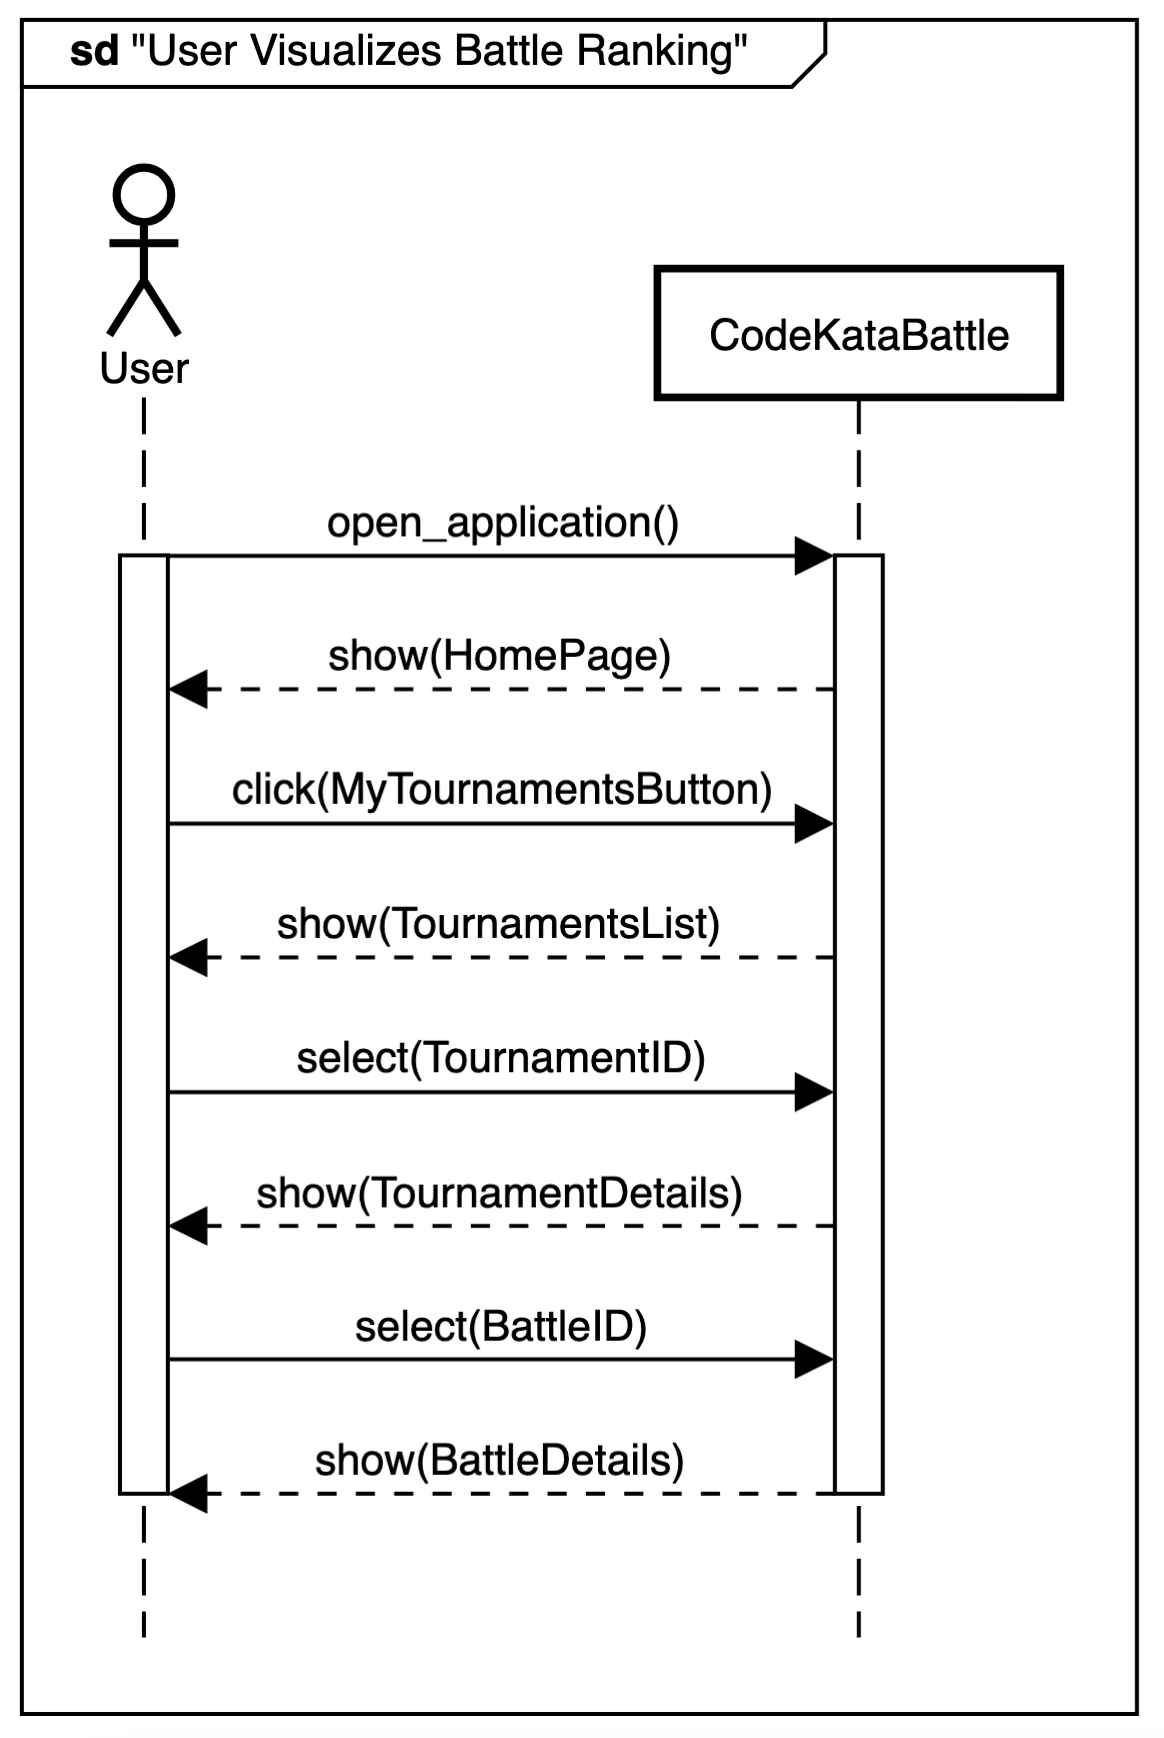
\includegraphics[scale = 0.45]{Images/SequenceDiagrams/UserVisualizesBattleRankingSeqDiagram.png}\\
\end{figure}

\newpage

\begin{xltabular}{\textwidth}{| l | X |}
\toprule
\multicolumn{2}{|c|}{UserVisualizesListTournaments}\\
\toprule
Participating Actors & User, CodeKataBattle \\ [1ex]
\hline
Entry Condition & User is logged in \\ [1ex]
\hline
Flow of Events & \begin{itemize}
		      \item 1. The User click on the “All Tournaments” button
		      \item 2. CodeKataBattle shows the list of the Tournaments
                \end{itemize} \\ [1ex]
\hline
Exit Condition & The User visualizes the list of Tournaments \\ [1ex]
\hline
Exceptions & None \\ [1ex]
\hline
\end{xltabular}
\begin{figure}[H]
\centering
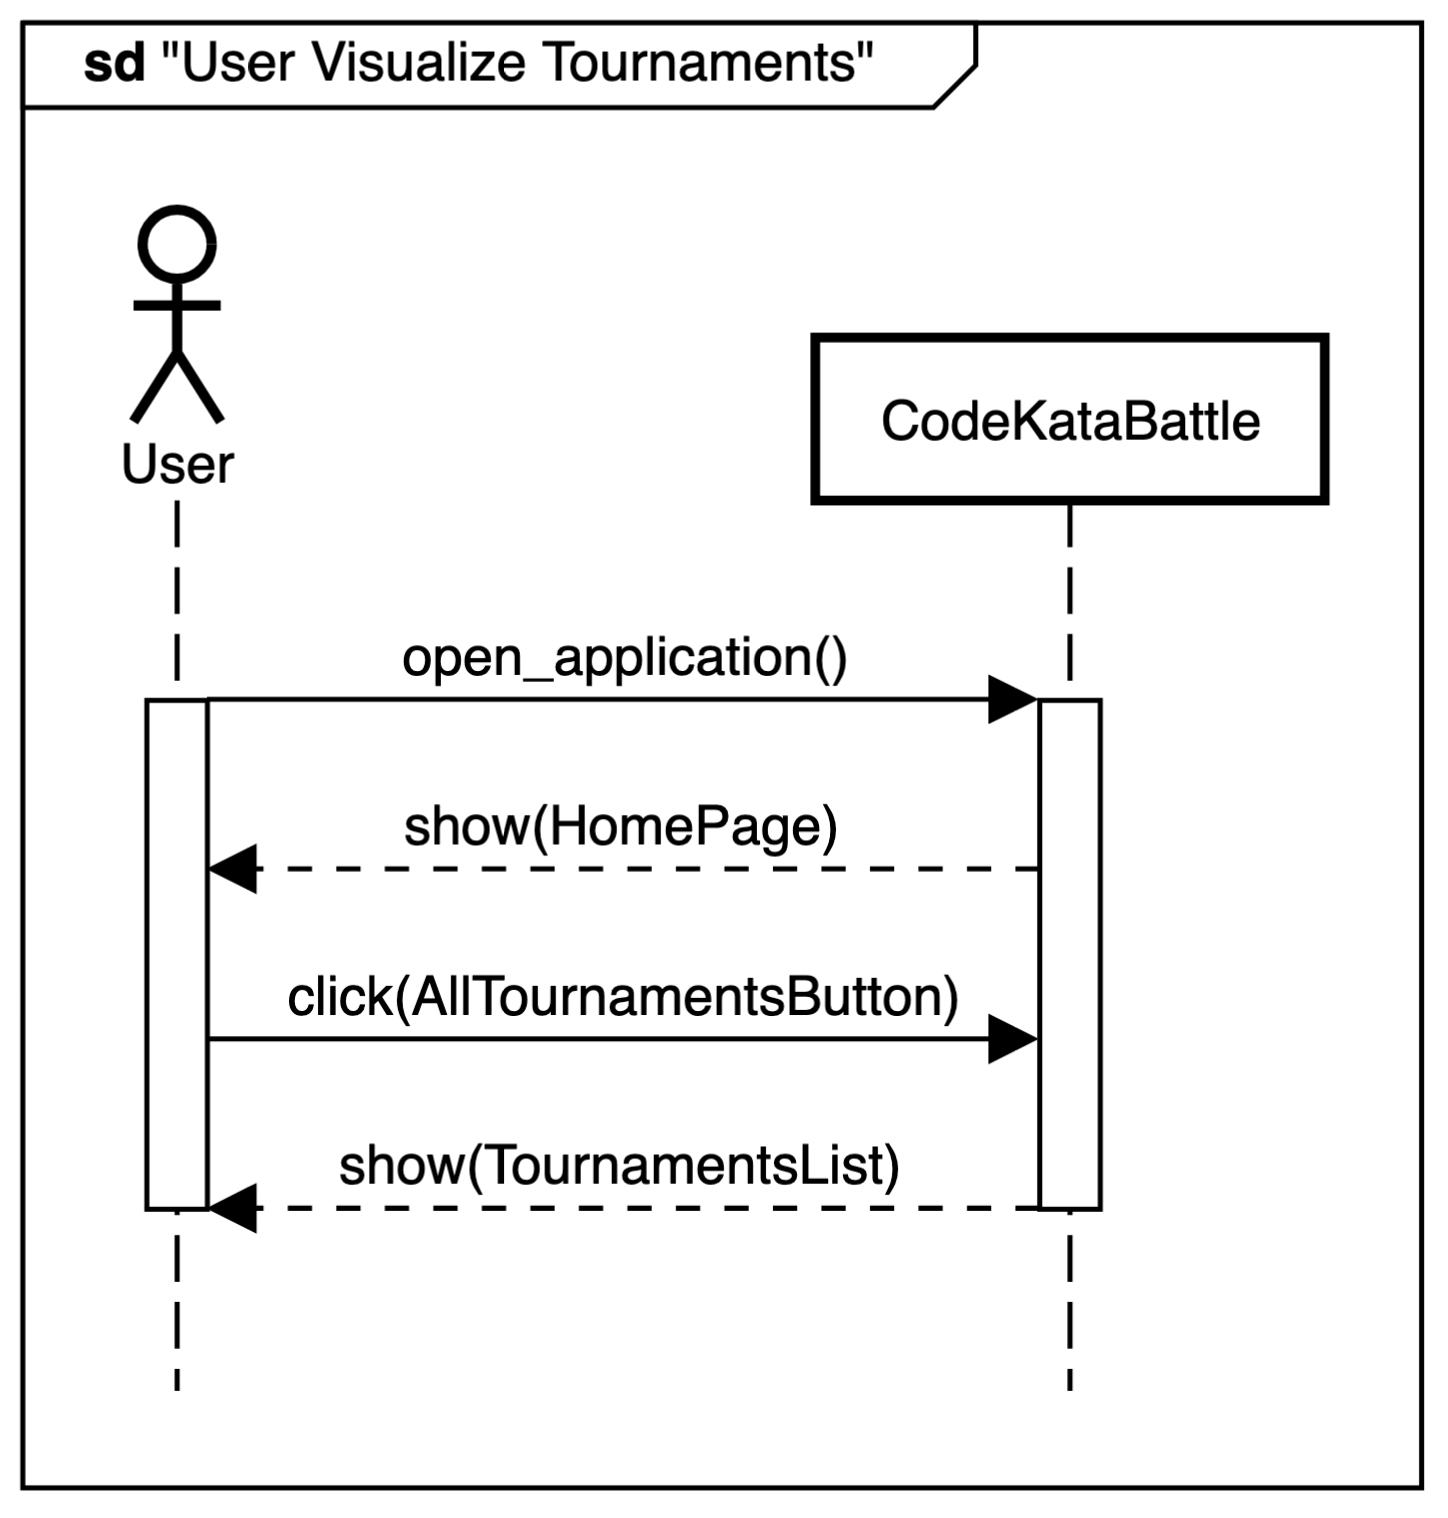
\includegraphics[scale = 0.45]{Images/SequenceDiagrams/UserVisualizesTournamentsSeqDiagram.png}\\
\end{figure}

\newpage

\begin{xltabular}{\textwidth}{| l | X |}
\toprule
\multicolumn{2}{|c|}{UserVisualizesTournamentRanking}\\
\toprule
Participating Actors & User, CodeKataBattle \\ [1ex]
\hline
Entry Condition & The Tournament has started and the User either an Educator who manages the Tournament or a Students who is subscribed to the Tournament \\ [1ex]
\hline
Flow of Events & \begin{itemize}
		      \item 1. The User click on the “My Tournaments” button
		      \item 2. CodeKataBattle shows the list of Tournaments
                \item 3. The User clicks on a Tournament
                \item 4. CodeKataBattle shows the Tournament’s details
                \end{itemize} \\ [1ex]
\hline
Exit Condition & The User visualizes the current ranking \\ [1ex]
\hline
Exceptions & None \\ [1ex]
\hline
\end{xltabular}
\begin{figure}[H]
    \centering
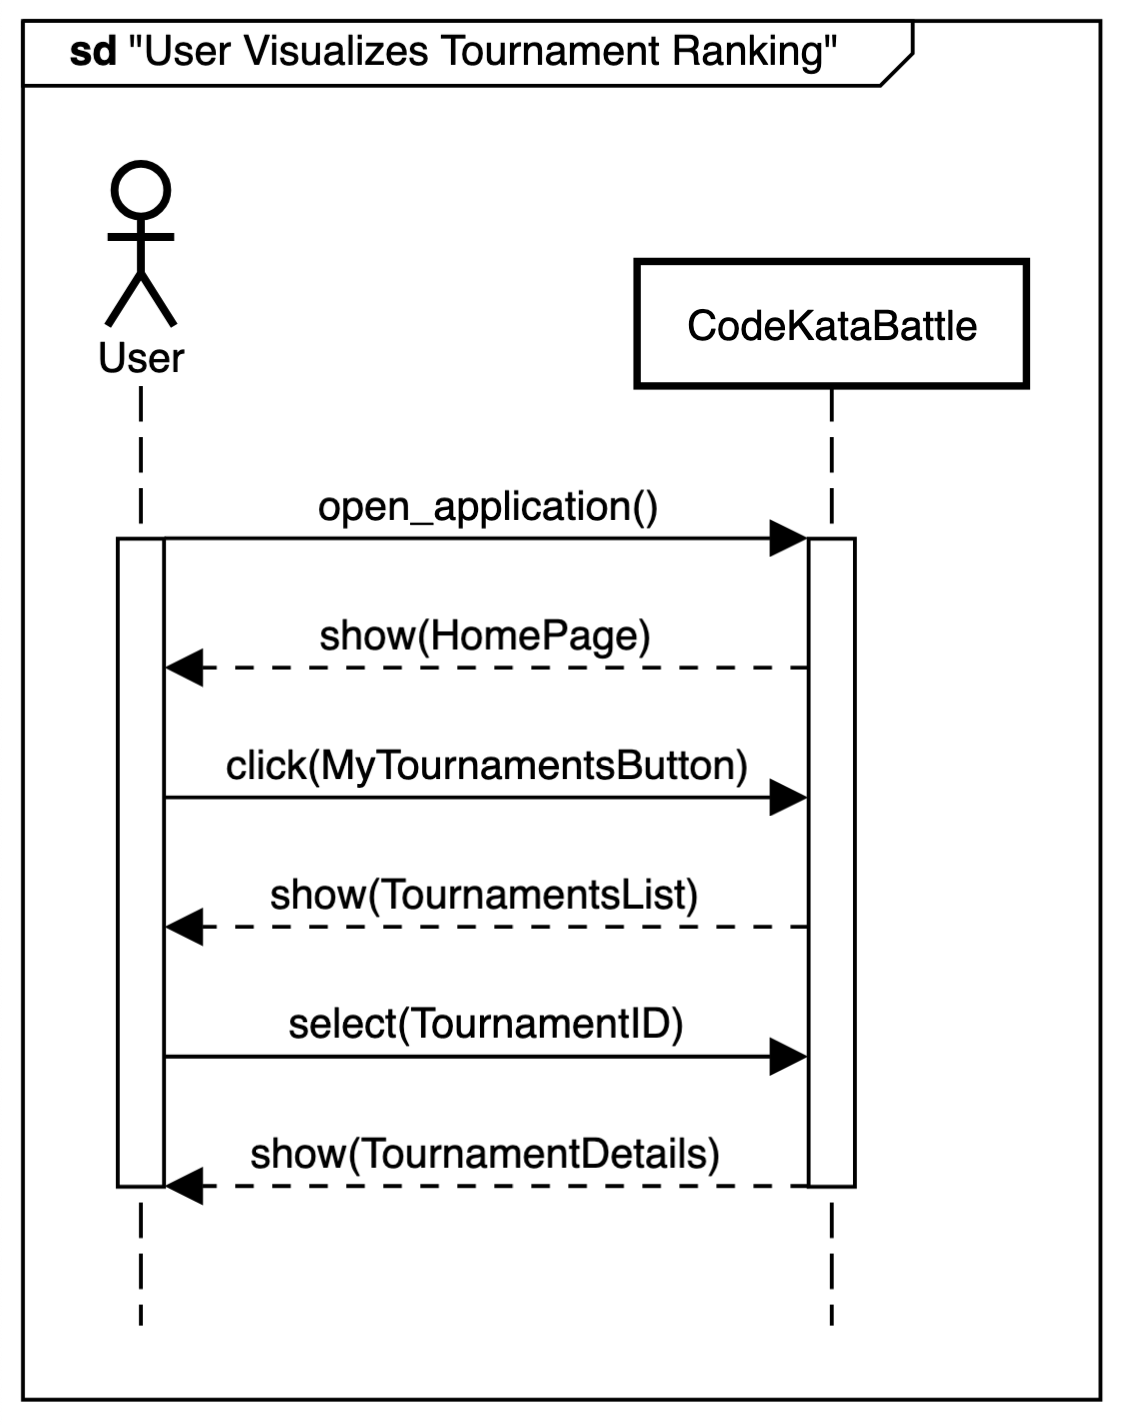
\includegraphics[scale = 0.45]{Images/SequenceDiagrams/UserVisualizesTournamentRankingSeqDiagram.png}\\

\end{figure}

\newpage

\begin{xltabular}{\textwidth}{| l | X |}
\toprule
\multicolumn{2}{|c|}{UserVisualizesStudentBadges}\\
\toprule
Participating Actors & User, CodeKataBattle \\ [1ex]
\hline
Entry Condition & True \\ [1ex]
\hline
Flow of Events & \begin{itemize}
		      \item 1. The User looks for the Student’s profile through the “Search” field
		      \item 2. CodeKataBattle shows the Students matching the query string
                \item 3. The User clicks on a Student
                \item 4. CodeKataBattle shows the Student’s profile details
                \end{itemize} \\ [1ex]
\hline
Exit Condition & The User visualizes the Student's Badges \\ [1ex]
\hline
Exceptions & The given query string is invalid \\ [1ex]
\hline
\end{xltabular}
\begin{figure}[H]
    \centering
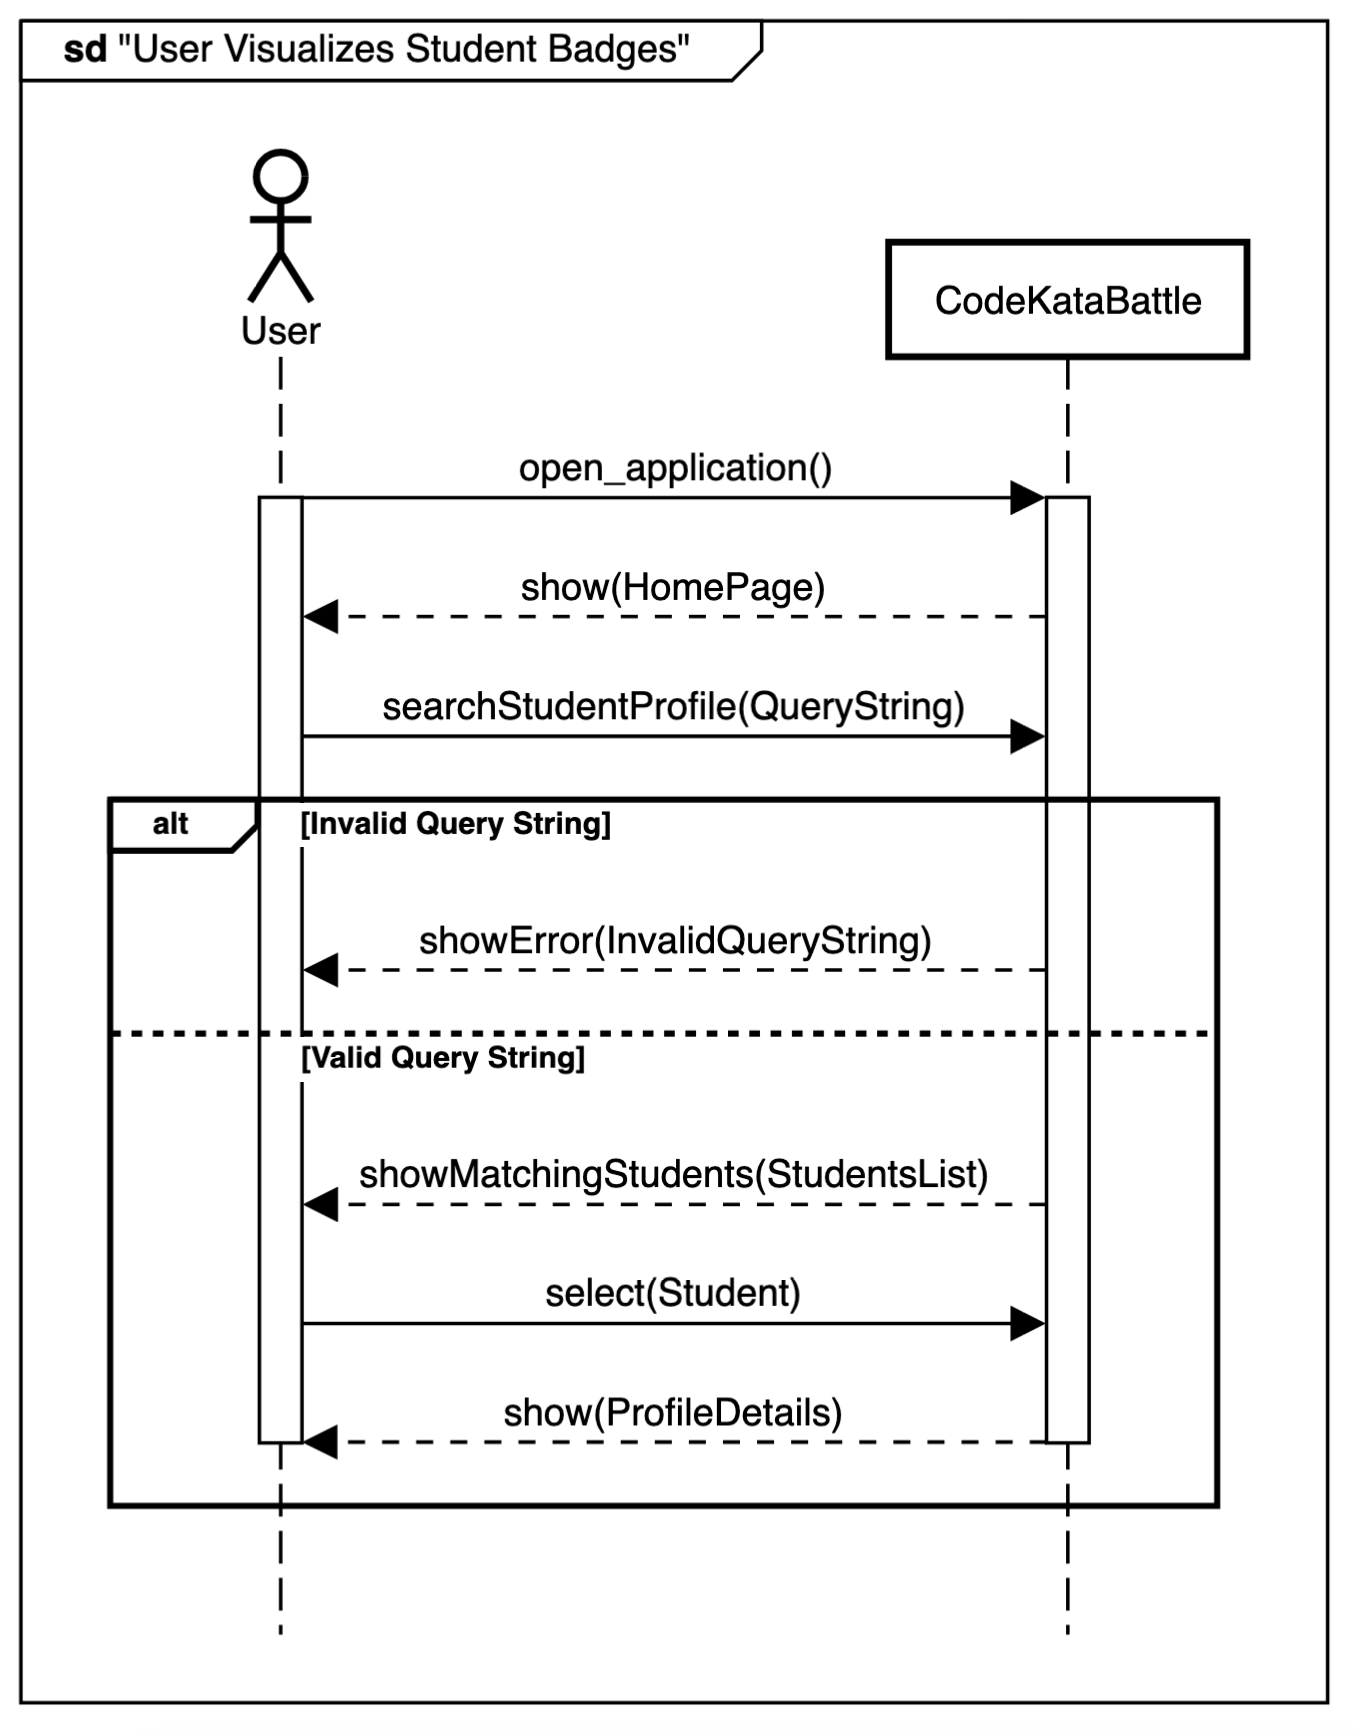
\includegraphics[scale = 0.45]{Images/SequenceDiagrams/UserVisualizesStudentBadgesSeqDiagram.png}\\
\end{figure}\

{\color{bluepoli}\rule{\linewidth}{0.1pt}}
\newpage
\subsection{Mapping}

{\color{bluepoli}\rule{\linewidth}{0.1pt}}
\\

\begin{xltabular}{\textwidth}{| l | X |}
\toprule
\multicolumn{2}{|c|}{G1}\\
\toprule
\textbf{G1} & \textbf{Allows registered Students who enrolled according to the right modalities to participate in a Tournament of Code Kata Battles and take part in its Battles.}\\ [1ex]
\hline
D1 & The User must have a working Internet connection.\\ [1ex]
\hline
D2 & The Students who participate to a Battle properly set up the GitHub Action for code submissions.\\ [1ex]
\hline
D3 & The Users always receive every notification which is sent by the system.\\ [1ex]
\hline
D4 & The availability of the external tools utilized for the code evaluation process is consistent.\\ [1ex]
\hline
D5 & The availability of GitHub Actions service is consistent.\\ [1ex]
\hline
R1 & The system must allow an unregistered Educator to sign up.\\ [1ex]
\hline
R2 & The system must allow an unregistered Student to sign up.\\ [1ex]
\hline
R3 & The system must allow a registered User to log in.\\ [1ex]
\hline
R4 & The system must allow registered Educators to start the creation process of a Tournament of Code Kata Battles.\\ [1ex]
\hline
R8 & The system must allow registered Educators to end the creation process of a Tournament that they started themselves.\\ [1ex]
\hline
R10 & The system must allow a registered Educator to create a Battle in a Tournament if and only if he is the creator of the Tournament or if he was granted the permission to by the latter.\\ [1ex]
\hline
R11 & The system must allow a registered Student to create a group for a Battle in a Tournament.\\ [1ex]
\hline
R12 & The system must allow a registered Student to accept an invitation to a group for a Battle in a Tournament.\\ [1ex]
\hline
R13 & The system must allow registered Students to see the list of ongoing Tournaments and join any of those if its subscription deadline is not expired yet.\\ [1ex]
\hline
R14 & The system must allow registered Students who are enrolled in a Battle to perform code submissions.\\ [1ex]
\hline
R17 & The system must set the Consolidation Stage of a Battle when its submission deadline expires.\\ [1ex]
\hline
R18 & The system must let Educators to end the Consolidation Stage of a Battle if and only if he is the creator of the Tournament or if he was granted the permission to by the latter.\\ [1ex]
\hline
R20 & The system must let Educators who are either the creator of the Tournament or who have been granted the permission to by the latter to close a Tournament if and only if there is no Battle such that either their subscription or submission deadline is not expired yet or such that they are still in the Consolidation Stage.\\ [1ex]
\hline
R23 & The system must notify every registered Student about the creation of a new Tournament.\\ [1ex]
\hline
R24 & The system must notify every registered Student about the creation of a new Battle within a Tournament they are enrolled in.\\ [1ex]
\hline
R25 & The system must notify every registered Student about the end of a Battle they are participating in.\\ [1ex]
\hline
R26 & The system must notify every registered Student about the end of a Tournament they are enrolled in.\\ [1ex]
\hline
\end{xltabular}

\begin{xltabular}{\textwidth}{| l | X |}
\toprule
\multicolumn{2}{|c|}{G2}\\
\toprule
\textbf{G2} & \textbf{Allows registered Educators to manage Tournaments for which they have been granted permission.}\\ [1ex]
\hline
D1 & The User must have a working Internet connection.\\ [1ex]
\hline
R1 & The system must allow an unregistered Educator to sign up.\\ [1ex]
\hline
R3 & The system must allow a registered User to log in.\\ [1ex]
\hline
R4 & The system must allow registered Educators to start the creation process of a Tournament of Code Kata Battles.\\ [1ex]
\hline
R7 & The system must allow registered Educators to grant other registered Educators the permission to manage the Tournament, during the Tournament creation process.\\ [1ex]
\hline
R8 & The system must allow registered Educators to end the creation process of a Tournament that they started themselves.\\ [1ex]
\hline
R10 & The system must allow a registered Educator to create a Battle in a Tournament if and only if he is the creator of the Tournament or if he was granted the permission to by the latter.\\ [1ex]
\hline
R18 & The system must let Educators to end the Consolidation Stage of a Battle if and only if he is the creator of the Tournament or if he was granted the permission to by the latter.\\ [1ex]
\hline
R20 & The system must let Educators who are either the creator of the Tournament or who have been granted the permission to by the latter to close a Tournament if and only if there is no Battle such that either their subscription or submission deadline is not expired yet or such that they are still in the Consolidation Stage.\\ [1ex]
\hline
\end{xltabular}

\begin{xltabular}{\textwidth}{| l | X |}
\toprule
\multicolumn{2}{|c|}{G3}\\
\toprule
\textbf{G3} & \textbf{Allows registered Students who participate in a Tournament of Code Kata Battles to be rewarded of different achievements.}\\ [1ex]
\hline
D1 & The User must have a working Internet connection.\\ [1ex]
\hline
D2 & The Students who participate to a Battle properly set up the GitHub Action for code submissions.\\ [1ex]
\hline
D3 & The Users always receive every notification which is sent by the system.\\ [1ex]
\hline
D4 & The availability of the external tools utilized for the code evaluation process is consistent.\\ [1ex]
\hline
D5 & The availability of GitHub Actions service is consistent.\\ [1ex]
\hline
R1 & The system must allow an unregistered Educator to sign up.\\ [1ex]
\hline
R2 & The system must allow an unregistered Student to sign up.\\ [1ex]
\hline
R3 & The system must allow a registered User to log in.\\ [1ex]
\hline
R4 & The system must allow registered Educators to start the creation process of a Tournament of Code Kata Battles.\\ [1ex]
\hline
R5 & The system must provide registered Educators of a list of Tournament-related statistics for the Badges definition, during the Tournament creation process.\\ [1ex]
\hline
R6 & The system must provide registered Educators of a specific language which lets them define the Badges, during the Tournament creation process.\\ [1ex]
\hline
R8 & The system must allow registered Educators to end the creation process of a Tournament that they started themselves.\\ [1ex]
\hline
R10 & The system must allow a registered Educator to create a Battle in a Tournament if and only if he is the creator of the Tournament or if he was granted the permission to by the latter.\\ [1ex]
\hline
R11 & The system must allow a registered Student to create a group for a Battle in a Tournament.\\ [1ex]
\hline
R12 & The system must allow a registered Student to accept an invitation to a group for a Battle in a Tournament.\\ [1ex]
\hline
R13 & The system must allow registered Students to see the list of ongoing Tournaments and join any of those if its subscription deadline is not expired yet.\\ [1ex]
\hline
R14 & The system must allow registered Students who are enrolled in a Battle to perform code submissions.\\ [1ex]
\hline
R17 & The system must set the Consolidation Stage of a Battle when its submission deadline expires.\\ [1ex]
\hline
R18 & The system must let Educators to end the Consolidation Stage of a Battle if and only if he is the creator of the Tournament or if he was granted the permission to by the latter.\\ [1ex]
\hline
R20 & The system must let Educators who are either the creator of the Tournament or who have been granted the permission to by the latter to close a Tournament if and only if there is no Battle such that either their subscription or submission deadline is not expired yet or such that they are still in the Consolidation Stage.\\ [1ex]
\hline
R21 & The system must assign an achievements’ Badge for a given Tournament to any Student who satisfied the conditions defined by the creator of the Tournament.\\ [1ex]
\hline
\end{xltabular}

\begin{xltabular}{\textwidth}{| l | X |}
\toprule
\multicolumn{2}{|c|}{G4}\\
\toprule
\textbf{G4} & \textbf{Allows registered Users to visualize information for which they have granted permission.}\\ [1ex]
\hline
D1 & The User must have a working Internet connection.\\ [1ex]
\hline
R1 & The system must allow an unregistered Educator to sign up.\\ [1ex]
\hline
R2 & The system must allow an unregistered Student to sign up.\\ [1ex]
\hline
R3 & The system must allow a registered User to log in.\\ [1ex]
\hline
R4 & The system must allow registered Educators to start the creation process of a Tournament of Code Kata Battles.\\ [1ex]
\hline
\hline
R8 & The system must allow registered Educators to end the creation process of a Tournament that they started themselves.\\ [1ex]
\hline
R10 & The system must allow a registered Educator to create a Battle in a Tournament if and only if he is the creator of the Tournament or if he was granted the permission to by the latter.\\ [1ex]
\hline
R11 & The system must allow a registered Student to create a group for a Battle in a Tournament.\\ [1ex]
\hline
R12 & The system must allow a registered Student to accept an invitation to a group for a Battle in a Tournament.\\ [1ex]
\hline
R13 & The system must allow registered Students to see the list of ongoing Tournaments and join any of those if its subscription deadline is not expired yet.\\ [1ex]
\hline
R16 & The system must update the Battle ranking when a valid code submission is performed.\\ [1ex]
\hline
R17 & The system must set the Consolidation Stage of a Battle when its submission deadline expires.\\ [1ex]
\hline
R18 & The system must let Educators to end the Consolidation Stage of a Battle if and only if he is the creator of the Tournament or if he was granted the permission to by the latter.\\ [1ex]
\hline
R19 & The system must update Tournament ranking when a Battle exits the Consolidation Stage.\\ [1ex]
\hline
R20 & The system must let Educators who are either the creator of the Tournament or who have been granted the permission to by the latter to close a Tournament if and only if there is no Battle such that either their subscription or submission deadline is not expired yet or such that they are still in the Consolidation Stage.\\ [1ex]
\hline
R21 & The system must assign an achievements’ Badge for a given Tournament to any Student who satisfied the conditions defined by the creator of the Tournament.\\ [1ex]
\hline
R22 & The system must allow every User to see the Badges which were ever obtained by a given Student.\\ [1ex]
\hline
\end{xltabular}

\begin{xltabular}{\textwidth}{| l | X |}
\toprule
\multicolumn{2}{|c|}{G5}\\
\toprule
\textbf{G5} & \textbf{Automates code evaluation process using GitHub Actions and other external tools.}\\ [1ex]
\hline
D2 & The Students who participate to a Battle properly set up the GitHub Action for code submissions.\\ [1ex]
\hline
D4 & The availability of the external tools utilized for the code evaluation process is consistent.\\ [1ex]
\hline
D5 & The availability of GitHub Actions service is consistent.\\ [1ex]
\hline
R1 & The system must allow an unregistered Educator to sign up.\\ [1ex]
\hline
R2 & The system must allow an unregistered Student to sign up.\\ [1ex]
\hline
R3 & The system must allow a registered User to log in.\\ [1ex]
\hline
R4 & The system must allow registered Educators to start the creation process of a Tournament of Code Kata Battles.\\ [1ex]
\hline
\hline
R8 & The system must allow registered Educators to end the creation process of a Tournament that they started themselves.\\ [1ex]
\hline
R10 & The system must allow a registered Educator to create a Battle in a Tournament if and only if he is the creator of the Tournament or if he was granted the permission to by the latter.\\ [1ex]
\hline
R11 & The system must allow a registered Student to create a group for a Battle in a Tournament.\\ [1ex]
\hline
R12 & The system must allow a registered Student to accept an invitation to a group for a Battle in a Tournament.\\ [1ex]
\hline
R13 & The system must allow registered Students to see the list of ongoing Tournaments and join any of those if its subscription deadline is not expired yet.\\ [1ex]
\hline
R14 & The system must allow registered Students who are enrolled in a Battle to perform code submissions.\\ [1ex]
\hline
R15 & The system must be provided of proper APIs to let registered Students perform code submissions through GitHub Actions.\\ [1ex]
\hline
\end{xltabular}

{\color{bluepoli}\rule{\linewidth}{0.1pt}}

\section{Performance Requirements}

Due to the non-critical nature of the system, too strict performance requirements are not needed. 
However, in order to offer the best possible User experience, the system should provide:

\begin{itemize}
\item The system should let Educators create a Tournament within 2 seconds.
\item The system should let Educators create a Battle within 2 seconds.
\item The system should let Students join a Tournament within 2 seconds
\item The system should let Students join a Battle within 2 seconds
\item The system should receive a code submission by a Student within 5 seconds
\item The system should evaluate code submissions within 180 seconds
\item The system should update the Battle ranking within 2 seconds
\item The system should update the Tournament ranking within 2 seconds
\item The system should let Educators end the Consolidation Stage of a Battle within 5 seconds.
\item The system should let Educators end a Tournament within 5 seconds.
\item The system should let new Badges be available in the Students profiles within 2 seconds\\
\end{itemize}
{\color{bluepoli}\rule{\linewidth}{0.1pt}}

\section{Design Constraints}

In this section some information about the design constraint is provided.

{\color{bluepoli}\rule{\linewidth}{0.1pt}}

\subsection{Standards compliance}

Specifications described in this document must be respected by the system. The source code of the application must be commented on and documented adequately.\\
The system should respect the guidelines described by the GDPR.

{\color{bluepoli}\rule{\linewidth}{0.1pt}}

\subsection{Hardware limitations}

The system requires any device and a stable internet connection.

{\color{bluepoli}\rule{\linewidth}{0.1pt}}

\section{Software System Attributes}

In this section typically, the non-functional requirements and quality attributes of the system which should be provided are discussed. 

\subsection{Reliability and Availability}

{\color{bluepoli}\rule{\linewidth}{0.1pt}}

The system should offer its functionalities with an availability equal to 99.5\%, or more. In other words, the system must be inaccessible for less than two days every year. To achieve this goal, the system should provide a high redundancy for the most critical components.\\
Furthermore, in order to guarantee better reliability performances, all the scheduled maintenance actions on the system should be done during the night.\\

{\color{bluepoli}\rule{\linewidth}{0.1pt}}

\subsection{Security}

{\color{bluepoli}\rule{\linewidth}{0.1pt}}

The connection between the application and the server must be safe. To keep a good level of security, the system should use the Transport Layer Security protocol. For this purpose, it is needed an SSL/TSL certificate.

{\color{bluepoli}\rule{\linewidth}{0.1pt}}

\subsection{Maintainability}

{\color{bluepoli}\rule{\linewidth}{0.1pt}}

The source code must be commented on as well as possible and the correlated documentation must be kept updated during the whole life cycle of the system.\\
Modularity and low coupling between components must be a focus during the designing and developing phases.\\

{\color{bluepoli}\rule{\linewidth}{0.1pt}}

% FOURTH CHAPTER
% --------------------------------------------------------------------------
\chapter{Formal analysis using alloy}

\section{Objectives of the analysis}

In this section, a presentation of the formal modelling activity that has been done using the Alloy formal notation. The main goal of this activity is to formally describe the domain and properties of the system to be.\\
In particular, the main objective of this activity is to model and formally represent Educators, Students, Tournaments, Battles and Badges, as well as the main constraints which regard such entities.\\
In order to ensure straightforward comprehension of the following, each constraint and entity will be annotated in natural language, along with any predicates and assertions which have been verified.\\

{\color{bluepoli}\rule{\linewidth}{0.1pt}}

\section{Alloy Code}

// -------------- Definition of auxiliar entities -------------- //\\

// Defined in order to model the deadlines

sig Time \{\\
timestamp: Int\\
\}\{\\
timestamp >= 0\\
\}\\

// Defined in order to model any flag, such as whether a Battle is in the Consolidation Stage
abstract sig Boolean \{\}
one sig True extends Boolean \{\}
one sig False extends Boolean \{\}\\

// -------------- Definition of game components -------------- //\\

// Defined in order to model the score of a team in a Battle and the score of a Student in a Tournament
sig Score \{\\
value: Int\\
\}\{\\
value >= 0\\
\}\\

// Defined in order to model the rank of a team in a Battle and the rank of a Student in a Tournament
sig Rank \{\\
value: Int\\
\}\{\\
value >= 1\\
\}\\

// Defined in order to model the Tournament
sig Tournament \{\\
managers: some Educator,\\
subscription\_deadline: one Time,\\
battles: set Battle,\\
scores: Student -> one Score,\\
ranks: Student -> one Rank,
badges: set Badge,\\
achievements: Student -> set BadgeRule\\
\}\\

// Defined in order to model the Battle (unnecessary to model the programming language)
sig Battle \{\\
tournament: one Tournament,\\
teams: Student -> some Student,\\
scores: Student -> one Score,\\
ranks: Student -> one Rank,\\
subscription\_deadline: one Time,\\
submission\_deadline: one Time,\\
consolidation\_stage: one Boolean\\
\}\\

// Defined in order to model the Badge (unnecessary to model the title)
sig BadgeRule \{\\
\}
sig Badge \{\\
rule: one BadgeRule\\
\}\\

// -------------- Definition of actors -------------- //\\

// Defined in order to model the nature of Student and Educator as Users
abstract sig User \{\}\\

// Defined in order to model the Student
sig Student extends User \{\\
badges: set Badge\\
\}\\

// Defined in order to model the Educator
sig Educator extends User\{\\
\}\\

//  -------------- Facts -------------- //\\

// Tournaments: A Student must both have a score and a rank, if a Student has higher score than another Student than it has a lower rank (e.g. 1st is lower than 2nd), only achievements of Badges which relate to existing Badges for the Tournament are stored, a Student has one only score, a Student has one only rank
fact TournamentFact \{\\

    all t1: Tournament | all s: Student | some sc: Score | some r: Rank | ( sc in s.(t1.scores) ) => ( r in s.(t1.ranks) ) and ( r in s.(t1.ranks) => sc in s.(t1.scores) )\\
    all t2: Tournament | all s1, s2: Student | ( ( s1.(t2.ranks).value < s2.(t2.ranks).value ) <=> ( s1.(t2.scores).value > s2.(t2.scores).value ) )\\
    all t3: Tournament | all s3: Student | all b: Badge | ( b.rule in s3.(t3.achievements) ) => ( b in t3.badges )\\
    all t4: Tournament | all disj sc1, sc2: Score | some s: Student | ( sc1 in s.(t4.scores) ) => not ( sc2 in s.(t4.scores) )\\
    all t5: Tournament | all disj r1, r2: Rank | some s: Student | ( r1 in s.(t5.ranks) ) => not ( r2 in s.(t5.ranks) )\\
\}\\

// Battles: The subscription deadline must expire before the submission deadline, teams relationships are symmetrical, teams relationships are reflexive, if a Student s1 is in team with a Student s2 and not with a Student s3 then s2 is not in team with s3, Students in the same team have same score and rank, a Student has one only score, a Student has one only rank\\

fact BattleFact \{\\
    all b: Battle | b.subscription\_deadline.timestamp < b.submission\_deadline.timestamp\\
    all b1: Battle | all s1, s2: Student | s2 in s1.(b1.teams) <=> s1 in s2.(b1.teams)\\
    all b2: Battle | all s: Student | s in s.(b2.teams)\\
    all b3: Battle | all s3, s4, s5: Student | ( ( s4 in s3.(b3.teams) )  and ( not ( s5 in s3.(b3.teams) ) ) ) => ( not (s4 in s5.(b3.teams) ) )\\
    all b4: Battle | all s6, s7: Student | s7 in s6.(b4.teams) => ( ( s6.(b4.scores).value = s7.(b4.scores).value ) and ( s6.(b4.ranks).value = s7.(b4.scores).value ) )\\
    all b5: Battle | all disj sc1, sc2: Score | some s8: Student | ( sc1 in s8.(b5.scores) ) => ( not ( sc2 in s8.(b5.scores) ) )\\
    all b6: Battle | all disj r1, r2: Rank | some s9: Student | ( r1 in s9.(b6.ranks) ) => ( not ( r2 in s9.(b6.ranks) ) )\\
\}\\

// A Student must have obtained the Badges in some Tournament\\

fact StudentObtainedBadges \{\\
one t: Tournament | all s: Student, b: Badge | b in s.badges => b.rule in s.(t.achievements)\\
\}\\

// -------------- Predicates and assertions -------------- //\\

//  1. A basic example\\

pred show \{\\
some b: Battle | some t: Tournament | b in t.battles\\
\}\\
run show\\

\begin{figure}[H]
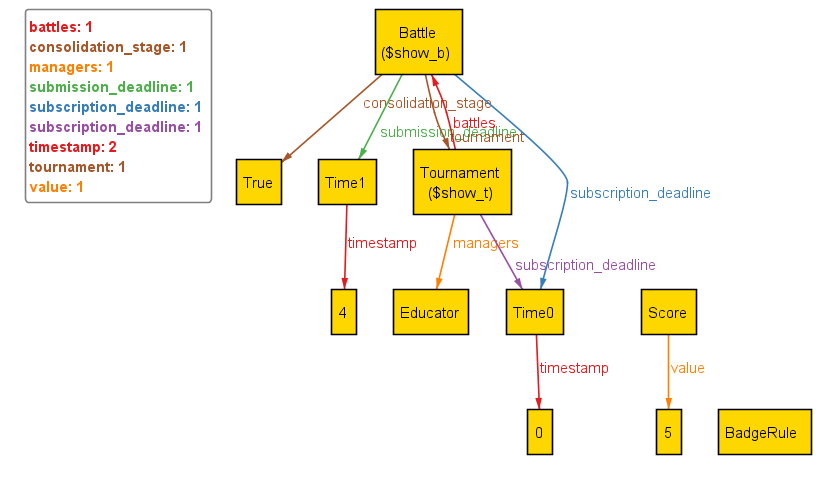
\includegraphics[scale = 0.7]{Images/Alloy/1Model.png}\\
\centering
\end{figure}
\begin{figure}[H]
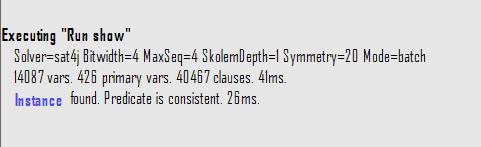
\includegraphics[scale = 0.7]{Images/Alloy/1Outcome.png}\\
\centering
\end{figure}

//  2. An example to show that a higher position in the ranking corresponds to a lower score\\

pred RankingExample \{\\
some disj b1, b2: Battle | some t: Tournament | b1 in t.battles and b2 in t.battles\\
some disj s3, s4: Student | some b3: Battle | ( not ( s3 in s4.(b3.teams) ) ) and ( s3.(b3.ranks).value != s4.(b3.ranks).value )\\
some r1, r2: Rank | r1.value = 1 and r2.value = 2\\
some sc1, sc2: Score | ( sc1. value = 5 ) and ( sc2.value = 6 )\\
\}\\
run RankingExample\\

\begin{figure}[H]
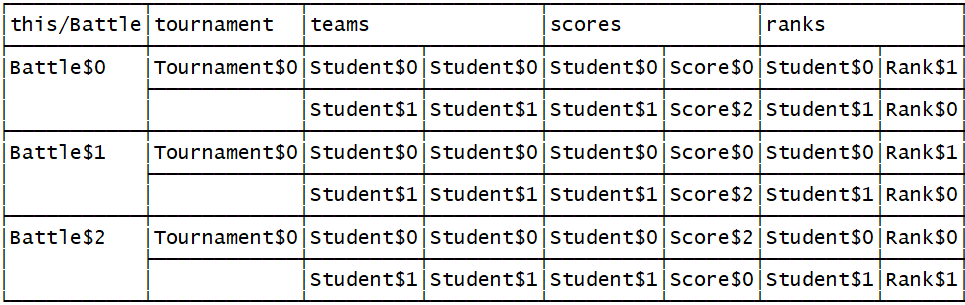
\includegraphics[scale = 0.7]{Images/Alloy/2Table1.png}\\
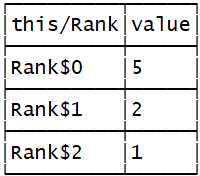
\includegraphics[scale = 0.7]{Images/Alloy/2Table2.png}\\
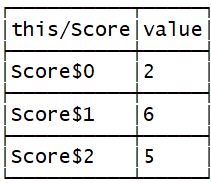
\includegraphics[scale = 0.7]{Images/Alloy/2Table3.png}\\
\centering
\end{figure}
\begin{figure}[H]
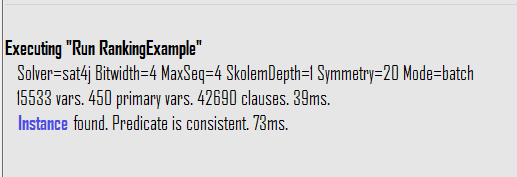
\includegraphics[scale = 0.7]{Images/Alloy/2Outcome.png}\\
\centering
\end{figure}

//  3. Ensuring that Badges obtained by Students must be existed in some Tournaments (in this model, Tournament can both represent both a running one or a finished one)\\
assert ExistingBadges \{\\
all b: Badge | all s: Student | some t: Tournament | ( b in s.badges ) => ( b in t.badges)\\
\}\\
check ExistingBadges\\

\begin{figure}[H]
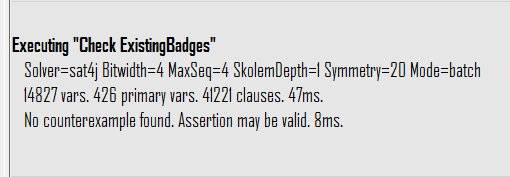
\includegraphics[scale = 0.7]{Images/Alloy/3Outcome.png}\\
\centering
\end{figure}

{\color{bluepoli}\rule{\linewidth}{0.1pt}}


% FIFTH CHAPTER
% --------------------------------------------------------------------------
\chapter{Effort spent}
\section{Effort spent per unit}

This section shows the amount of time that each member has spent to produce the document. Please notice that each unit is the result of coordinated work among all the members.

\begin{table}[h]
\centering
\begin{tabularx}{\textwidth}{| X | X | X |}
\hline
\textbf{UNIT} & \textbf{MEMBERS} & \textbf{HOURS} \\ [1ex]
\hline
SetUp & Puglisi & 1h \\ [1ex]
\hline
Scenarios & Piccinato & 3h \\ [1ex]
\hline
Use Cases & Piazzalunga, Piccinato & 8h \\ [1ex]
\hline
Phenomena & Puglisi, Piccinato & 5h \\ [1ex]
\hline
Goals & Puglisi, Piccinato & 2h \\ [1ex]
\hline
Domain Assumptions & Piccinato, Puglisi & 1h \\ [1ex]
\hline
Requirements & Piccinato, Puglisi & 7h \\ [1ex]
\hline
Mapping & Piccinato & 1h \\ [1ex]
\hline
Sequence Diagrams & Piazzalunga & 7h \\ [1ex]
\hline
Class Diagram & Piazzalunga & 3h \\ [1ex]
\hline
Use Case Diagrams & Piazzalunga & 2h \\ [1ex]
\hline
State Charts & Piazzalunga & 1h \\ [1ex]
\hline
UI Mockups & Puglisi & 15h \\ [1ex]
\hline
Alloy & Piccinato & 8h \\ [1ex]
\hline
Chapter 1 Redaction & Puglisi, Piccinato & 4h \\ [1ex]
\hline
Chapter 2 Redaction & Piccinato & 5h \\ [1ex]
\hline
Chapter 3 Redaction & Piccinato & 4h \\ [1ex]
\hline
Chapter 4 Redaction & Piccinato & 2h \\ [1ex]
\hline
Chapters 5 and 6 Redaction and Final Review & Piccinato, Puglisi, Piazzalunga & 5h \\ [1ex]
\hline
\end{tabularx}
\end{table}

% SIXTH CHAPTER
% --------------------------------------------------------------------------
\chapter{References}

\section{References and Tools}

\begin{enumerate}
    \item GitHub: https://www.github.com
    \item GitHub Actions: https://github.com/features/actions
    \item The UI Mockups have been made with: https://www.figma.com
    \item Alloy Language Reference: https://alloytools.org/download/alloy-language-reference.pdf
    \item Alloy Tools: https://alloytools.org
    \item Sequence Diagrams have been made with: https://sequencediagram.org
    \item Use Case Diagrams have been made with: http://draw.io
    \item Class Diagrams have been made with: http://draw.io
    \item State Charts have been made with: http://draw.io
\end{enumerate}

{\color{bluepoli}\rule{\linewidth}{0.1pt}}

\end{document}
